\documentclass[12pt]{vuthesis} 
\usepackage[T1]{fontenc}
\usepackage{mathptmx} 
\usepackage[scaled=0.92]{helvet}
\usepackage{courier} 
\usepackage{ifpdf} 
\ifpdf
    \usepackage[pdftex]{graphicx} 
    \graphicspath{{img/}} 
\else
    \usepackage{graphicx} 
    \graphicspath{{img/}} 
\fi
\usepackage{placeins}
\usepackage[numbers]{natbib} 
\usepackage{bibentry}
\usepackage[toc,page]{appendix} 
\newcommand{\ignore}[1]{}
\newcommand{\nobibentry}[1]{{\let\nocite\ignore\bibentry{#1}}}
\newcommand{\bibfnamefont}[1]{#1} 
\newcommand{\bibnamefont}[1]{#1}
\usepackage{float} 
\usepackage{amsfonts,amssymb,amsmath, amsthm}
\usepackage{tabulary} 
\usepackage{setspace} 
\setlength\tymin{30pt}
\setlength\tymax{\linewidth} 
\usepackage[font={bf,sf}]{caption}
\usepackage{url} 
\usepackage[usenames,dvipsnames]{color}
\usepackage{colortbl} 
\usepackage{textcomp}
\usepackage{relsize,fancyvrb} 
\usepackage{subcaption}
\usepackage{rotating} 
\usepackage{tocvsec2} 
\usepackage{chngcntr}
\usepackage{algorithm} 
\usepackage{algorithmic}
\usepackage{tabularx,booktabs,lscape,rotating,multirow}
\usepackage{listings} 
\usepackage{acronym} \ifpdf
\usepackage[pdftex,linktocpage,bookmarks,colorlinks,linkcolor=blue,urlcolor=blue,
  citecolor=blue,naturalnames]{hyperref} \else
\usepackage[dvips,linktocpage,bookmarks,colorlinks,linkcolor=blue,urlcolor=blue,
  citecolor=blue,naturalnames]{hyperref} \fi
\usepackage{subfiles}
\usepackage{hyperref} 

\newcounter{num} 
\newenvironment{NumList} 
{\begin{list}
    {\arabic{num}. } {\usecounter{num} \setlength{\topsep}{1pt}
        \setlength{\parsep}{0pt} \setlength{\itemsep}{1pt}
        \setlength{\parskip}{0pt} \setlength{\labelsep}{1pt}
        \setlength{\itemindent}{0pt} \setlength{\leftmargin}{8pt}}}
{\end{list}
    \vspace{2pt}}

\floatstyle{boxed} 
\counterwithout{figure}{chapter}
\counterwithout{table}{chapter} 
\counterwithout{equation}{chapter}
\renewcommand 
\thesection{\arabic{chapter}.\arabic{section}}
\DeclareMathAlphabet{\mathpzc}{OT1}{pzc}{m}{it}
\newcommand{\iapfull}{
\textbf{D}istributed \textbf{RE}altime \textbf{M}anaged \textbf{S}ystem}%

\begin{document}
	
\nobibliography*
	
\title{Integrated Timing Analysis and Verification of Component-based
  Distributed Real-time Systems} 
\author{Pranav Srinivas Kumar}
\submitdate{AUGUST, 2016} 
\principaladviser{Dr. Gabor Karsai}
\academicarea{Computer Science}

\beforepreface
%
\afterpreface

\lstdefinestyle{XML}{basicstyle=\footnotesize, tabsize=2,
  captionpos=b, breaklines=true, firstnumber=last,
  keywordstyle=\color{Black}, identifierstyle=\color{Black},
  stringstyle=\color{Blue}, commentstyle=\color{Gray},
  tagstyle=\color{BrickRed}, markfirstintag=true}

\chapter{Introduction}
\label{chapter:introduction}

The decisive role of optimized and robust software in safety and mission-critical distributed real-time embedded (DRE) systems is becoming increasingly recognized. Embedded software is pertinent in a variety of heterogeneous domains e.g. avionics \cite{burke2010distributed}, automotive systems \cite{navet2008automotive}, locomotives \cite{zimmermann2003train}, and industrial control systems \cite{zoitl2008real}. The volume and complexity of such software grows everyday depending on an assortment of factors, including challenging system requirements e.g. resilience to hardware and software faults, remote deployment and repair. Deployment, the procedure for launching or reconfiguring software processes on embedded hardware, becomes extremely difficult if obtaining access to such devices is limited. Large scale deployment of embedded software, for this reason, has become considerably more arduous -- periodic peer reviews, numerous verification and certification methods are applied to maintain industry standards for safety, precision and reliability of embedded real-time software. Even still, software errors manifest in deployed systems; errors that can be extremely difficult to reproduce in a laboratory test environment. 

There exists a long list of real-world scenarios where errors in embedded software implementations has cost millions of dollars and human life. Between 1999 and 2010, at least 2,200 Toyota vehicles sold in the United States experienced unintended cases of rapid acceleration, causing nearly 900 accidents and over 100 deaths \cite{Cusumano:2011:RTD:1866739.1866750}. In 2010, Toyota recalled some 10 million vehicles, an extraordinary number given that the company sold only about seven million vehicles during that period. Toyota engineers described the problem as a disconnect in the vehicle's complex anti-lock brake system (ABS) that causes less than a one-second lag in its operation. With this delay, a vehicle going 60 mph will have traveled nearly another 90 feet before the brakes begin to take hold. Brakes in Toyota hybrids such as the Prius operate differently from brakes in most cars. In addition to the standard brakes, which use friction from pads pressed against rotors, the embedded software driving the electric motors help slow the vehicle. This process also generates electricity to recharge the batteries. This is a prime example of how timing errors in consumer-focused embedded software, spanning millions of lines of code, can have disastrous effects to everyday life. The Prius is Toyota's third best-selling model in the United States. The automaker recalled 2.3 million vehicles on January, 2011 because of problems with sticking gas pedals and later halted the sale of the eight models involved in the recall. Toyota's U.S. sales plunged 16 percent in January as a result, even as sales of other automakers rose.

To mitigate such software complexity, model-driven component-based software engineering (CBSE) and development \cite{beydeda2005model, heineman2001component, clemens1998component, simulink1993mathworks, autosar} has become an accepted practice. CBSE tackles escalated demands with respect to requirements engineering, high-level design, error detection, tool integration, verification and maintenance. The widespread use of component technologies in the market has made CBSE a focused field of research in the academic sectors. Applications are built by assembling together small, tested component building blocks that implement a set of services. These building blocks are typically built from UML \cite{UML} class diagrams, or imported from other projects/vendors and \emph{connected} together via exposed interfaces, providing a "black box" approach to software construction. This approach also treats software verification in a more modular fashion; the various software components can be verified individually and then composed together to derive a functional system. 

Remote embedded devices e.g. fractionated spacecraft \footnote{A fractionated spacecraft is a satellite architecture where the functional capabilities of a conventional monolithic spacecraft are distributed across multiple modules which interact through wireless network links.} following mission timetables and hosting distributed software applications expose several concerns including strict timing requirements, complexity in deployment, repair and integration; and resilience to faults, including mechanical failures like surface fractures, electrical failures such as single-event upsets, and manufacturing defects, and lastly software failures such as design defects and run-time faults. High-security and time-critical software applications hosted on such platforms run concurrently with all of the system-level mission management and fault recovery tasks that are periodically undertaken on the distributed nodes. Once deployed, it is often difficult to obtain a reliable period of low-level access to such remote systems for runtime debugging and evaluation. These types of DRE systems, therefore demand comprehensive design-time modeling and analysis methods to detect possible anomalies in system behavior, like the unacceptable response times in the advanced braking systems in vehicles. 

With the DARPA System F6 Project, our team has designed and prototyped a full information architecture called \emph{\textbf{D}istributed \textbf{RE}al-time \textbf{M}anaged \textbf{S}ystems} (DREMS) \cite{ISIS_F6_Aerospace:12,DREMS13Software} that addresses requirements for rapid component-based application development and deployment for fractionated spacecraft. The stack of developed software includes a  design-time model-driven development tool suite \cite{ISIS_F6_SFFMT:13}, and a component model \cite{ISIS_F6_ISORC:13} with precise execution semantics enabling robust and analyzable software designs. The minutiae of the DREMS architecture are described in Chapter \ref{chapter:DREMS}. The formal modeling and analysis methodology presented in this dissertation focuses on applications that rely on this foundational architecture. 

The principle behind design-time analysis here is to map the structural and behavioral specifications of the system under analysis into a formal domain for which analysis tools exist. The key is to use an appropriate model-based abstraction such that the mapping from one domain to another remains valid under successive refinements in system development such as code generation. The analysis must ensure that as long as the assumptions made about the system hold, the behavior of the system lies within the safe regions of operation. The results of this analysis will enable system refinement and re-design if required, before actual code development. 

\begin{figure}
	\centering
	\begin{subfigure}{.5\textwidth}
		\centering
		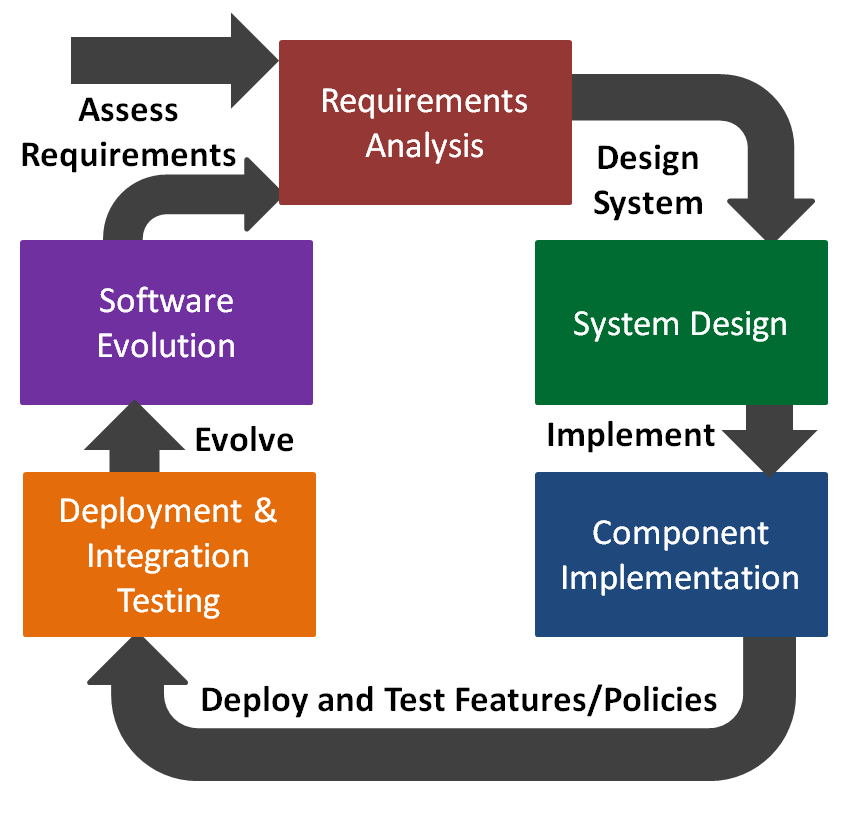
\includegraphics[width=0.9\linewidth]{sdlc}
		\caption{Industrial SDLC}
		\label{fig:sdlc}
	\end{subfigure}%
	\begin{subfigure}{.5\textwidth}
		\centering
		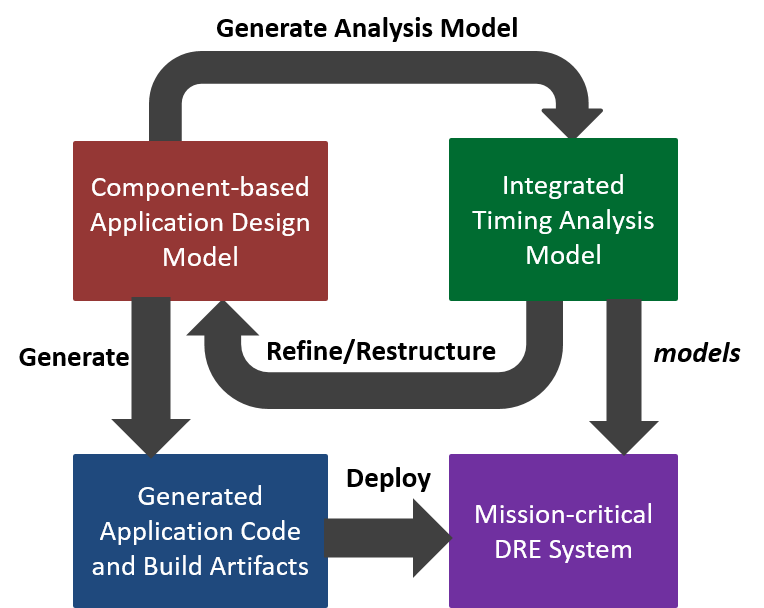
\includegraphics[width=\linewidth]{big_picture_2}
		\caption{DREMS Analysis-driven Workflow}
		\label{fig:big_picture}
	\end{subfigure}
	\caption{Embedded Software Development Lifecycle Comparison}
	\label{fig:test}
\end{figure}

Figure \ref{fig:sdlc} shows a \emph{spiral model} \cite{boehm1988spiral} of a typical industrial software/system development life cycle (SDLC). The five stages in this cycle include requirements analysis, software design, implementation, integration testing, and design evolution. Although the intricacies of each stage is hidden, the large majority of industrial software development follows this lifecycle. Embedded software development, especially for safety critical systems, does not lend itself well to this life cycle, mainly because the deliverable in such projects is usually not just a software package or a hardware platform but an amalgamation of both. Software development in fields like robotics, is tightly coupled with the hardware; assessment of software performance is sometimes dependent on and blocked by the hardware availability. Such blocking delays lead to inefficiencies in software evaluation and longer development times. It is also possible that design oversights could lead to poor timing performance e.g. long response times to critical events, that could damage the hardware in the process. Thus, the analysis presented in this work, supports and argues for a verification-driven workflow, as shown in Figure \ref{fig:big_picture}. The software evaluation is performed at design-time and as often as possible until the assembly is refined and optimized. Application developers use domain-specific modeling languages to structure large-scale component assemblies and modular code generation features to speed up software development efforts. Moreover, domain-specific properties such as interaction patterns, component execution code, and associated temporal properties such as worst-case execution times, deadlines etc. can be easily injected into such models. Using such application parameters in the \textit{design} model, a Colored Petri net-based (CPN) \cite{CPN} \textit{formal analysis model} is generated. The system behavior is both simulated and analyzed using a CPN execution engine, CPN Tools \cite{CPNTools}, and useful properties of the system are verified. By generating a bounded \emph{state space} of the system, the execution traces exhibited by the system are searched for property violations. Such system properties include the lack of deadlocks, deadline violations and worst-case trigger-to-response times. The goal of this analysis is to ensure that a component-based system: an assembly of tested component building blocks, meets the temporal specifications and requirements of the system.  

The results of this analysis will help improve the structure of the application, enabling safe deployment of dependable components that are known to operate within system specifications. Using CBSE also enables this restructuring process as the components are not tightly coupled software entities. So, when designing the integrated system, the analysis can be performed by assigning \emph{time budgets} to the discrete tasks in the execution. This enables timing analysis before implementation and also uses the time budgets as requirements for efficient code implementation. These budgets are often derived from some high-level requirements and appropriately distributed between the different components in the system. The analyzed system may not necessarily be complete, but instead be in a process of evolution. As the design progresses, the system requirements become concrete and the design is re-verified at each stage to ensure the consistency of all timing guarantees. 

The remainder of this dissertation is organized as follows. Chapter \ref{chapter:fundamentals} describes some fundamental concepts about distributed real-time systems, component-based software and some challenges in timing analysis. Chapter \ref{chapter:related-research} briefly describes general software testing and analysis methodologies, and summarizing related research in timing analysis and verification for distributed real-time embedded applications. Chapter \ref{chapter:DREMS} introduces the DREMS infrastructure and the Component Model used to experiment with and validate the timing analysis results. Chapter \ref{chapter:modeling} discusses the Colored Petri net-based timing analysis model devised for component-based DRE systems. Chapter \ref{chapter:analysis} describes the scope and efficiency of the analysis methods implemented with this CPN model. Chapter \ref{chapter:evaluation} evaluates this model with published results on analysis design, scalability and experimental validation. Finally, Chapter \ref{chapter:conclusion} concludes the dissertation, providing a summary of the detailed work and describing potential future work.
\chapter{Fundamentals}
\label{chapter:fundamentals}

A real-time system \cite{liu2000real} is one where the correctness of the system behavior is dependent not only on the logical results of the computation but also on the physical time when these results are produced. Here, the system \emph{behavior} refers to the sequence of outputs over time of the system. The flow of time is modeled as a directed line that extends from the past into the future. A slice of time in this line is called an \emph{instant}. Any ideal (expected) occurrence at a time instant is called an \emph{event}. An interval on this time line is called the \emph{duration}, defined by two events, the start event and the end or terminating event. This timeline is discrete when the time line is partitioned into a sequence of equally spaced durations, called clock \emph{ticks}. A real-time system typically changes as a function of physical time i.e. a non-spatial continuum in which events occur in apparently irreversible succession from the past through the present to the future. If the real-time system is \emph{distributed}, then it consists of a set of computers, \emph{nodes}, interconnected by a real-time communication network.

% Describe Real-time Systems
Real-time systems are subject to strict operational deadlines. These deadlines constrain the amount of time permitted to elapse between a stimulus provided to the system and a response generated by the system. Consequently, the correctness of such systems depends heavily on its temporal and functional behavior. Real-time programs that are logically correct i.e. implement the intended functions, may not operate correctly if the required timing properties are not met. Typically, such systems are classified as either soft or hard real-time systems. In soft real-time systems, missing deadlines does not completely degrade the overall system performance e.g. delays in opening a web browser does not render the web browser useless; the browser, as an entity is still functional. Hard real-time systems, however, are systems where missed deadlines could be critical e.g. delays in pacemaker timing cycles leads to irregular heart beats with potentially fatal consequences. It is important that any error within the system e.g. data loss or corruption, node failure etc. be detected within a short time with a very high probability. The required error-detection latency must often be in the same order of magnitude as the sampling period of the fastest critical control loop. Then, it is possible to perform corrective action, or bring the system to a safe state. This makes the design of hard real-time systems different from soft real-time systems. The demanding response time requirements, often in milliseconds or less, preclude human intervention during normal operation. A hard real-time system must be highly autonomous to maintain safe operation. In contrast, the response time requirements of soft real-time systems is often in the order of seconds. 

% Components in a real-time system model
%A Cyber-Physical System (CPS) can be decomposed into three communicating entities; (1) a controlled object; could be a physical subsystem, (2) a (potentially distributed) computer system executing programs, and (3) a human user. The computer system consists of computational nodes that interact by exchanging messages. Each node can host one or more computational \emph{components}. In this model, a component is a self-contained hardware/software unit that interacts with its environment by exchanging messages. A timed sequence of output messages that a component produces represents its \emph{behavior}. An unintended \emph{faulty} behavior can lead to a \emph{failure}. A real-time component contains a real-time clock i.e. a high-precision clock that keeps track of the current time, and is thus aware of the progression of time. Real-time clocks are used in a variety of modern embedded systems e.g. digital cameras where a \emph{timestamp} is needed. 

%When triggered, a component starts executing its predefined computations at the start instant. The communication infrastructure provides for the transport of \emph{messages} from a sender component to one or more receiver components within a given interval of time. A message is sent at a \emph{send instant} and received at the receiver at some later \emph{receive instant}. The temporal properties of a messaging system include information about the temporal order, the send instant and latency of transport. A message contains a data field that holds a data structure that is transported between components. The communication interface is agnostic about the contents of this data field. 

%The \emph{state} of a real-time component represents a separation between past and future component behaviors i.e. there must be a consistent temporal order among the events of significance to a component. Component states enable the determination of a future output solely on the basis of the future input and the present state of the system i.e. state embodies all of system history. Here, a component is a self-contained validated unit that can be used as a building block in the construction of larger systems. In order to enable a composition of a component into a distributed set of components, the principle of \emph{composability} should be observed. A set of components are said to be composable with respect to a specified property if the system integration will not invalidate this property, once the property has been established on the subsystem level. Examples of such properties include timeliness or testability. In composable systems, the system properties follow from the properties of the individual components. This means that in a composed architecture, the introduced abstraction of a component must remain intact, even if the component becomes faulty i.e. it must be possible to replace a faulty component without any knowledge about the component internals. Note that this principle constrains the implementation of a component, because it restricts the implicit sharing of resources among components; if a shared resource fails, more than one component is affected by the failure. 

Timing and schedulability analysis in real-time systems usually assumes an ideally functioning software program where every step of computation performs as expected and characterizes these steps with timing properties such as worst-case execution times (WCET) \cite{wilhelm2008worst} or response times \cite{joseph1986finding}. Once a \emph{timing model} of the system is realized, the behavior can be analyzed by using either a discrete event simulator, prototypical testing or formal analysis methods. This thesis concentrates on a formal analysis approach to analyzing the temporal behavior of a class of distributed real-time embedded systems.

\emph{Verification} establishes a consistency between the formal system specification and the system requirements, and also between the specification and the implementation, while \emph{validation} is concerned with the consistency between the model of the user's intentions and the system requirements. The missing link between verification and validation is the relationship between the user's expectations and the final system as built i.e. validation can be done on multiple artifacts but ultimately the system should meet the client's expectations. Discrepancies between these notations are called \emph{system specification errors}. Verification is usually reduced to a mathematical analysis process, while validation must examine the system's behavior in the real-world. If properties of a system have been formally verified, it still has not been established whether the existing formal specification captures all the aspects of the intended behavior in the user's real-world environment. To be free of specification errors, validation and specification testing are required for quality assurance. The primary verification method is \emph{formal analysis} and the primary validation method is \emph{testing}. The following chapter reviews various general analysis methodologies, including system-level or acceptance testing and formal verifications methods, and also selective system-level analysis methodologies for concurrent real-time systems that are related to this dissertation. 

\if 0

There are several challenges to modeling and analysis of such distributed safety-critical systems. Using real-time components that can run on heterogeneous hardware platforms means that the components have different timing characteristics on the different platforms. Therefore, a component must be molded and re-verified for each hardware platform on which it is deployed. Secondly, component-based systems are constructed by assembling a tested set of components. Two components that individually provide timing guarantees may not aid the overall system-level requirements when executed concurrently in a specific hardware platform. The challenge here is ensuring that a system consisting of composed set of verified components still retains its timing behavior. Thus, the requirements for timing analysis become two fold: 

\begin{itemize}
	\item Verify the timing properties of each component in the system - Does the operational behavior of a software component meet its timing requirements?
	
	\item Analyze the schedulability of a component assembly - When composed together, do all components work as expected to meet the end-to-end system-wide timing requirements?
\end{itemize}

The results of this two-level timing analysis should indicate with sufficient proof the stability or instability of the composed component-based system. Achieving this workflow is the fundamental goal of our timing analysis methodology, presented in later sections. Our analysis model uses a Colored Petri Net \cite{CPN} based formal analysis methodology. However, motivating this methodology requires first an in-depth literature review. The following section reviews both general analysis methodologies used in the past, and specific system-level modeling and timing analysis techniques for concurrent real-time systems, along with advantages, limitations and potential improvements that motivate our presented work.

\fi
\section{Related Research}
\label{sec:Related_Research}

% MAST
Verification of component-based systems requires significant amount of information about the application assembly, interaction semantics, and real-time properties. This information is primarily derived from the design model although many real-time metrics are not explicitly modeled. Using model descriptors, \cite{Lopez2006} describes interaction semantics and real-time properties of components. Using the MAST modeling and analysis framework \cite{MAST1, MAST2}, schedulability analysis and priority assignment automation is supported. Event-driven models are separated into several \emph{views} which are similar to hierarchical pages in some modeling formalisms, like Colored Petri Nets (CPN). Analysis efforts include the calculation of response times, blocking times, and slack times. %For every real-time application, a separate and independent real-time analysis model is generated for each mode of operation and analyzed

High-level Petri nets are a powerful modeling formalism for concurrent systems and have been integrated into many modeling tool suites for design-time verification. General-purpose Architecture Analysis \& Design Language (AADL) models have been translated into symmetric nets for qualitative analysis \cite{kordon_sn} and Timed Petri nets \cite{kordon2009} to check real-time properties such as deadline misses, buffer overflows etc. Similar to \cite{kordon2009}, our CPN-based analysis also uses bounded observer places \cite{Alpern1989} that observe the system behavior for property violations and prompt completion of operations. However, \cite{kordon2009} only considers periodic threads in systems that are not preemptive. Our analysis is aimed at a combination of preemptive and non-preemptive hierarchical scheduling with higher-level component interaction concepts. separately.

Several analysis approaches present tool-aided methodologies that exploit the capabilities of existing analysis and verification techniques. In the verification of timing requirements for composed systems, \cite{medina2011} uses the OMG UML Profile for Modeling and Analysis of Real-Time and Embedded Systems (MARTE) modeling standard and converts high-level design into MAST output models for concrete schedulability analysis. In a similar effort, AADL models are translated into real-time process algebra \cite{sokolsky2006} reducing schedulability analysis into a deadlock detection problem searching through state spaces and providing failure scenarios as counterexamples. Symbolic schedulability analysis has been performed by translating the task sets into a network timed automata, describing task arrival patterns and various scheduling policies. TIMES \cite{TIMES} calculates worst-case response times and scheduling policies by verifying timed automata with UPPAAL \cite{UPPAAL} model checking.

In order to analyze hierarchical component-based systems, the real-time resource requirements of higher-level components need to be abstracted into a form that enables scalable schedulability analysis. The authors in \cite{easwaran2006} present an algorithm where component interfaces abstract the minimum resource requirements of the underlying components, in the form of periodic resource models. Using a single composed interface for the entire system, the component at the higher level selects a value for operational period that minimizes the resource demands of the system. Such refinement is geared towards minimum waste of system resources.

\chapter{Design Model: Distributed Managed Systems (DREMS)}
\label{chapter:DREMS}

\section{DREMS Component Model}

Timing analysis of component-based software, as presented in this dissertation, is facilitated by the DREMS component model (\iapfull) \cite{DREMS13Software} \cite{ISIS_F6_ISORC:13}. DREMS was designed and implemented for the class of distributed real-time embedded systems that are remotely deployed and characterized by strict timing requirements e.g. a cluster of satellites, UAV swarms, disaster relief robots etc. DREMS is a software infrastructure for the design, implementation, deployment and management of component-based distributed real-time embedded systems. The infrastructure includes design-time modeling tools \cite{ISIS_F6_SFFMT:13} that integrate with a well-defined and fully implemented component model \cite{ISIS_F6_ISORC:13, kumar2014colored} used to build component-based applications. Rapid prototyping and code generation features coupled with a modular runtime platform automate the tedious aspects of the software development and enable robust deployment and operation of mixed-criticality distributed applications. This chapter elaborates on the DREMS component model, the operation execution semantics, and the process scheduling aspects i.e. properties of the DREMS software stack that are relevant for generating a timing analysis model.

%The DREMS component model is based on the Component Integrated ACE ORB (CIAO) \cite{RT_CIAO:04, CIAO_Chap:04} project. CIAO is an implementation of the OMG's Lightweight CORBA Component Model (CCM) \cite{CCM-light:03}. CIAO uses the TAO~\cite{TAO:02} CORBA object request broker (ORB) as its default underlying communication middleware.  With the recent standardization of connector mechanisms~\cite{dds4ccm:09}, CIAO is also able to support asynchronous messaging and the OMG Data Distribution Service (DDS) through its ports. Unlike CIAO, the DREMS component model is not tightly coupled with the CORBA transport mechanisms. All component communication is via ports and connectors \cite{Connectors} enabling a variety of interaction schemes. 

\begin{figure}[h]
	\centering
	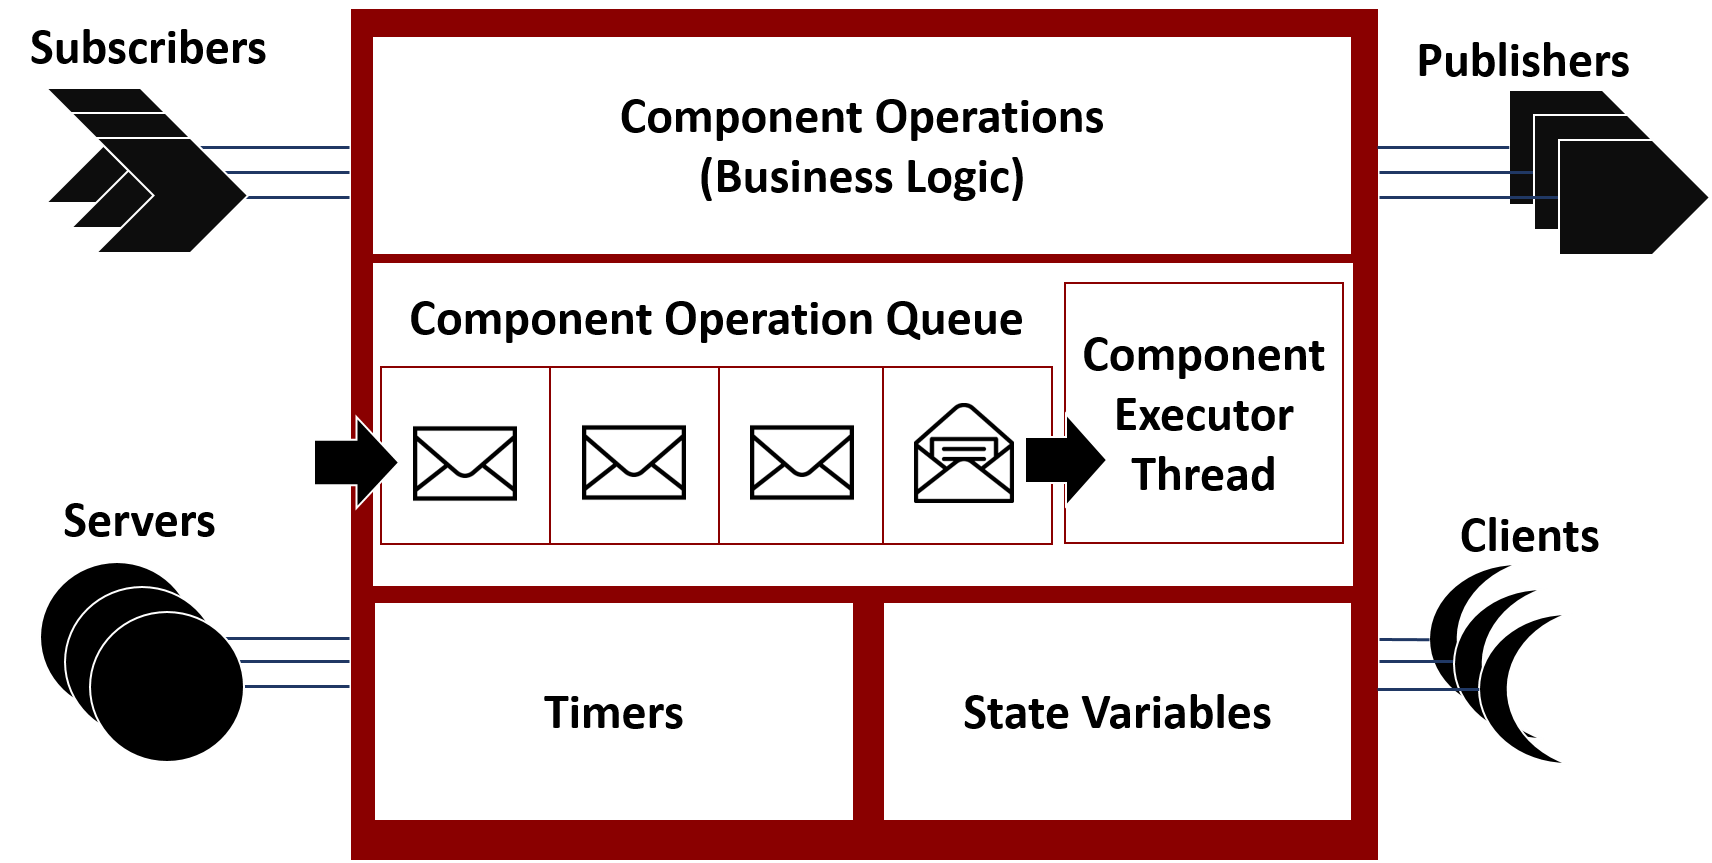
\includegraphics[width=\textwidth]{ROSMOD_Component}
	\caption{DREMS Component}
	\label{fig:DREMS_Component}
\end{figure}


Figure \ref{fig:DREMS_Component} presents a typical DREMS-style component. Component-based software engineering relies on the principle of assembly -- large and complicated systems can be iteratively constructed by composing small reusable component building blocks. Each \emph{component} contains a set of communication ports and interfaces, a message queue, time-triggered event handling and state variables. Using ports, components communicate with the external world. Using interfaces and message passing schemes, components process requests from other components. This interaction mechanism lies at the heart of component-based software. Each DREMS component supports four basic types of ports for interaction with other collaborating components: Facets, Receptacles, Publishers and Subscribers. A component's {\bf facet} is a unique interface that it exposes to its clients. This interface can be invoked either synchronously via remote method invocation (RMI) or asynchronously via asynchronous method invocation (AMI) \cite{waldo1998remote, raje1997asynchronous}. A component's {\bf receptacle} specifies an interface required by the component in order to function correctly. Using its receptacle, a component can invoke operations on other components using either RMI or AMI. A {\bf publisher} port is a single point of data emission. This port emits data produced by a component operation. A {\bf subscriber} port is a single point of data consumption, feeding received data to the associated component. Communication between publishers and subscribers is contingent on the compatibility of their associated topics. Publishers and Subscribers enable the OMG DDS anonymous publish/subscribe \cite{eugster2003many} style of messaging. More details on this component model can be found in ~\cite{ISIS_F6_ISORC:13}.

\section{Component Execution Semantics}

An \emph{operation} is an abstraction for the different tasks undertaken by a component. These tasks are implemented by the component's source code written by the developer. Application developers provide the functional, \emph{business-logic} code that implements operations on local state variables and inputs received on component ports. For example, a proportional integral differential control operation could receive the current state of dynamic variables from a \emph{sensor} component, and using the relevant gains, calculate a new state to which an \emph{actuator} component should progress the system. In order to service interactions with the underlying framework and with other components, each component has a \emph{message queue}. This queue holds operation requests received from the external environment i.e. messages, service requests or responses, and timer activations. Each request is characterized by a priority and a deadline. Priority refers to the relative importance of one operation over another within the scope of the component. Deadline refers to the worst-case duration of time that an operation can take to complete. If the execution of the operation takes beyond its deadline to complete, then a \emph{deadline violation} is said to have occurred.   

DREMS component execution is handled by a single executor thread. This executor thread picks the next available request from the message queue and executes the operation to completion i.e. the operation scheduling is non-preemptive. So, all operations in the queue, regardless of priority, need to wait for the currently executing operation to complete. Allowing only a single executor thread per component and enforcing a single-threaded non-preemptive scheduling scheme on the operations helps avoid synchronization primitives for internal state variables and establishes a more easily analyzable system. It is true that multi-threaded solutions to operation scheduling would avoid starvation i.e. operations in the queue will not have to wait forever if the currently executing operation is blocked on a resource. We address such cases in our experimental evaluation (Section \ref{sec:long_running_operations}). However, the DREMS execution semantics is still the more predictable design as it is more easily analyzable. The non-determinism in multi-threaded executions causes a tree of possible behaviors, leading to a common analysis challenge called state space explosion \cite{lin1987protocol}. Keeping the operation execution to a single thread per component bounds the overall number of threads in the system leading to a more tractable analysis. 

\begin{figure}[ht]
	\centering
	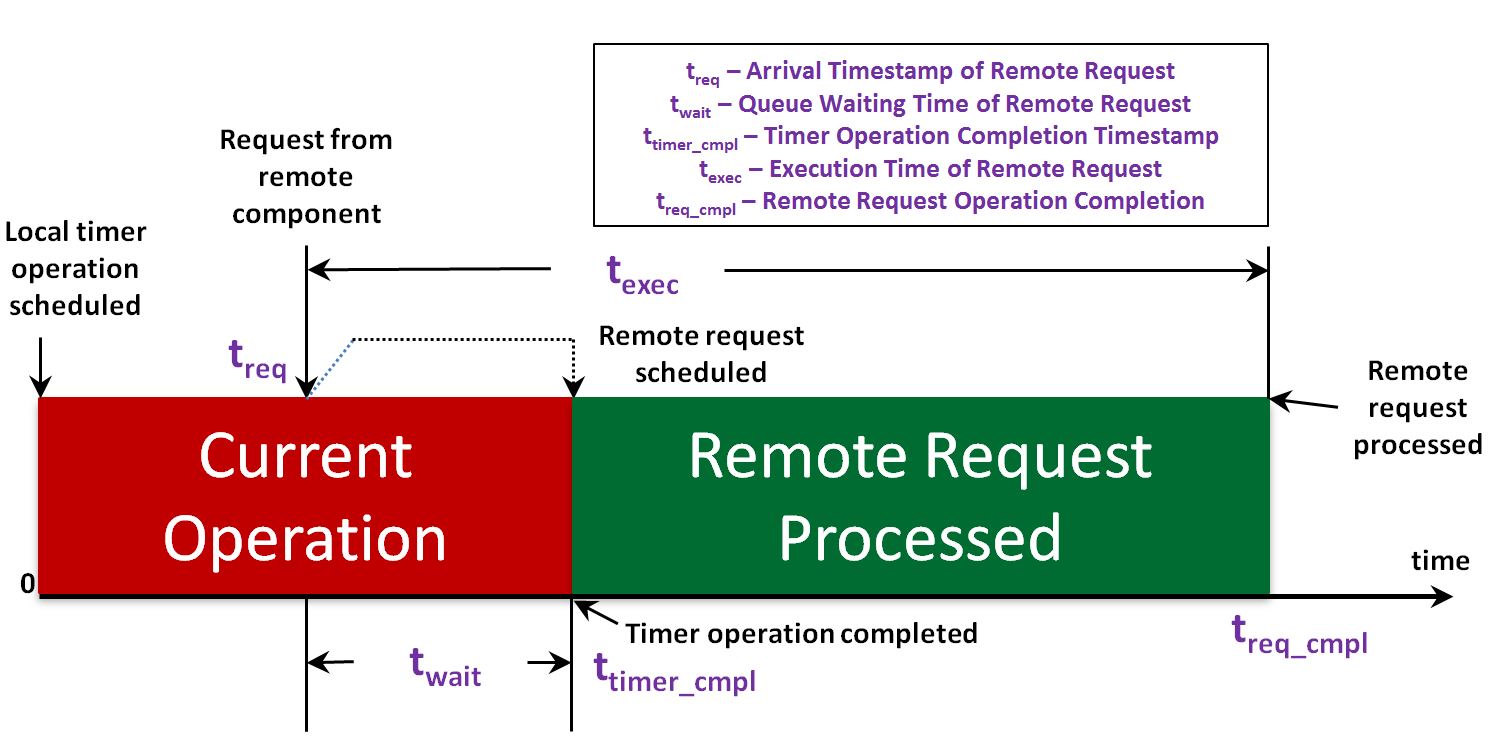
\includegraphics[width=\textwidth]{cop_execution_semantics}
	\caption{Component Operation Execution Semantics: This figure shows the effects of the ROSMOD component scheduling on an incoming operation request. $t\_{req}$ represents the arrival time of a remote request. $t\_{wait}$ is the wait time of this request in the message queue while the current operation is still executing. $t\_{timer\_cmpl}$ is the time stamp at which the current operation completes executing. At this time, the remote request is finally scheduled for execution. $t\_{req\_cmpl}$ is the time stamp at which the remote request completes. The execution time, $t\_{exec}$ of this request is calculated as the difference in time stamps between $t\_{req\_cmpl}$ and $t\_{req}$.}
	\label{fig:cop_execution_semantics}
\end{figure}

Figure \ref{fig:cop_execution_semantics} shows the execution semantics of a component operation executed on the component's executor thread. Simplifying assumptions include that this component is the only component thread executing on the CPU and the CPU is a single core one. Assume that at $t=0$, this component is processing the expiry of a local timer. This operation is expected to complete at $t = t_{timer\_cmpl}$. However, at $t = t_{req}$, a service request is received from some remote component. Since the component operation scheduling is non-preemptive, regardless of the priority of this service, the request is not processed until $t_{timer\_cmpl}$. Therefore, the request is waiting in the message queue for $t_{wait} = t_{timer\_cmpl} - t_{req}$. At $t = t_{timer\_cmpl}$, the timer operation is marked as complete and the service request is processed. The total execution time of this service operation (also called its response time) is calculated by including the duration of the time for which this request waited in the component message queue i.e. $t_{exec} = t_{req\_cmpl} - t_{req}$. 

This is a simple scenario showing how a single operation on a single component is affected by the operation scheduling semantics. The wait times of the remote request are also worsened by OS scheduling non-determinism -- when multiple components are scheduled concurrently, fixed-priority real-time scheduling is enforced. If the executor threads of various components are of different priorities, then the highest priority ready executor thread is always chosen. If these threads are of equal priority, then round-robin scheduling is carried out. Round-robin scheduling assigns a fixed time slice to each thread in equal portions and in circular order, handling all threads without priority. %The analysis of equal priority threads is performed by making no assumptions about the initial order i.e. any one of the equal priority threads is chosen at random and then a random circular order is established for round-robin scheduling. This causes non-determinism in the thread picking order and therefore also in the wait times of the operations executed by each thread. 

\section{Temporal Partition Scheduler}

DREMS components are grouped into processes that are assigned to temporal partitions, implemented by the DREMS OS scheduler. This scheduler was implemented by modifying the behavior of the standard Linux scheduler, introducing an ARINC-653 ~\cite{ARINC-653} style temporal and spatial partitioning scheme. 

\begin{figure}[ht]
	\centering
	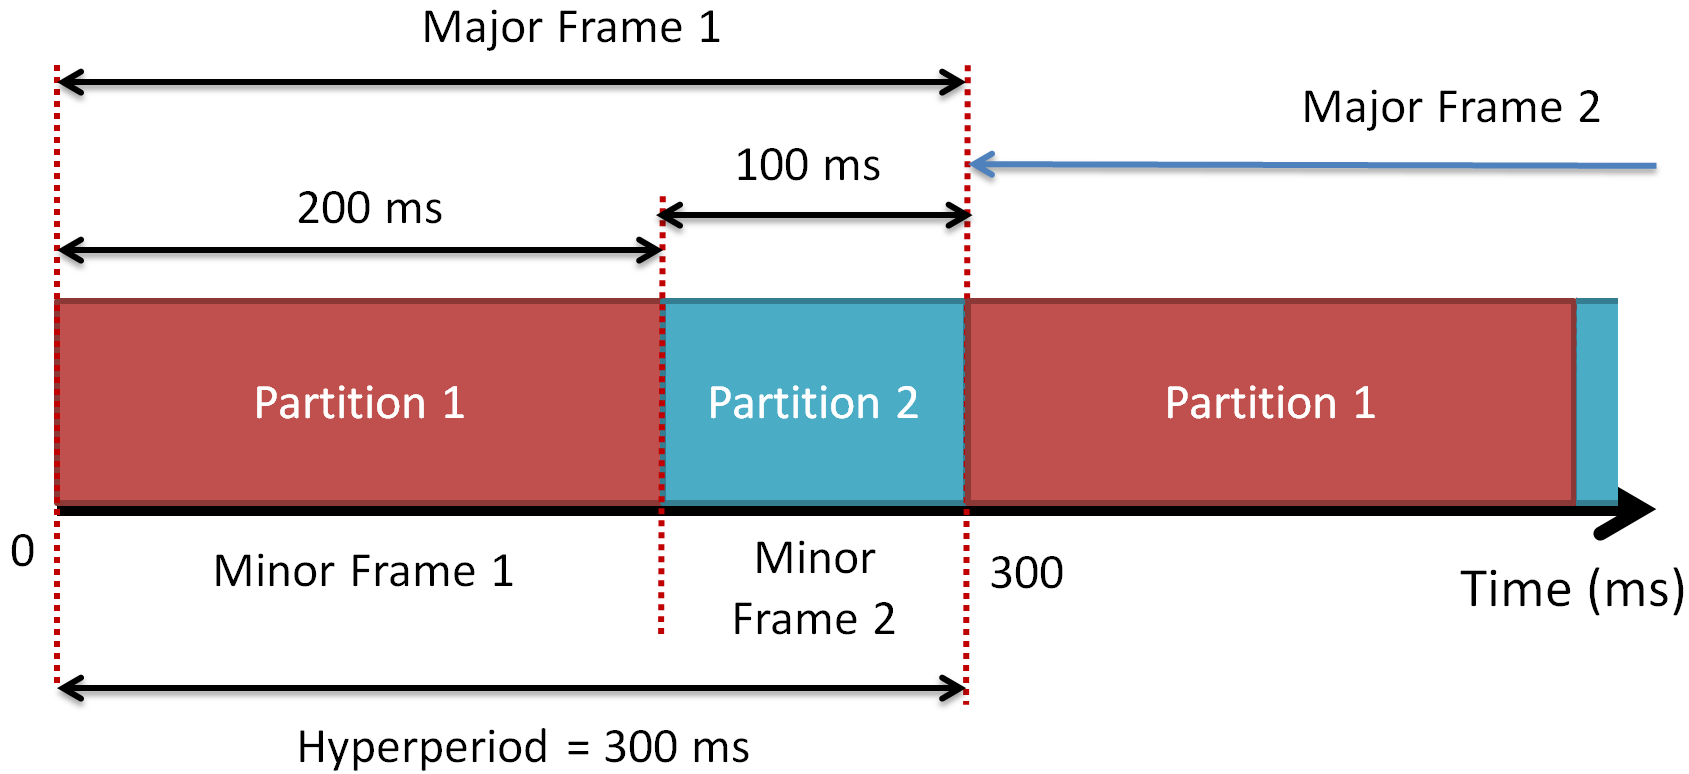
\includegraphics[width=\textwidth]{partition_scheduling}
	\caption{Sample Temporal Partition Schedule with Hyperperiod = 300 ms}
	\label{fig:partition_scheduling}
\end{figure}


Temporal partitions are periodic fixed intervals of the CPU's time. Threads associated with a partition are scheduled only when the partition is active. This enforces a temporal isolation between processes assigned to different partitions. The repeating partition windows are called \emph{minor frames}. The aggregate of repeating minor frames is called a \emph{major frame}. The duration of a major frame is called the \emph{hyperperiod}, which is typically the lowest common multiple of the partition periods. Each minor frame is characterized by a period and a duration. The period specifies how often this partition becomes active and the duration defines how much of the CPU time is available for scheduling the runnable threads associated with that partition. Figure \ref{fig:partition_scheduling} shows a sample temporal partition schedule. 

The DREMS component model supports non-functional properties e.g. timeliness, fault tolerance and security as an integral part of the design. Every operation on a component is associated with a deadline. Timed triggers can be associated with operations/callbacks that dictate when and how frequently certain operations are scheduled. Deadline monitoring is invoked when an operation is allowed to execute i.e. enqueued on the component message queue. The component thread that releases the business logic execution thread monitors the deadline. If a hard deadline is reached but the operation is incomplete, then the infrastructure notifies a local fault manager and appropriate actions are taken. 

Also, some long-term mission profiles e.g. space missions may involve long running computations and sensor-driven periodic calculations. Since the component execution semantics allows only one active operation to execute at a time within a component, it is possible that a ready operation is blocked for prolonged periods of time by an operation waiting on some I/O device. In such scenarios, developers can opt into using blocking I/O operations, polling mechanisms and asynchronous nonblocking I/O operations. In a blocking I/O task, the component is unavailable while the operation is running. Other components may execute in the system, but the one waiting on an I/O device is blocked. This blocking could propagate to other components and introduce significant delays. When using polling, some periodic task is scheduled that checks for the completion of I/O interaction. This leads to a potential waste of resources and decreased performance. Lastly, the component model supports asynchronous I/O, where the component triggers an I/O interaction and returns to handle other operations in the queue. The component does not block on the I/O and is notified when the I/O task completes. Such varied interaction patterns makes this component model very generic and a suitable target for our timing analysis work. The rich interactions and communication mechanisms are inspired by other common industrial component models such as CIAO \cite{CIAO_Chap:04} and ACM \cite{ACM_SPE:10}, and the execution semantics are precisely defined and implemented. A qualitative evaluation of its capabilities \cite{ISIS_F6_ISORC:13} show that although the model was designed for fractionated spacecraft, DREMS is suitable for a variety of distributed and embedded environments. 
\section{Colored Petri Net-based Analysis Model}
\label{sec:Colored_Petri Net-based_Analysis_Model}

This section briefly describes how Colored Petri nets (CPN) are used to build an extensible, scalable analysis model for component-based applications. Several nets are used to compose the different layers of the design model. To edit, simulate and analyze this model, we use the CPN Tools \cite{CPNTools} tool suite. The tool suite includes a simulator, as well as a state-space analysis tool that computes the (bounded) state space of the system under execution. The analysis model is based on the formal component model, i.e. the model of computation used. For a different component execution semantics, this model needs to be adjusted. 

\subsection{Model of Time}
Appropriate choice for temporal resolution is a necessary first step in order to model and analyze threads running on a processor. The OS scheduler enforces temporal partitioning and uses a priority-based scheme for threads active within a temporal partition. If multiple threads have the same priority, a round-robin (RR) scheduling is used. In order to observe and analyze this behavior, we have chosen the temporal resolution to be 1 ms; a fraction of 1 clock tick of the OS scheduling quantum. 
\subsubsection{Dynamic Time Progression}
Although the time resolution at the start of the analysis is chosen to be 1 ms, this is not a constant throughout the execution of the analysis model. If it were then \emph{S} seconds of activity will generate a state space of size: $SS_{size} = \sum\limits_{i=1}^{S*1000} TF_{t_i}$
%\vspace{-0.2in}
%
%\begin{equation}
%\begin{split}
%SS_{size} = \sum\limits_{i=1}^{S*1000} & TF_{t_i}
%\end{split}
%\end{equation}
where $TF_{t_i}$ is the number of state-changing CPN transition firings between $t_i$ and $t_{i+1}$. This large state space includes intervals of time where there is no thread activity to analyze either due to lack of operation requests, lack of ready threads for scheduling, or due to temporal partitioning. During such idle periods, the analysis engine dynamically increases the time-step size and progresses time either to (1) the next node-specific clock tick, (2) the next global timer expiry offset, or (3) the next node-specific temporal partition (whichever is earliest and most relevant). This ensures that the generated state space tree is devoid of nodes where there is no thread activity. Such dynamic control of time using global variables during analysis is also one of the advantages of using colored Petri nets. 

\subsection{Modeling Component-based Applications}

\begin{figure}[htb]
	\centering
	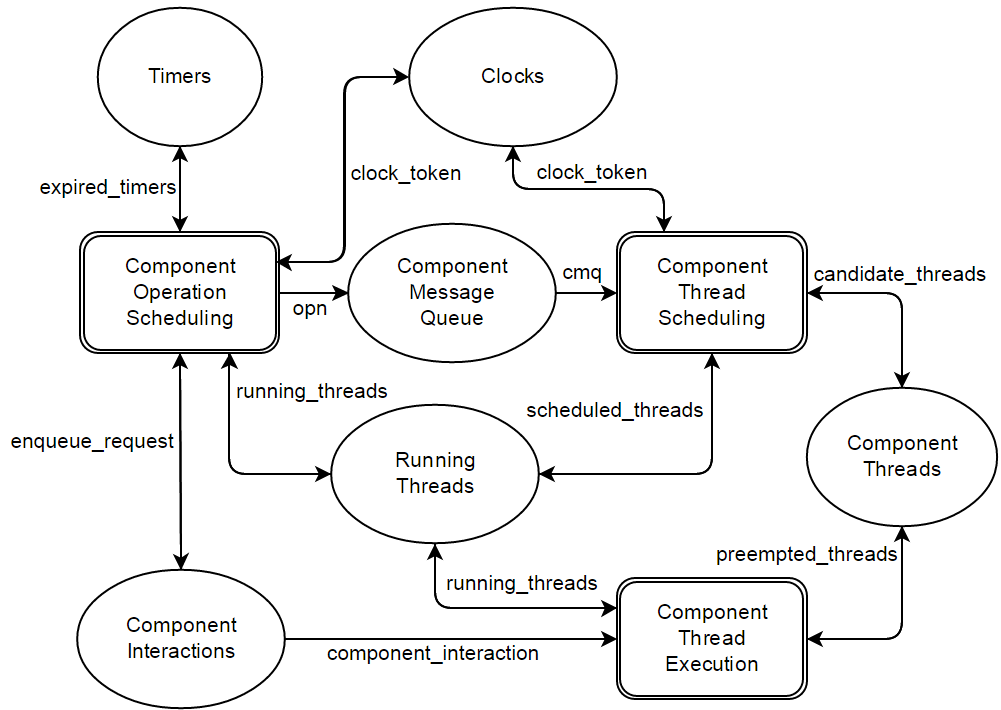
\includegraphics[width=0.45\textwidth]{figs/HL_CPN.png}
	\caption{Top-level CPN Model}
	\label{fig:hl_cpn}
\end{figure}

The top-level CPN Model is shown in Figure \ref{fig:hl_cpn}. The places (shown as ovals) in this model maintain \emph{colored} (typed) tokens that represent the states of interest for analysis. For instance, the \emph{Clocks} place holds tokens of type \emph{clock\_tokens} maintaining information regarding the state of the clock values and temporal partition schedule on all computing nodes. To ensure modularity, this model is partitioned into two interacting sub-nets to handle the hierarchical scheduling.

\subsubsection{Component-level Execution Model}

\paragraph{Component Operations} Every operation request \emph{O} made on a component \emph{$C_x$} is a \emph{record} type implementation of the 4-tuple:

\vspace{-0.15in}
\begin{equation}
O(C_x) = \ < ID_O, \ Prio_O, \ Dl_O, \  Steps_O >
\end{equation}

where, $ID_O$ is a unique concatenation of strings that help identify and locate this operation in the system (consisting of the name of the operation, the component, the computing node, and the temporal partition). The operation's priority ($Prio_O$) is used by the analysis engine to enqueue this operation request on the message queue of $C_x$ using a fixed-priority non-preemptive FIFO scheduling scheme. The completion of this enqueue implies that this operation has essentially been \emph{scheduled} for execution. Once enqueued, if this operation does not execute and complete before its fixed deadline ($Dl_O$), its real-time requirements are violated. 

\paragraph{Steps} 
\label{para:steps}

Once an operation request is dequeued, the execution of the operation is modeled as a transition system that runs through a sequence of steps dictating its behavior. Any of these underlying steps can have a state-changing effect on the thread executing this operation. For example, interactions with I/O devices on the component-level could block the executing thread (for a non-deterministic amount of time) on the OS-level. Therefore, every component operation has a unique list of steps ($Steps_O$) that represent the sequence of local or remote interactions undertaken by the operation. Each of the \emph{m} steps in $Steps_O$ is a 4-tuple:

\vspace{-0.15in}
\begin{equation}
s_i = \ <Port, \ Unblk_{s_i}, \ Dur_t, \ Exec_t>
\end{equation}

where $1 \le i \le m$. \emph{Port} is a \emph{record} representing the exact communication port used by the operation during $s_i$. $Unblk_{s_i}$ is a list of component threads that are unblocked when $s_i$ completes. This list is used, e.g., when the completion of a synchronous remote method invocation on the server side is expected to unblock the client thread that made the invocation. Finally, temporal behavior of $s_i$ is captured using the last two integer fields: \emph{$Dur_t$} is the worst-case estimate of the time taken for $s_i$ to complete and $Exec_t$ is the relative time of the execution of $s_i$, with $0 \le Exec_t \le Dur_t$.

\paragraph{Component Interactions}

Consider an application with two components: a client and a server. The client is periodically triggered by a timer to make an remote method call to the server. We know that when the client executes an instance of the timer-triggered operation, a related operation request is enqueued on the server's message queue. In reality, this is handled by the underlying middleware. Since we do not model the details of this framework, the server-side request is modeled as an \emph{induced operation} that manifests as a consequence of the client-side activity. Tokens that represent such design-specific interactions are maintained in the place \emph{Component Interactions} (Figure \ref{fig:hl_cpn}) and modeled as shown in equation \ref{eq:component_interactions}. The interaction \emph{Int} observed when a component $C_x$ queries another component $C_y$ is modeled as the 3-tuple:

\vspace{-0.15in}
\begin{equation}
\label{eq:component_interactions}
Int(C_x, C_y) = \ < Node_{C_x}, \ Port_{C_x}, \ O(C_y)>
\end{equation}

When an operational \emph{step} in component $C_x$ uses port $Port_{C_x}$ to invoke an operation on component $C_y$, the request $O_{C_y}$ is enqueued on the message queue of $C_y$. %As shown in Figure \ref{fig:hl_cpn}, the transition \emph{Component Operation Scheduling} observes the \emph{Running Threads} at every time step to check for completion of external interaction requests. When satisfied, the necessary operation token is removed from \emph{Component Interactions} and enqueued onto the appropriate message queue.

\paragraph{Timers}

DREMS components are inactive initially; once deployed, a component executor thread is not eligible to run until there is a related operation request in the component's message queue. To start a sequence of component interactions, periodic or sporadic timers can be used to trigger a component operation. In CPN, each timer $TMR$ is held in the place \emph{Timers} and represented as shown in Eq. \ref{eq:TMR}. Timers are characterized by a period ($Prd_{TMR}$) and an offset ($Off_{TMR}$). Every timers triggers a component using the operation request $O_{TMR}$.

\vspace{-0.15in}
\begin{equation}
\label{eq:TMR}
TMR = \ < Prd_{TMR}, \ Off_{TMR}, \ O_{TMR}>
\end{equation}

\subsubsection{OS-level Execution Model}

\paragraph{Temporal Partitioning}
The place \emph{Clocks} in Figure \ref{fig:hl_cpn} holds the state of the node-specific global clocks. The temporal partition schedule modeled by these clocks enforces a constraint: component operations can be scheduled and component threads can be run only when their parent partition is active. Each clock token \emph{NC} is modeled as a 3-tuple:

\vspace{-0.15in}
\begin{equation}
\label{eq:NC}
NC = \ < Node_{NC}, \ Value_{NC}, \ TPS_{Node_{NC}} >
\end{equation}

where, $Node_{NC}$ is the name of the computing node, $Value_{NC}$ is an integer representing the value of the global clock and $TPS_{Node_{NC}}$ is the temporal partition schedule on $Node_{NC}$. Each \emph{TPS} is an ordered list of temporal partitions.

\vspace{-0.15in}
\begin{equation}
\label{eq:TP}
TP = \ < Name_{TP}, \ Prd_{TP}, \ Dur_{TP}, \ Off_{TP}, \ Exec_{TP} >
\end{equation}

Each partition $TP$ (Eq. \ref{eq:TP}) is modeled as a record color-set consisting of a name $Name_{TP}$, a period $Prd_{TP}$, a duration $Dur_{TP}$, an offset $Off_{TP}$ and the state variable  $Exec_{TP}$. %Aggregate of such partitions can fully describe a partition schedule. Complete partition schedules are maintained per computing node.

\paragraph{Component Thread Behavior}

Figure \ref{fig:Thread_Execution} presents a simplified version of the CPN to model the thread execution cycle. The place \emph{Component Threads} holds tokens that keep track of all the ready threads in each computing node. Each component thread $CT$ is a record characterized by:

\vspace{-0.15in}
\begin{equation}
\label{eq:CT}
CT = \ <ID_{CT}, \ Prio_{CT}, \ O_{CT}>
\end{equation}

where $ID_{CT}$ constitutes the concatenation of strings required to identify a component thread in CPN (i.e. component name, node name and partition). Every thread is characterized by a priority ($Prio_{CT}$) which is used by the OS scheduler to schedule the thread. 
%The DREMS OS uses a fixed-priority preemptive scheduling scheme (constrained by temporal partitioning) to schedule component threads. %If multiple threads belonging to the same temporal partition are ready, the highest priority thread is always chosen for execution. If there is more than one candidate thread, one is chosen at random, followed thereafter by a Round-Robin scheduling scheme. 

\vspace{-0.1in}
\begin{figure}[htb]
	\centering
	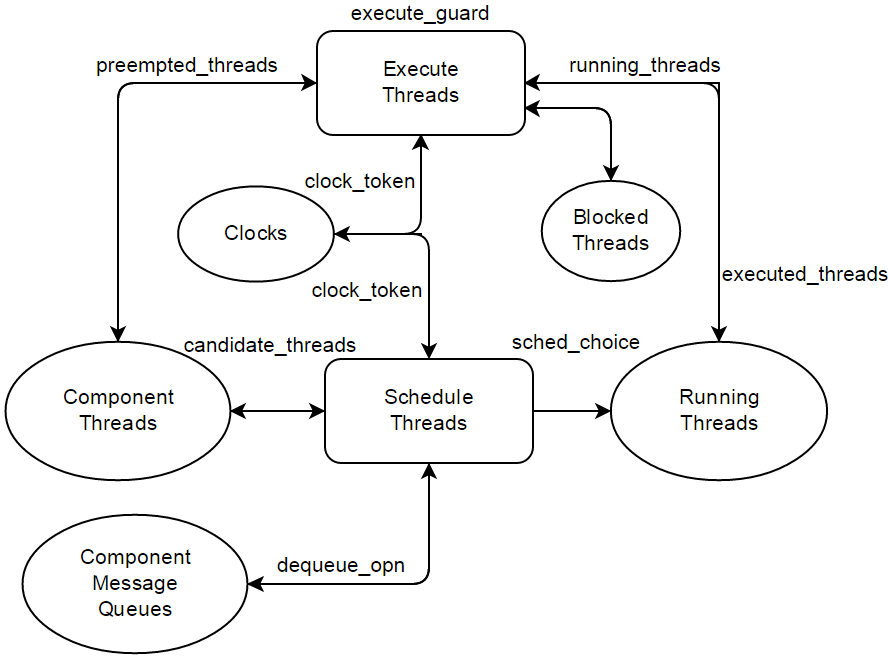
\includegraphics[width=0.40\textwidth]{figs/Thread_Execution.png}
	\caption{Component Thread Execution Cycle}
	\label{fig:Thread_Execution}
\end{figure}

If the highest priority thread is not already servicing an operation request, the highest priority operation from \emph{Component Message Queues} is dequeued and scheduled for execution (held by $O_{CT}$). The scheduled thread is placed in \emph{Running Threads}. %The guard on \emph{Schedule Thread} ensures that the highest priority thread in the currently running partition is scheduled first. 

When a thread token is marked as running, the model checks to see if the thread execution has any effect on itself or on other threads. These state changes are updated using the transition \emph{Execute Thread} which also handles time progression. Keeping track of $Value_{NC}$, the thread is preempted at each clock tick. This loop repeats forever, as long as there are no system-wide deadlocks. 

%It must be noted that system-critical processes such as deployment and fault management processes running periodically (or sporadically) at higher priorities than component processes are not necessarily affected by temporal partitioning. Such processes are scheduled to execute in a \emph{SYSTEM} partition when ever ready. Therefore when simulating the scheduling of such process threads, $TPS_{Node_{NC}}$ in equation \ref{eq:NC} is ignored.





\chapter{State Space Analysis and Verification}
\label{chapter:analysis}

The state of a dynamic system refers to a minimal set of variables, called state variables, that fully describe the system and its response to any given set of inputs. This minimum set of variables, $s_i(t), i=0,1,2,..n$ along with knowledge of those variables at an initial time $t_0$ and the system inputs for time $t > t_0$, are sufficient to predict the future system state and outputs for all time $t > t_0$. This asserts that the dynamic behavior of a state is completely characterized by the set of state variables $s_i(t)$. 

CPN Tools uses a built-in \emph{state space} analysis tool to generate a bounded state space from an initialized CPN model. Here, the state space is a directed graph structure where the vertices, called states, each represent a unique system state. An edge between two states represents the transition from one state to another. If a state $S$ can non-deterministically transition into $K$ possible future states, then $S$ becomes the root of a K-ary tree. The state of the system in our case is a record of all the places in the CPN i.e. the token values in every place of the CPN model. This record is therefore a snapshot of the token configuration of the net and represents its execution state. State space generation is a process of generating this directed graph, from some initial state. State spaces of dynamic systems can be potentially infinite if there is always a potential unique state transition. For pragmatic reasons, we generate a bounded state space i.e. a graph structure bounded by some rule e.g. $t_i < t_bound$, where $t_i$ is some global time variable. In this case, the state space will contain only nodes where the state variable $t_i$ is less than some upper bound $t_bound$. Alternately, the rule can be to generate a state space as long as the component message queue size is under 50 waiting requests. 

To illustrate the state space analysis of DREMS using our CPN, we consider a simple example -- consider three equal-priority components, grouped into a process and executed on a single device. Each component has a periodic timer that fires every 10 ms and triggers the respective components into executing a block of code. Each component maps to an executor thread and these three threads are scheduled concurrently with all other threads in the system. In this example, there are no other component threads or system-level threads considered. Based on the OS scheduling scheme, these components, with equal priority, are scheduled using round-robin conflict resolution i.e. one of these threads is chosen at random and then a cyclic scheduling order is maintained. Since all three timers have the same period, the three timers fire concurrently and the respective component threads are marked as 'ready' at the exact same time. Since all three component threads are ready to execute the same times, there are $3!$ possible thread execution orders in the worst case when following round-robin scheduling. 

Figure \ref{fig:SSScreenshot} shows a bounded state space generated in CPN Tools for this component assembly. There are 6 branches from the initial state of the system as the model realizes the 6 possible behaviors. Each node in this state space is annotated with a state space ID and also a pair of integers in the format \emph{"p:c"}, where p refers to the number of parent nodes and c refers to the number of child nodes. This figure also shows results of a \emph{state space query}. Specifically, the query finds the \emph{marking} on the \emph{Completed\_Operations} place in two different state space nodes, 35 and 37. In node 37, Timer\_3\_operation is the first operation to complete as Component\_3 is the first ready thread chosen by the OS. In node 35, Timer\_1\_operation is the first operation to complete as Component\_1 is the first ready thread chosen by the OS. This illustrates the tree of possible behaviors that is encoded in the state space starting from an initial state. The goal of state space analysis is to search this tree of possibilities to identify a single execution trace i.e. a single branch in this tree that either satisfies or negates a system property e.g. that the deadline of one of these timer operations is violated. 


\begin{figure}[htb]
	\centering
	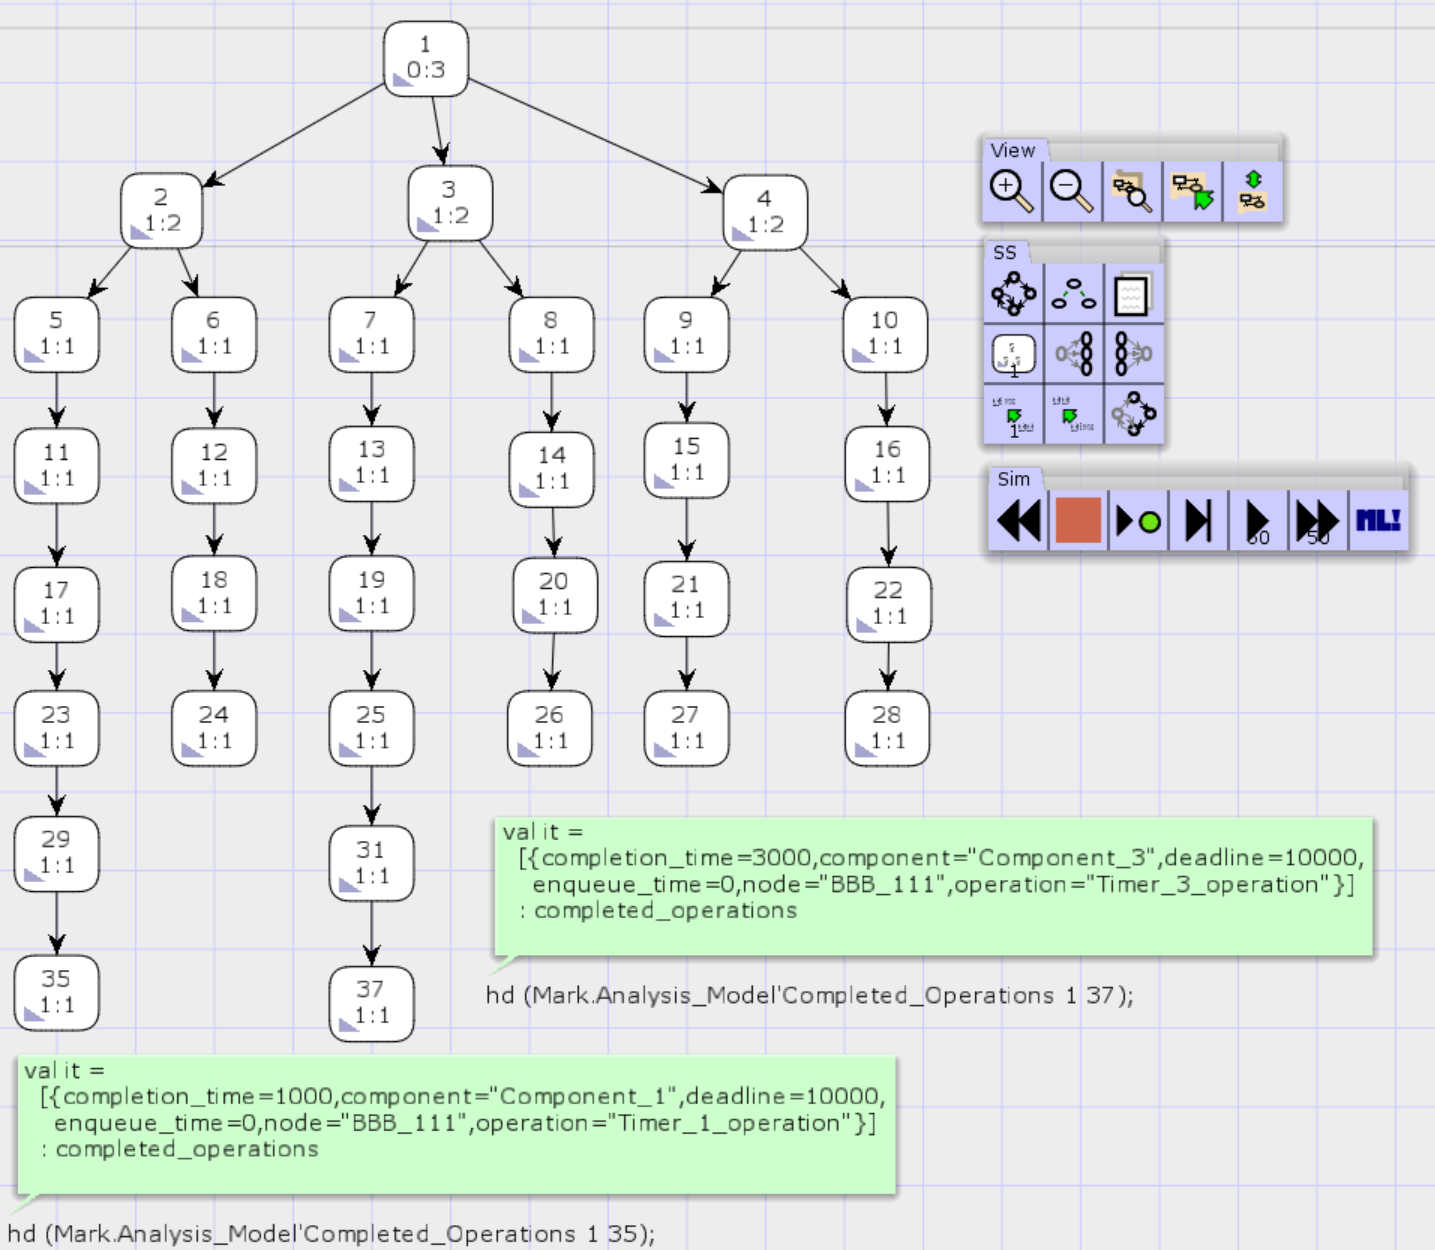
\includegraphics[width=\textwidth]{./img/state-space-analysis.png}
	\caption{Bounded State Space for a Multi-component Timer example -- The component threads have the same real-time priority and are executed in the same device. Each component is triggered with a 100 Hz periodic timer and all three timers are synchronized to illustrate non-determinism. The round robin  scheduling quantum is set to 4 milliseconds. 'Mark' is a state space query function that provides the \emph{marking} of a place in a particular state space node.}
	\label{fig:SSScreenshot}
\end{figure}
\FloatBarrier

\subsection{Searching the State Space}

CPNTools' inbuilt state space analysis tool comes with a programming interface -- a set of function that can be used by a user to query a generated state space. One of the many available functions is the \emph{SearchNodes} function, as shown in Figure \ref{fig:SSSearching}. This function traverses the nodes of the state space and at each node, evaluates a predicate and accumulates a list of nodes that satisfy this predicate. 

\begin{figure}[htb]
	\centering
	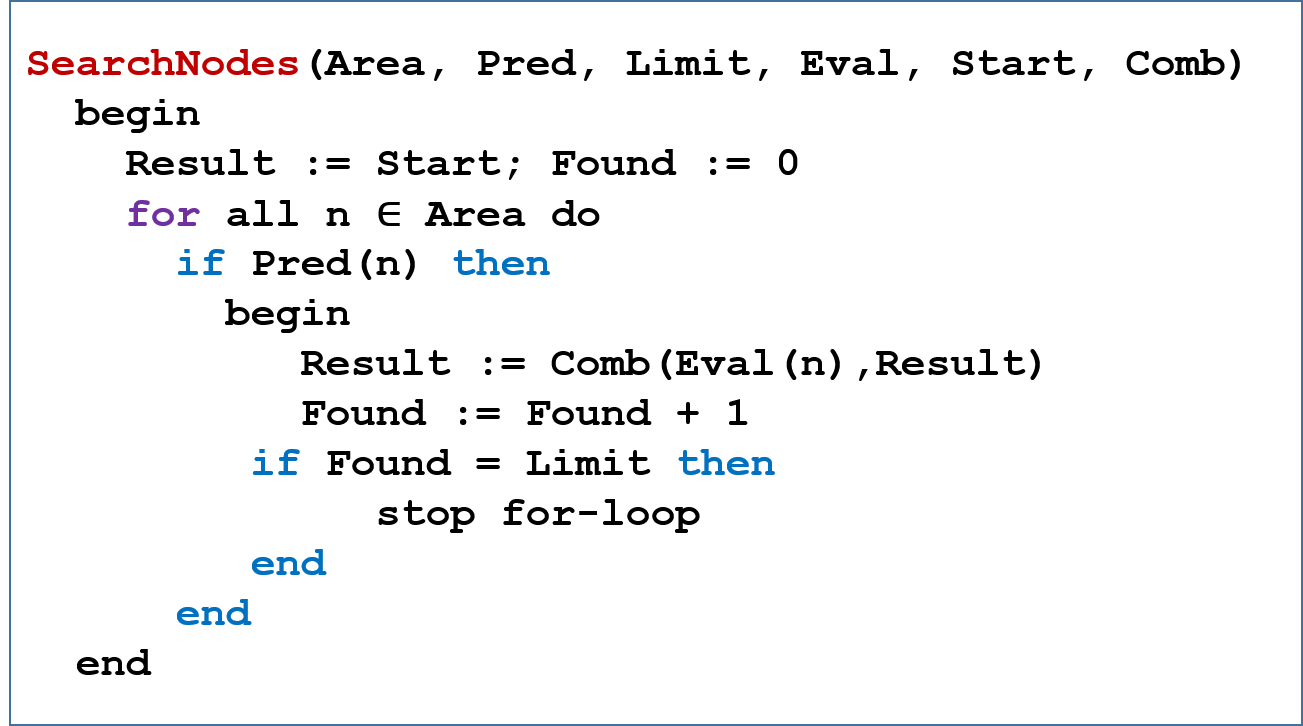
\includegraphics[width=0.7\textwidth]{./img/state-space-searching.png}
	\caption{SearchNodes function provided by CPNTools}
	\label{fig:SSSearching}
\end{figure}
\FloatBarrier

There are six parameters provided to this search function. \emph{Area} refers to the search area i.e. the part of the state space that needs to be searched. Often, the search area is the entire graph but it is possible to provide a subset of the graph e.g. a list of strongly connected components \footnote{A directed graph $G$ is strongly connected if every vertex is reachable from every other vertex in the graph. A strongly connected component is a maximal strongly connected subgraph of $G$ i.e. no additional edges or vertices from $G$ can be included in the subgraph without breaking its property of being strongly connected}. The second argument, emph{Pred}, specifies a predicate function that evaluates each node and produces a boolean result. All nodes that evaluate to false are ignored and all nodes that evaluate to true are retained for further analysis. The third argument, \emph{Limit} is an integer referring to how many times a predicate should evaluate to true before the search should terminate. If this limit is infinite, the entire state space is always searched. \emph{Eval} is an evaluation function that is executed on all state space nodes that satisfy the predicate function e.g. an evaluation function to find the execution time of an operation when its predicate function detects a deadline violation. Lastly, \emph{Start} is the initial value of the result and \emph{Comb} is a combination function that accumulates each new result from the evaluation function with prior results. The combination function is a constant time operation as it simply appends a new node to the end of the accumulated results list. The search algorithm itself has a time complexity of $O(n)$ where $n$ is the number of nodes in the state space. 

The rest of this chapter details how a bounded state space can be used to analyze DREMS applications for deadline violations, response times predictions etc. 

\subsection{Deadline Violations}

A \emph{deadline violation} refers to a system state where the execution time of a component operation has exceeded its deadline. The operation may violate its deadline without beginning execution since wait times in the message queue count towards the total delay from the arrival of the message to the completion of the corresponding operation. The SearchNodes function in CPNTools is quite generic and can be easily applied to our analysis model to identify such violations in the state space. For all operations, either completed or waiting for execution, it is sufficient to execute the predicate $current\_time - operation.enqueue_time > operation.deadline$. All nodes that satisfy this predicate are nodes that represent deadline violation states. 

Alternatively, by adding observer places to our timing analysis model i.e. places that passively observe the system and accumulate tokens when certain conditional transitions execute, deadline violations can be recorded as the model is executing. A \emph{Deadline\_Violation} (Figure \ref{fig:DL}) transition fires at any point in time when the guard \emph{dl\_guard} is satisfied and arc bindings are realized with its input places. The transition observes the states of the currently running threads and the component message queues to identify deadline violations on operations that are either executing or waiting to execute. The \emph{dl\_violation} tokens in \emph{Late Operations} ($LO$) is of the form:

\begin{equation}
\label{eq:DLV}
LO = \ <Node_{name}, O_{name}, O_{ST}, \ O_{DLT}>
\end{equation}

where operation $O_{name}$ executing on computing node $Node_{name}$ started at time $O_{ST}$ and violated its deadline at time $O_{DLT}$. Since the component-level scheduler uses a non-preemptive scheme, this operation is still run to completion after the violated deadline. Delays like these propagate to the waiting operations in the message queue.

\begin{figure}[htb]
	\centering
	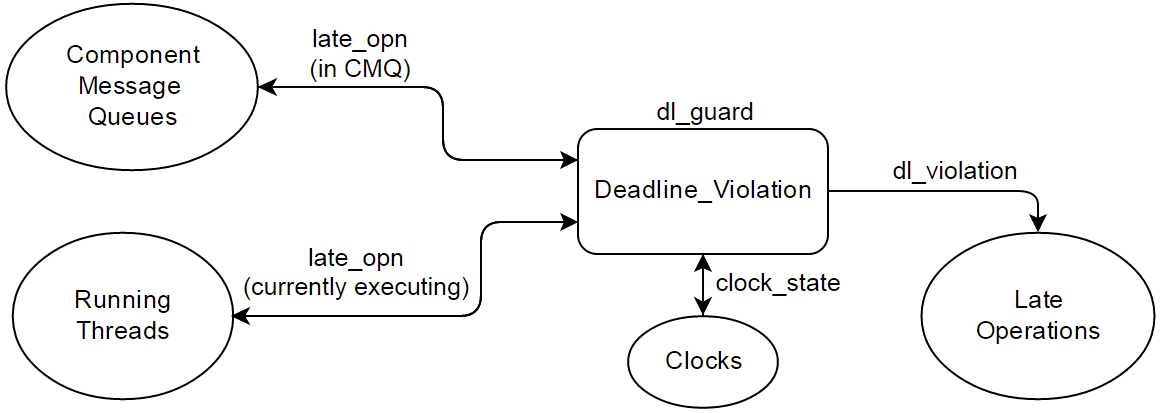
\includegraphics[width=\textwidth]{./img/Deadline_Violations.png}
	\caption{Deadline Violation Observer place}
	\label{fig:DL}
\end{figure}
\FloatBarrier

\subsection{System-wide Deadlocks}

System-wide deadlocks are caused by the inability of the OS schedulers (on all nodes) to schedule any component thread. This can be caused by situations where a set of executing threads are indefinitely blocked on each other because of cyclic dependencies in the interactions. Deadlocks can be identified by checking the leaf nodes of the bounded state space for \emph{dead transitions} that are unable to fire. Alternatively, the tokens in \emph{Component Interactions} are analyzed to identify cyclic dependencies and provide warnings to possible deadlocks. Such queries are useful in large component assemblies where mutually blocking dependencies are not immediately perceivable. 

\subsection{Response-time Analysis}

Response time analysis identifies the worst-case time taken for the system to generate a desired output signal after an input trigger has been provided e.g. time taken for the emergency braking system on an automated train controller to respond to sensory input. A component-based system can have a variety of triggers but in this context, a trigger is considered as any operation request received by a component. The response to this trigger is the completion of some other operation at a future time instant after the occurrence of the trigger. With state space analysis, it is possible to identify the worst-case response times for a $(trigger\_operation, response\_operation)$ pair by first obtaining response times for all trigger-to-response cycles and finding the maximum. 

Similar to deadline violation detection, using the SearchNodes function, this can be accomplished as follows -- The predicate function for the search is the completion of the response\_operation. The evaluation function scans the list of completed operations in all state space nodes where a response operation was the last operation marked as completed. In this list, by identifying the trigger operation and response operation, the response time is calculated as the difference $Response\_Operation_{cmpl\_time} - Trigger\_Operation_{enq\_time}$. This result is accumulated by the combination function and the maximum response time is calculated from the resultant list. The time complexity of this search is again linear with respect to the size of the state space. The size of the accumulated results list is at most half the size of the state space since the trigger and the response are always in separate state space nodes. Finding the maximum trigger-to-response time within the resultant list is also done in linear time.   

This result, as with other state space analysis results here, assumes ideal functional behavior for all operations i.e. the completion of the operation always provides the desired results. Since the business logic model for operations does not encode data-dependent behavior and conditional execution, the completion of a response operation is no indication about the correctness of the response, merely its timeliness. It is therefore also not possible to differentiate between response "types" as all responses are seen as equivalent. 

\subsection{Incomplete Designs}

As shown in Figure \ref{fig:SSScreenshot}, the state space generated by the timing analysis model contains all possible branches of execution from an initial system state. By encoding system requirements as predicates, it is possible to obtain useful analysis results that can aid system integrators in better designing components. When designing component-based systems, it is often the case where priorities need to be assigned to component threads executing on the same device, especially in real-time systems. These priorities are typically estimated based on relative importance of operations, order of component interactions, and frequency of associated triggers. An ideal priority assignment is one that leads to the most efficient schedule, one that avoids resource starvation while ensuring that the assignment does not violate any timing requirements. In large-sized component assembly, it is not always clear what each component's priorities should be. State space analysis can be useful here in providing a partial thread execution ordering based on the timing requirements of component operations. 

In Figure \ref{fig:SSScreenshot}, if the deadline i.e. timing requirement, of Timer\_1\_operation was 1 ms, then the thread ordering analysis would always suggest executing Component\_1 first before other components - essentially suggesting a higher priority for Component\_1 if this timing requirement is paramount. Furthermore, timing requirements can be ranked based on importance. A global timing requirement spanning distributed applications may be more important than a local timing requirement that is within the scope of a single component. To achieve this, the state space analysis identifies state space nodes where an operational timing requirement is satisfied and presents the order of thread execution on that device. By comparing such orderings with other ordering where such timing requirements fail, a system integrator obtains a partial execution order for threads. Using this result as feedback, the integrator can change the relevant component priorities and repeat the analysis. 


\section{Modeling and Analysis Improvements}
\label{sec:Improvements}

\subsection{Problem Statement}

The CPN analysis work presented in \cite{kumar2014colored} has some limitations. The clock values in the distributed set of computing nodes progress by a fixed amount of time regardless of the pace of execution. This is one of the primary causes of state space explosion since many of the intermediate states between \emph{interesting} events, though uneventful, are still recorded by the state space generation. For instance, in a temporal partition spanning 100 ms, even if a thread executes for 5 ms and the rest of the partition is empty, then if the clock progresses at a 1 ms rate, a 100 states are recorded in the state space when there are at most 5-7 interesting events in this interval. For a larger set of distributed interacting components, this can become a problem. Also, for distributed scenarios where multiple instance of a set of applications are executed in parallel, in independent computers, our CPN modeling methodology isn't efficient, leading to a tree of parallel executions even when the distributed computers are independent i.e. the computers can be synchronously progressed. The goal of this work is to mitigate such analysis issues and arrive at a more efficient and scalable analysis model. 

\subsection{Outline of Solution}
Improving the performance of our CPN analysis method required the evaluation of our existing results to identify how the state space generation worked. The state space of CPN is a tree of CPN \emph{markings}, where each marking is a data structure representing the tokens in all it's places. So, our goal is to reduce the number of markings accumulated in the CPN i.e. the number of distinct states of interest. This required us to evaluate our representation of time. Using time as a fixed-step monotonically increasing entity means that the CPN place managing time would always contain a new \emph{clock token}, therefore forcing the CPN marking to become a part of the state space.

To alleviate this issue, we modeled time as a dynamically changing variable, where the changes are strategically forced \emph{time jumps} instead of a statically increasing clock value. This is similar to a discrete event scheduling model but the next (closest) interesting event needs to be calculated based on the current state of the system. The states of all timers are used to calculate the next timer expiry. The states of all executing threads is evaluated to calculate the next closest preempt timestamp. Similarly, the state of all executing operations is analyzed to identify the next closest enqueue onto the component message queue. When temporal partitioning is enabled, the next partition switching timestamp is also considered in effectively calculating the minimum amount of time by which the analysis clock on each node needs to be progressed to ensure that time is efficiently managed while ensuring that no interesting event is \emph{skipped} because of the progression.

Similarly, our data structure representation for distributed deployments i.e. using unordered token sets instead of ordered lists, enabled our earlier CPN models to nondeterministically choose one of the various distributed nodes to execute, generating a exponentially increasing tree of execution orders. Once we moved to representing our distributed hardware nodes as a list, the execution engine iteratively executing the analysis on each node in the list, leading to one execution order instead of a tree. 

Such issues are resolved with our analysis improvements, reported in \cite{SEUS}. We modified the timing analysis model to allow dynamic time progression i.e. the clocks (one for each computing node) in the CPN model do not progress at a constant rate but instead experience \emph{time jumps} to the next interesting time step e.g. next timer expiry, end of partition, next scheduling preemption point, or next remote interaction. This makes the system execution progress at a much higher rate and reduces the overall number of states being recorded in the state space. We also adjusted our modeling concepts when describing distributed deployments. We experienced needless state space explosions as a consequence of using CPN semantics when modeling distributed computers. If the computers are modeled as an aggregate of independent CPN tokens, then the CPN transition that progresses the execution in each computer is independent, leading to a potential $C!$ different orders for $C$ computers. For instance, 4 distributed computers leads to 24 possible execution orders displayed by the transition responsible for \emph{picking} the next computer to evaluate and progress. We alleviate this issue by assuming that all computers in a distributed scenarios have synchronized clocks and execute simultaneously leading to a synchronous progress. In practice this can be achieved by using the Precision Time Protocol (PTP) \cite{correll2005design} to synchronize clocks throughout the computer network. In CPN, this is done by maintaining the state of each computer in a \emph{list} instead of an unordered aggregate. 

\subsection{Handling Time}
\label{handling_time}

The CPN-based analysis consists of executing a simulation of the model and constructing a state space data structure for the system (for a finite horizon), and then performing queries on this data structure. This is automated by CPN Tools. The first improvement over the basic CPN approach is in how we handle time. Although it is true that CPN and similar extensions to Petri Nets such as Timed Petri Nets inherently have modeling concepts for simulation time, we explicitly model time as an integer-valued \emph{clock} color token in CPN. There are several reasons for this choice. 

Firstly, this is an extension to our previous arguments about choosing Colored Petri Nets. Modeling the OS scheduler clock as a colored token allows for extensions to its data structure such as (1) intermediate time stamps and internal state variables, and (2) adding temporal partitioning schemes like the (time-partitioned) ARINC-653 \cite{ARINC-653} scheduling model (Figure \ref{fig:clock}). 

\begin{figure}[h]
	\centering
	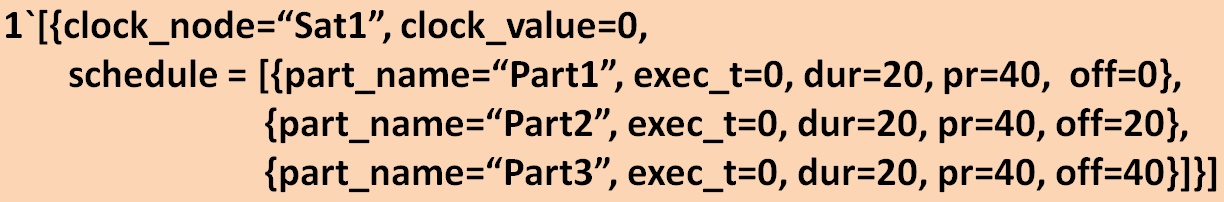
\includegraphics[width=\textwidth]{./img/clock}
	\caption{A Clock Token with Temporal Partitioning}
	\label{fig:clock}
\end{figure}

These extended data structure fields can be more easily manipulated and used by the model transitions during state changes, allowing for richer modeling concepts that would not be easily attainable using token representations provided by Timed Petri Nets. The ability to pack colored tokens with rich data structures also reduces the total number of colors required by the complete model. This quantitative measure directly influences the reduced size of the resultant state space. The downside of this approach to modeling is that we have to choose a time quantum. But in practical systems this is usually not a problem, as the low-level scheduling decisions are taken by an OS scheduler based on a time scale with a finite resolution. 

Secondly, modeling time as a token allows for smarter time progression schemes that can be applied to control the pace of simulation. If we did not have such control over time, the number of states recorded for this color token would eventually explode and itself contribute to a large state space. In order to manage this complexity, we have devised some appropriate \emph{time jumps} in specific simulation scenarios. 

If the rate at which time progresses does not change, then for a 1 msec time resolution, \emph{S} seconds of activity will generate a state space of size: $SS_{size} = \sum\limits_{i=1}^{S*1000} TF_{t_i}$ where $TF_{t_i}$ is the number of state-changing CPN transition firings between $t_i$ and $t_{i+1}$. This large state space includes intervals of time where there is no thread activity to analyze either due to lack of operation requests, lack of ready threads for scheduling, or due to temporal partitioning. During such idle periods, it is prudent to allow the analysis engine to \emph{fast-forward} time either to (1) the next node-specific clock tick, (2) the next global timer expiry event, or (3) the next activation of the node-specific temporal partition (whichever is earliest and most relevant). This ensures that the generated state space tree is devoid of nodes where there is no thread activity.

\begin{figure}[h]
	\centering
	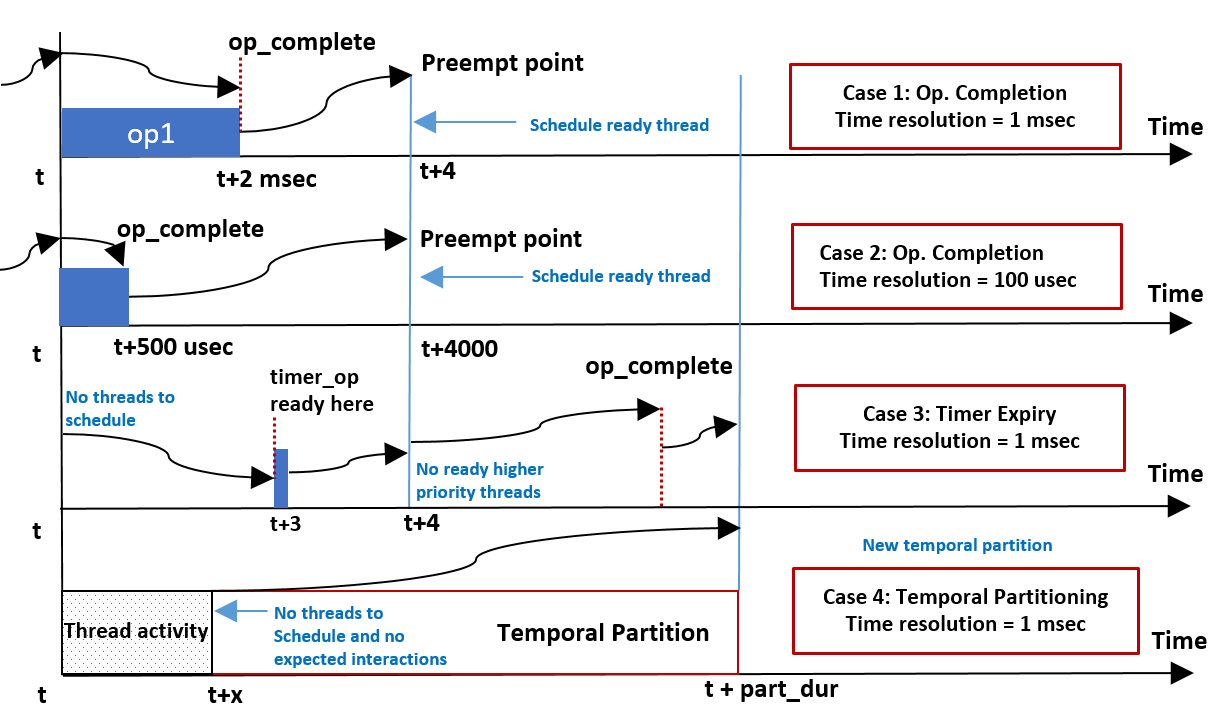
\includegraphics[width=\textwidth]{./img/time}
	\caption{Dynamic Time Progression}
	\label{fig:time}
\end{figure}

Figure \ref{fig:time} illustrates these time jumps using 4 scenarios. Assuming the scheduler clock ticks every 4 msec, Case 1 shows how time progression is handled when an operation completes 2 msec into its thread execution. At time t, the model identifies the duration of time left for an operation to complete. If this duration is earlier than the next preemption point, then there is no need to progress time in 1 msec increments as no thread can preempt this currently running thread till time t + 4 msec. Therefore, the \emph{clock\_value} in Figure \ref{fig:clock} progresses to time t + 2 msec, where the model handles the implications of the completed operation. This includes possibly new interactions and operation requests triggered in other components. Then, time is forced to progress to the next preemption point where a new candidate thread is scheduled. This same scenario is illustrated in Case 2 when the time resolution is increased to 100 usec instead of 1 msec. Notice that the number of steps taken to reach the preemption point are the same, showing how the state space doesn't have to explode simply because the time resolution is increased. Case 3 illustrates the scenario where at time t, the scheduler has no ready threads to schedule since there are no pending operation requests but at time t + 3 msec, a component timer expires, triggering an operation into execution. Since timers are maintained in a global list, each time the \emph{Progress\_Time} transition checks its firing conditions, it checks all possible timers that can expiry before the next preemption point. So, at time t when no threads are scheduled, the model immediately jumps to time t + 3. This scenario also shows that if the triggered operation does not complete before the preemption point \emph{and} there are no other ready threads or timer expiries that can be scheduled, the clock value jumps to the operation completion. It must be noted here that this case is valid only because the DREMS architecture we have considered uses a non-preemptive operation scheduling scheme. Lastly, Case 4 shows time jumps working with temporal partitioning. At some time t + x, the model realizes the absence of ready threads and does not foresee any interaction requests from other components, then it safely jumps to the end of the partition without stepping forward in 1 msec increments. This time progression directly shows how the state space of the system execution reduces while still preserving the expected execution order, justifying our choice of modeling time as a colored token using CPN. 

\subsection{Distributed Deployment} 
\label{distributed_deployment}

The second structural change to the analysis model is in how distributed deployments are modeled and simulated. Early designs on modeling and analysis of distributed application deployments \cite{kumar2014colored} included a unique token per CPN place for each hardware node in the scenario. Since the individual \emph{node} tokens are independent and unordered, there is nondeterminism in the transition bindings when choosing a hardware node to schedule threads in. For instance, if there are 2 hardware nodes in the deployment with ready threads on both nodes, then either node can be chosen first for scheduling threads leading to two possible variations of the model execution trace. Therefore the generated state space would exponentially grow for each new hardware node. In order to reduce this state space and improve the search efficiency, we have merged hardware node tokens into a single \emph{list} of tokens instead of a unassociated grouping of individual node tokens. This approach is inspired by the symmetry method for state space reduction \cite{Kristensen2000}.

\begin{figure}[h]
	\centering
	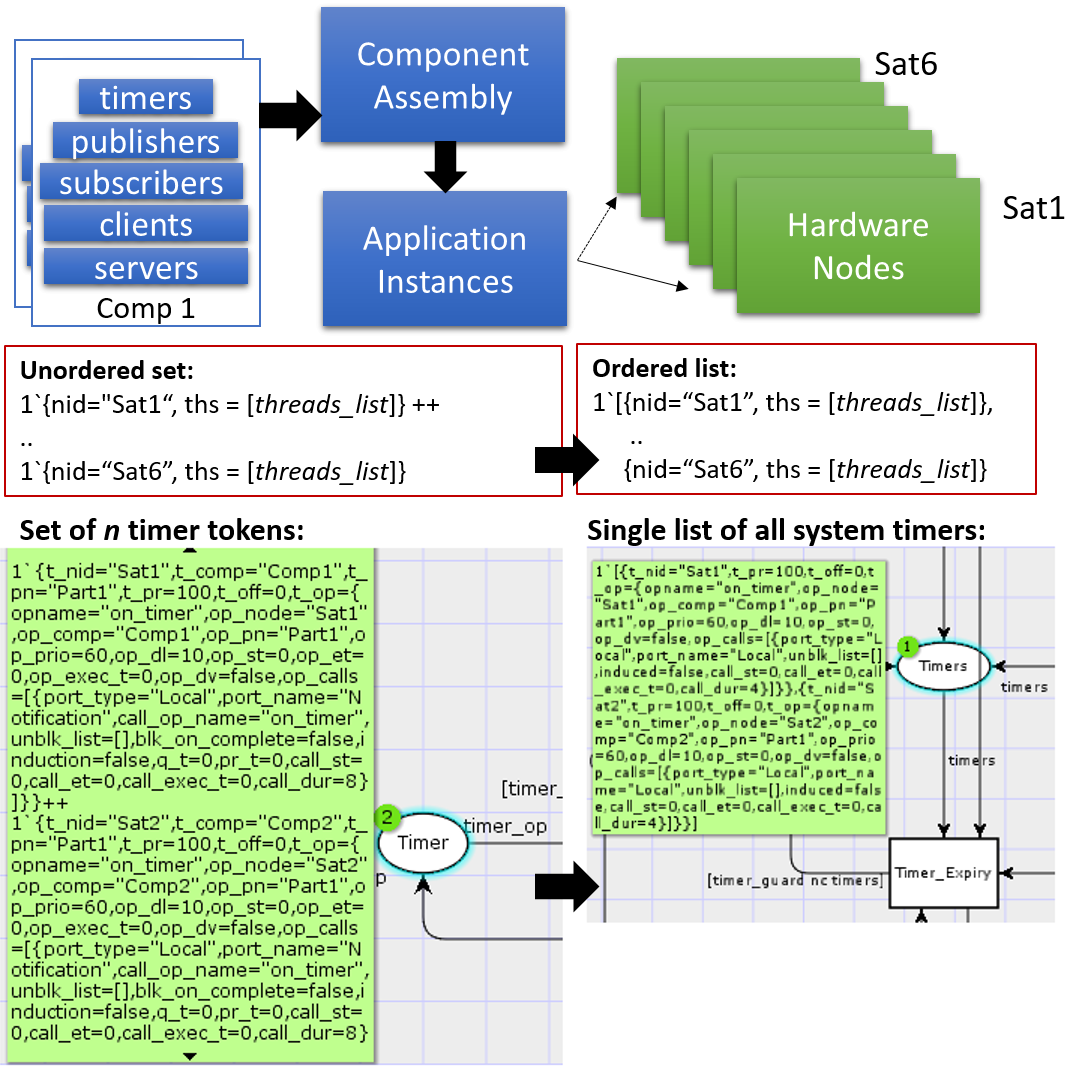
\includegraphics[width=0.8\textwidth]{./img/dd}
	\caption{Structural Reductions in CPN}
	\label{fig:dd}
\end{figure}

Figure \ref{fig:dd} illustrates this structural reduction. Consider a distributed deployment scenario with an instance of a DREMS application deployed on each hardware node, Sat1 through Sat6. Components \emph{Comp1} and \emph{Comp2} are triggered by timers, eventually leading to the execution of component operations (modeled as shown in Figure \ref{fig:ebnf}). If all the timer tokens in the system were modeled individually, the transition \emph{Timer\_Expiry} would non-deterministically choose one of the two timer tokens that are ready to expire at \emph{t=0}. However, if the timers are maintained as a single list, then this transition (1) consumes the entire list, (2) identifies all timers that are ready to expire, (3) evaluates the timer expiration function on all ready timers, (4) propagates the output \emph{operation} tokens to the relevant component message queues in a single firing. This greatly reduces the tree of possible transition firings and therefore the resultant state space. Also, if there is no non-determinism in the entire system, i.e., there is a distinct ordering of thread execution, then this model can be scaled up with instantiating the application on new hardware nodes with no increase in state space size. This is because all of the relevant tokens on all nodes are maintained as a single list that is completely handled by a single transition firing. 

An important implication of the above structural reduction is that the simulation of the entire system now progresses in synchronous steps. This means that at time 0, all the timers in all hardware nodes that are ready to expire will expire in a single step. Following this, all operations in all component message queues of all these nodes are evaluated together and appropriate component executor threads are scheduled together. When these threads execute, time progresses as described in Section \ref{handling_time}, moving forward by the minimum amount of time that can be fast-forwarded.

\newpage
\section{Investigating Advanced State Space Analysis Methods}

\subsection{Problem Statement}
State space analysis techniques have been successfully applied with Colored Petri Nets in a variety of practical scenarios and industrial use cases \cite{CPN_0}, \cite{CPN_1}. The basic idea here is to compute all reachable states of the modeled concurrent system and derive a directed graph called the state space. The graph represents the tree of possible executions that the system can take from an initial state. It is possible from this directed graph to verify behavioral properties such as queue overflows, deadline violations, system-wide deadlocks and even derive counterexamples when arriving at undesired states. 

Advanced state space analysis techniques arise from the need for efficient space space searching algorithms. State space analysis is challenged by time, memory, and computational power. Large state spaces require large CPU RAM and efficient search methodologies to quickly arrive at a useful result. With increasingly complexity in system designs, the number of state variables to store in memory also increases. Our problem here is to identify and apply advanced state space analysis techniques, applicable in the context of our CPN model and available as tested analysis tools that mitigate such complexities in state space analysis. This will help improve the scalability of our model and also reduce the memory footprint of the analysis. 

\subsection{Outline of Solution}

The variety of CPN-specific state space reduction techniques \cite{CPN_Sweepline}, \cite{CPN_Symmetry} developed in recent times has significantly broadened the class of systems that can be verified. In order to easily apply such techniques to our analysis model, we use the ASAP \cite{ASAP} analysis tool. The tool provides for several search algorithms and state space reduction techniques such as the \emph{sweep-line method} \cite{Christensen2001} which deletes already visited state space nodes from memory, forcing on-the-fly verification of temporal properties. The main advantage of such techniques is the amount of memory required by the analysis to verify useful properties for large models. 

The sweep line method for state space reduction is used to check for important safety properties such as lack of deadlocks, timing violations etc. using user-defined model-specific queries. Practical results enumerated in \cite{Christensen2001} show improvements in time and memory requirements for generating and verifying bounded state spaces. The method relies of discarding generated states on-the-fly by performing verification checks during state space generation time. Any state that does not violate system properties can be safely deleted. Another advantage of this method compared to similar reduction methods such as bit-state hashing \cite{CPN_Bitstate_Hashing} is that a complete state space search is guaranteed. 

\subsection{Evaluation of Solution}
We have evaluated these advanced state space analysis methods by comparing the obtained results with our basic state space analysis in CPN Tools. Using several criteria such as state space generation time, state space query generation, query processing time, memory usage etc., we can generate a comparison table to show the overall improvements in the analysis workflow. Advanced analysis techniques are usually accompanied by some expertise requirements that can be masked by nicely designed analysis tools. Our goal with ASAP is to use a model-driven approach to enable advanced analysis methods that does not require much expertise. With ASAP, we are able to generate verification project templates i.e. building blocks much like Simulink that are wired up together and provide an interface to the low-level analysis engine. Therefore, evaluation of this work requires both the evaluation of the advanced methods applied, and the tool used. As for the analysis methods applied, it is important to ensure that the state space tree, with all of the applied analysis heuristics, is still sufficiently probed when searching for system properties. Heuristics that enable state space analysis but only by partially checking the tree can lead the case where the state space analysis does not identify timing errors because of the incomplete search. This will be checked with negative test cases where the design model is known to be flawed; if the results from ASAP identify injected timing errors for all test cases, then the analysis is sound. 

\subsection{Contributions}
These methods were evaluated on our CPN analysis method and the results were presented in \cite{SEUS}. We used a large and diverse 100 component-based application for our testing. Using the CPN Tools' built-in state space analysis tool, a bounded state space of thread activity was generated. The state space generation took 36 minutes on a typical x86 laptop. We imported the same CPN analysis model onto ASAP and performed on-the-fly verification checks for lack of dead states in the analysis model for the same bounded state space. The on-the-fly verification, without any graphical interface overheads, took less than 10 minutes to compute a lack of system-wide deadlocks. It must be noted here that this improved result is due to not only because of the efficient state space search but also because of symmetry-based structural reduction discussed in the previous section.

In order to illustrate the utility of such state space reduction techniques, we consider a large-scale deployment. Figure \ref{fig:gm} shows the generated CPN model for a domain-specific DREMS application. This is a scaled-up variant of several satellite cluster examples we have used in previous publications \cite{DREMS13Software, kumar2014colored}. The example consists of a group of communicating satellites hosting DREMS applications. The component assembly for this application consists of 100 interacting components distributed across 10 computing nodes, many of which are triggered by infrastructural timers. Notice in Figure \ref{fig:gm} how there is only one token in each of the main CPN places, as described in Section \ref{distributed_deployment}. All of the component timers are appended to the list maintained in \emph{Timers} place. Similarly, all node-specific clock tokens are maintained in place \emph{Clocks}.  

\begin{figure}[h]
	\centering
	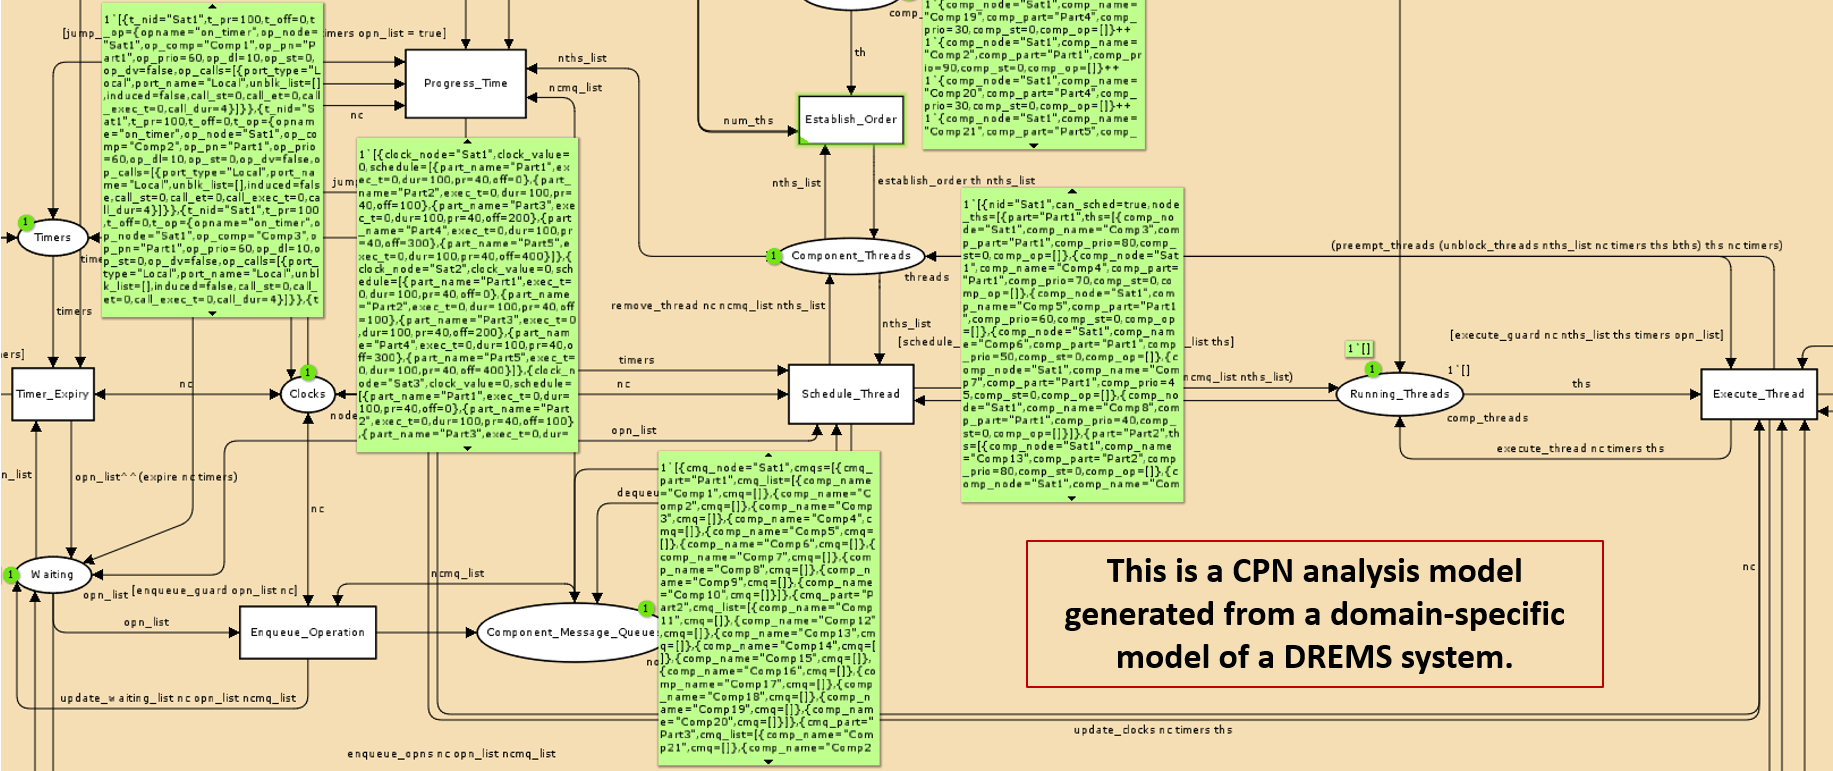
\includegraphics[width=\textwidth]{./img/Generated_Model}
	\caption{Generated CPN model for a Distributed Application Deployment}
	\label{fig:gm}
\end{figure}

At time \emph{t=0}, before the simulation is kicked off, the transition \emph{Establish\_Order} generates the powerset of thread execution orders that are possible given the configuration of the clock token. This may be a potentially large set depending on the number of threads of equal priority in each partition. Once this tree of possible orders is established, the complete set of timers that are ready to expire are evaluated. Each timer expiry manifests as an operation request and each callback operation modeled using the grammar shown in Figure \ref{fig:BL_Model}. Once the operations are ready to execute, the highest priority component thread with a pending operation request is chosen for execution. This thread scheduling happens on all hardware nodes. When each thread executes, new interactions may occur as a consequence of the execution. For instance, if a component thread executes a timer operation in which the component publishes on a global topic, the consequence of this action would include a set of callback operation requests on all components that contain subscribers to that global topic. Lastly, all running threads are evaluated to identify the minimum amount of time that can be safely fast-forwarded in each node. If the running component threads are independent or symmetrical, then the maximum possible time progression is up to the end of the temporal partition. Note here that temporal partition in the deployment can be set to an empty list which simply removes the  partitioning constraint and treats all component threads on a node as candidate threads for execution. The above sequence of transitions repeat for as long as there is a timer expiry, a pending operation request or an unfinished component interaction. 

\begin{figure}[h]
	\centering
	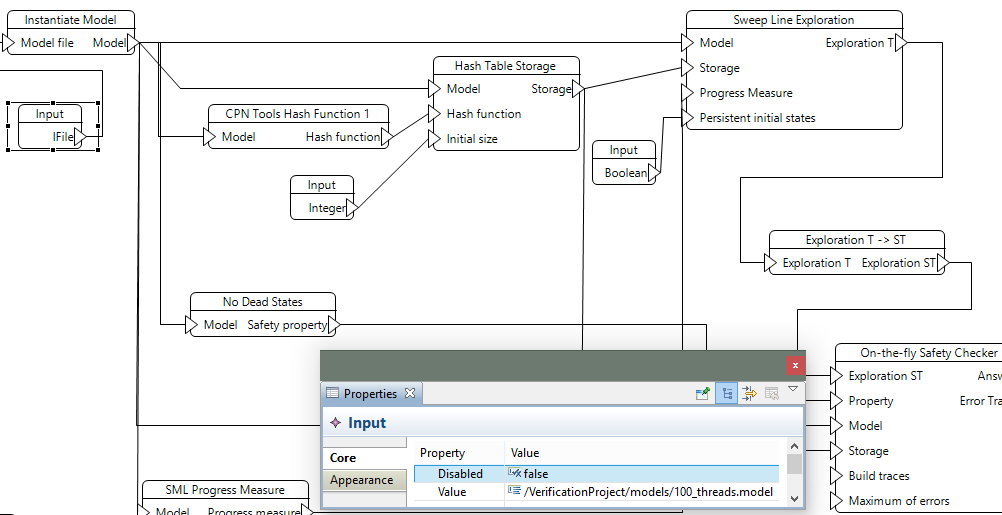
\includegraphics[width=\textwidth]{./img/sl}
	\caption{Sweep-Line Method}
	\label{fig:sl}
\end{figure}

Using the CPN Tools' built-in state space analysis tool, a bounded state space was generated reaching up-to 20 hyperperiods of component thread activity. This bounded generation took 36 minutes on a typical laptop. Our goal with such an example is to evaluate the effectiveness and utility of state space reduction techniques with respect to speed and memory usage. Figure \ref{fig:sl} shows a simple block diagram of the sweep-line method as configured in ASAP. Performing on-the-fly verification checks for lack of dead states in the analysis model, results indicate lack of system-wide deadlocks due to blocking behaviors triggered by RMI-style synchronous peer-to-peer interaction patterns. Figure \ref{fig:ds} shows analysis results obtained from a \emph{Verification Job} executed in the tool. Notice the on-the-fly verification taking less than 10 minutes to perform deadlock checks on this sample deployment. Using the \emph{Palette} in ASAP, several standard ML (SML) user queries can be created to check for domain-specific properties. 

\begin{figure}[h]
	\centering
	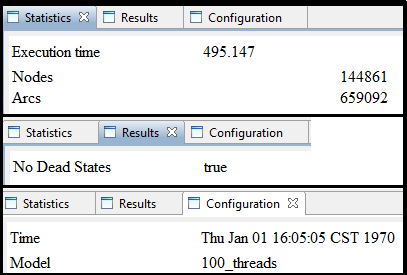
\includegraphics[width=0.6\textwidth]{./img/asap}
	\caption{Dead States Checking in a Component-based application}
	\label{fig:ds}
\end{figure}

It must be noted here that this improved result is due to not only because of the efficient state space search but also because of symmetry-based structural reduction discussed in the previous section. If not for this reduction, the state space search requirements would exponentially grow for each new hardware node added to the deployment. 
% Describe RCPS Testbed & Testing Platform
% Describe evaluation metrics
% Describe testing scenarios and use cases
\chapter{Experimental Evaluation}
\label{chapter:evaluation}

Experimentally validating our timing analysis results is an important and necessary requirement. In order to obtain any level of confidence in our CPN-based work, the system design model needs to be completed implemented, and deployed on the target hardware platform. We have constructed a testbed \cite{kumarTestbed} to simulate and analyze resilient cyber-physical systems consisting of 32 Beaglebone Black development boards \cite{BBB}. We have chosen the light-weight ROS \cite{ROS} middleware layer and implemented our ROSMOD Component model \cite{kumarROSMOD} on top of it. This component model provides the same execution semantics and interaction patterns as our DREMS component model \cite{ISIS_F6_ISORC:13}. Our goal with this work is to (1) establish a set of distributed component-based applications, (2) translate this design model to our CPN analysis model, (3) deploy these applications on our testbed and accurately measure operation execution times, and finally (4) perform state space analysis on the generated CPN model to check for conservative results, compared against the real system execution.

\subsection{Challenges}

Experimental validation requires that online measurements of the real-time system match with the design-time timing analysis results in a way that the timing analysis results are always close but conservative. If the timing analysis results predict a deadline violation, this does not necessarily mean that the real system will violate deadlines but if the timing analysis and verification guarantees a lack of deadline violations, then the real system should follow this prediction. The design-time timing analysis primarily uses bounded state space analysis for such predictions. The analysis is bounded by necessity i.e. to tackle the state space explosion problem. Obtaining confidence from the timing analysis results depends entirely on the behavior of the system and the applied bounds. Recall that DREMS components are dormant by nature and need to be triggered either by timers or through interaction ports. Component-based applications using DREMS typically exhibit some periodic behavior i.e. sequences of interactions between components that repeats periodically. Each interaction sequence could involve a set of distributed components or assemblies. In such scenarios, design-time analysis bounds the state space generation to some constant multiple of the overall period of the application. The overall period here is some duration of time after which all of the sequences of interactions in the application have repetition. By analyzing some reasonably large multiple of the application period, the state space analysis both generates and searches a sufficiently large set of states of the system i.e. execution behaviors. Assuming the execution correctness of the timing analysis model and sufficiently conservative worst-case estimates of execution times, a complete absence of timing anomalies in this bounded state space is typically a good indication of a safely executing system. There are various ways to obtain the WCET values for individual operational steps but the easiest approach is to execute the design on our testbed and make accurate measurements.

%You also need to come up with a 'worst-case' input for the operation, as well as have to run a lot of experiments and compute the WCET from the data. 

WCET of component operational steps needs to be measured by having the component operation execute at highest priority with no other component threads intervening this process. Secondly, this experiment must be repeated multiple times with different inputs (if any), including the worst-case input. The worst-case measurement across multiple runs of the experiment gives us a \emph{pure execution time} of the code block. 

Obtaining the WCET values by this method is not only more realistic but also an accurate representation of the target system. Once these individual numbers are obtained, the values are plugged into the CPN through our business-logic models. Ideally, the CPN model, consisting of a composition of component operation models, when analyzed, produces results that closely resemble a real-system deployment of the component assembly. Such results would validate the modeling accuracy and the analysis results.

%Distributed CPS are hard to develop hardware/software for; because the software is coupled with the hardware and the physical system, software testing and deployment may be difficult - a problem only exacerbated by distributing the system.  These types of systems must be tested for performance assurances, reliability, and fail-safety.  Examples of these systems include UAV/UUV systems, fractionated satellite clusters, and networks of autonomous vehicles, all of which require strict guarantees about not only the performance of the system, but also the reliability of the system.  Because of the need for such strict design-time guarantees, many traditional techniques for software testing cannot be used.  Cloud-based software testing may not accurately reflect the performance of the software, since many of these systems use specialized embedded computers, and furthermore does not provide the capability to easily integrate a system simulation into the software testing loop.  For such systems, a closed-loop simulation testbed is necessary which can fully emulate the deployed system, including the physical characteristics of the nodes, the network characteristics of the systems, and the sensors and actuators used by the systems.

%Emerging industry standards and collaborations are progressing towards component-based system development and reuse, \emph{e.g.} AUTOSAR~\cite{autosar} in the automotive industry.  As these systems are becoming increasingly more reliant on collections of software components which must interact, they enable more advanced features, such as better safety or performance, but as a consequence require more thorough integration testing.  Comprehensive full systems integration is required for system analysis and deployment, and the development of relevant testing system architectures enables expedited iterative integration.  Developing these systems iteratively, by prototyping individual components and composing them can be expensive and time consuming, so tools and techniques are needed to expedite this process.  Our testbed architecture was developed to help address these issues and decrease the turn-around time for integration testing of distributed, resilient CPS.  

%Examples of such systems which can be prototyped and tested using this architecture are (1) autonomous cars, (2) controllers for continuous and discrete manufacturing plants, and (3) UAV swarms.  Each of these systems is characterized as a distributed CPS in which embedded controllers are networked to collectively control a system through cooperation.  Each subsystem or embedded computer senses and controls a specific aspect of the overall system and cooperates to achieve the overall system goal.  For instance, the autonomous car's subsystems of global navigation, pedestrian detection, lane detection, engine control, brake control, and steering control all must communicate and cooperate together to achieve full car autonomy.  The control algorithms for each of these subsystems must be tested with their sensors and actuators but also must be tested together with the rest of the systems.  It is these types of cooperating embedded controllers which are a distinguishing feature of distributed CPS.  Integration testing for these distributed CPS can be quickly and easily accomplished using hardware-in-the-loop simulation, but must accurately represent the real physical system, hardware, software, and network. 

%In scenarios like the automotive networked CPS, one of the main challenges with system testing is the discord between the standardized networking protocols and communication methods e.g. CAN bus, and the manufacturer-specific implementations of these methods. It is difficult to obtain public access to the implementation details for such interaction patterns and therefore pure simulation of the communication protocols using event-simulation tools  is not sufficient in validating resilient application performance. The comprehensive testing for such safety-critical systems require \emph{replicating the CPS} by using a testing infrastructure that provides similar hardware and executes the exact embedded control code that would execute on the final system. 

% Section on our RCPS Testbed
\section{Resilient Cyber-Physical Systems (RCPS) Testbed}

\subsection{Architecture}

The testbed consists of 32 \emph{RCPS nodes}, each of which is a Beaglebone Black (BBB) \cite{BBB} development board. We execute a full software stack including a ROS-based middleware, called ROSMOD \cite{kumarROSMOD} and the DREMS component model. For the subset of CPS we are interested in, the behavior of the CPS can be much more precisely emulated with these boards compared to running the applications inside of a standalone simulation. For example, NASA's CubeSat Launch Initiative (CSLI) \cite{CubeSat} provides opportunities for nanosatellites to be deployed into space for research. CubeSats are small (4-inch long) satellites running low-power embedded boards and being prepared for interplanetary missions \cite{CubeSat_Mars} to Mars. A distributed set of CubeSats can be easily tested with this architecture if it can be integrated with a high-fidelity space flight simulator.  

\begin{figure}[h]
    \centering
    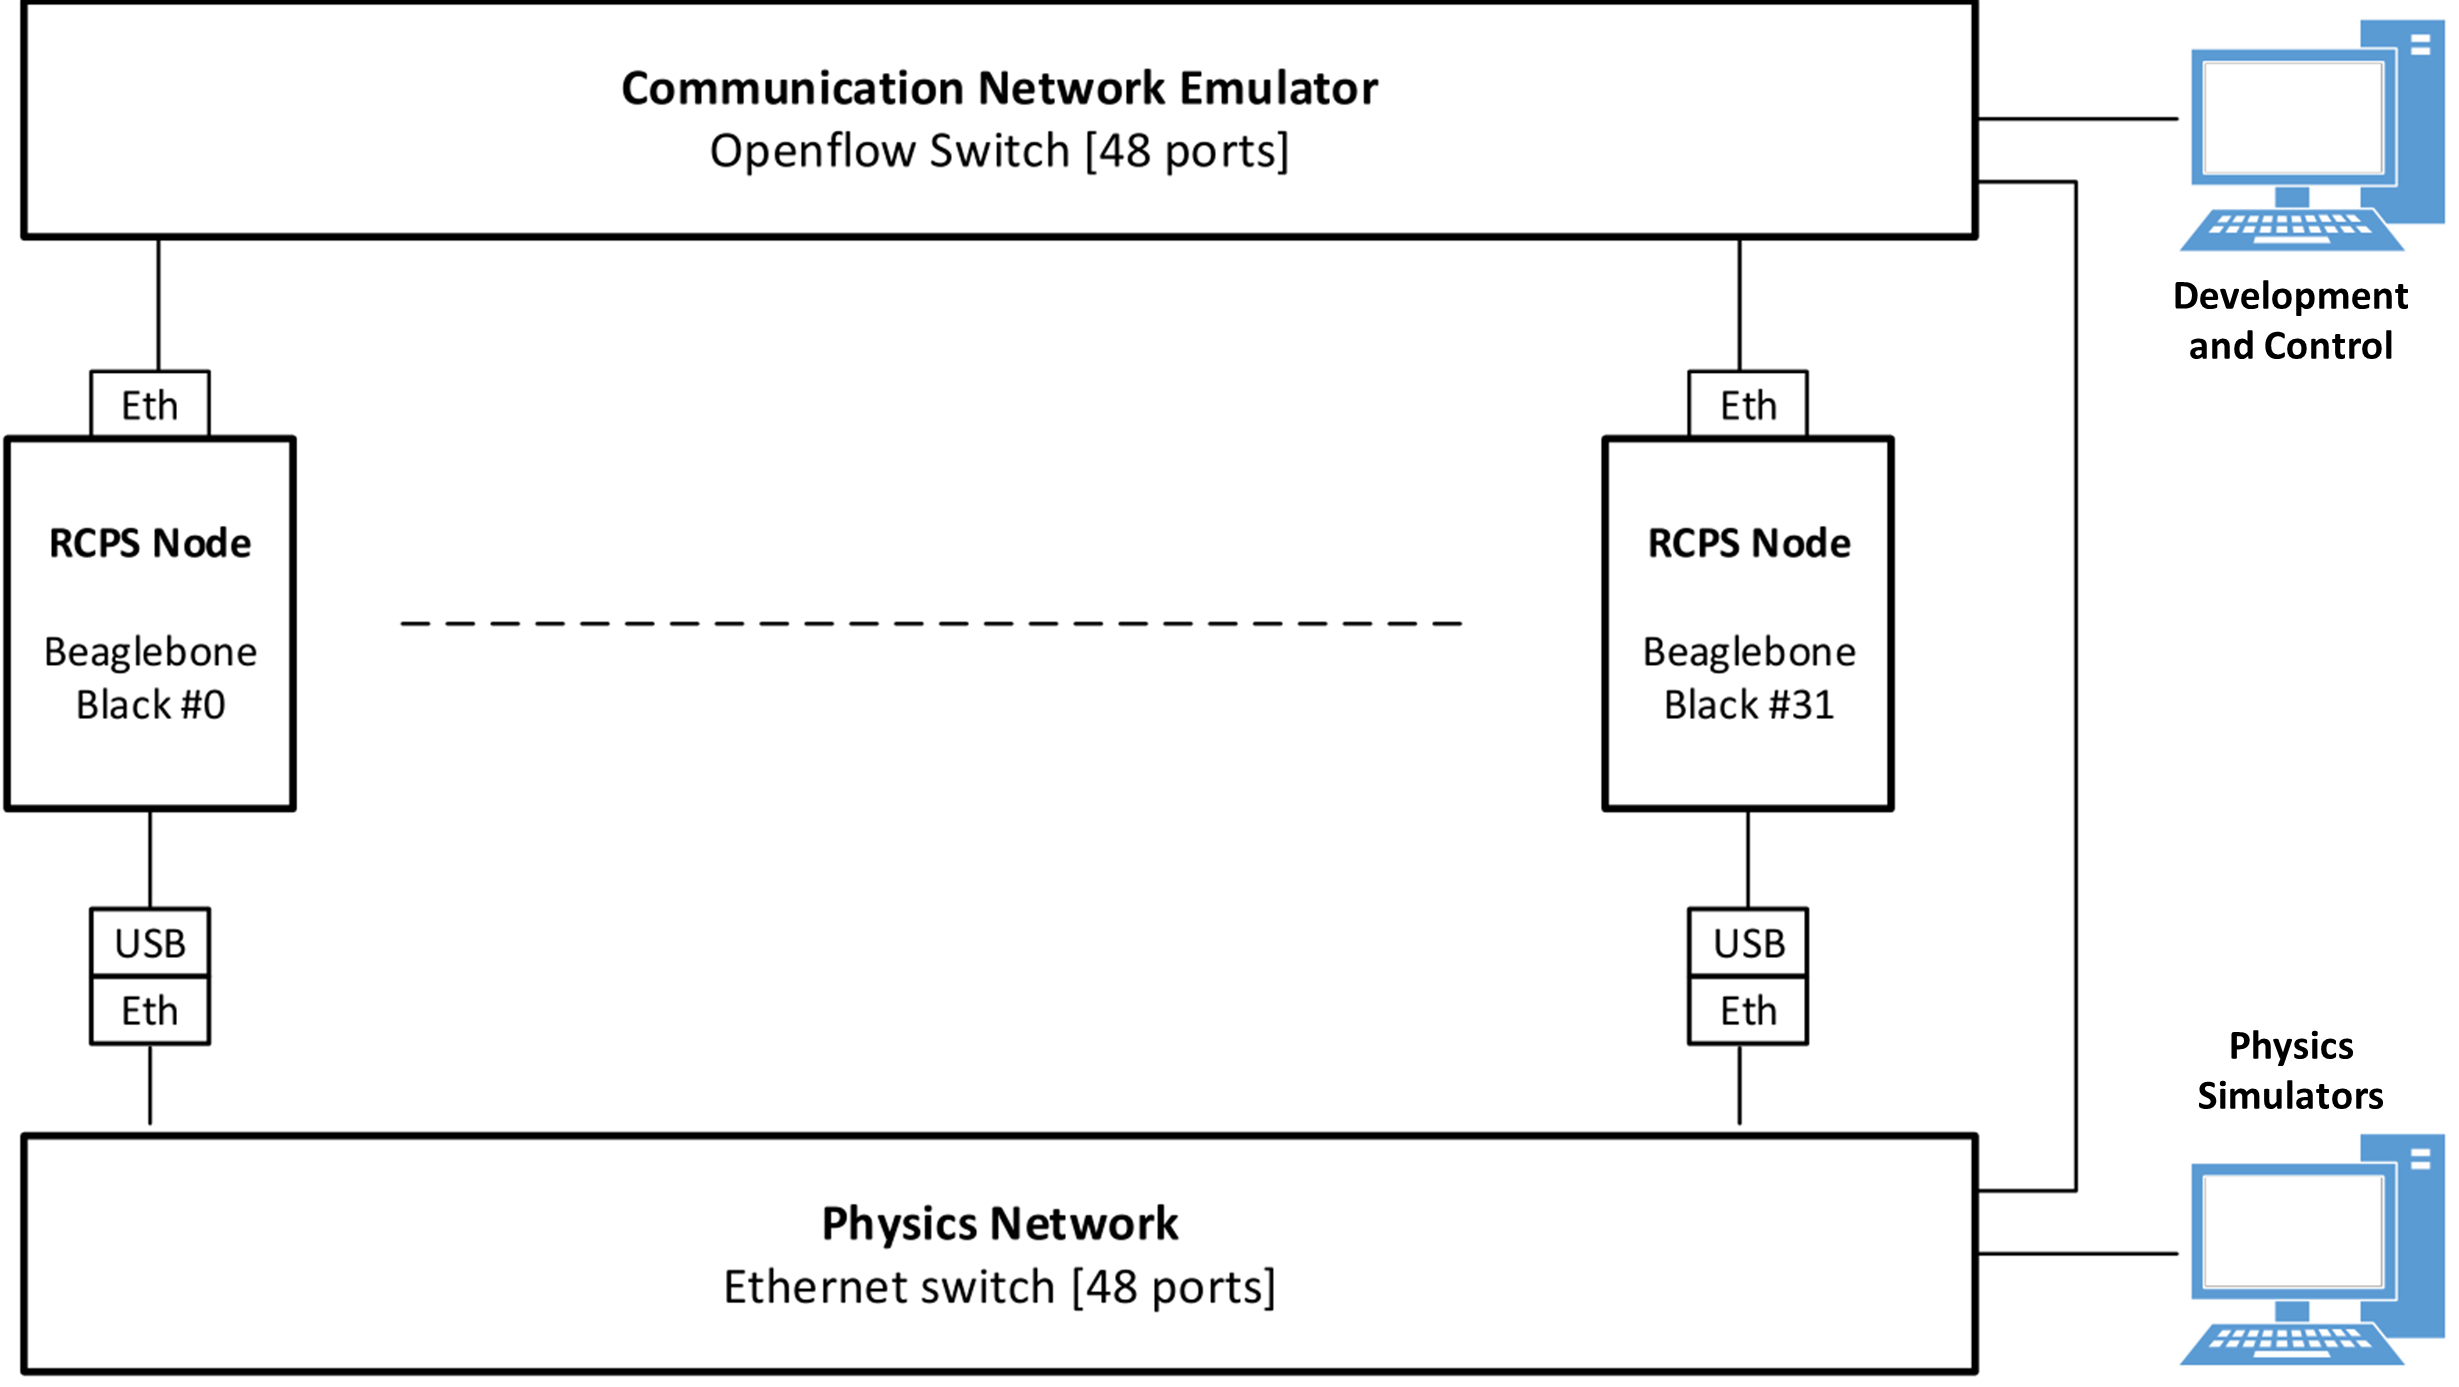
\includegraphics[width=\textwidth]{rcps-architecture.png}
    \caption{Testbed Architecture}
    \label{fig:architecture}
\end{figure}

The Gigabit Ethernet port of each BBB is connected to a \emph{Communication Network} switch. This is a programmable OpenFlow \cite{openflow} switch, allowing users to program the flowtable of the switch to control the routes that packets follow and completely configure the full network and subnets required for their emulated deployment.  Furthermore, the configurability of the communications network enables per-link or per-flow bandwidth throttling, enabling precise network emulation.  The primary \emph{Development and Control} machine, running our software development tools, communicates with the BBBs using this network. After software applications are deployed on this testbed, the characteristics of the real CPS network can be enforced on the application network traffic. Therefore, this network emulates the physical network which a distributed CPS would experience on deployment.

Each RCPS node is also connected to a \emph{Physics Network} using a 10/100 USB-to-Ethernet adapter, since the BBBs only have one gigabit ethernet port. This network is connected to a \emph{Physics Simulation Machine} running Cyber-Physical Systems simulations. This network provides the infrastructure necessary to emulate CPS sensing and actuation in the loop, allowing application software to periodically receive sensor data and open interfaces to output actuator commands to the simulation.

The Physics Simulation Machine closes the interaction loop for the testbed nodes, allowing the physical dynamics of the RCPS nodes to be simulated in the environment in which it would be deployed, \emph{e.g.} satellites' orbital mechanics and interactions can be simulated for a satellite cluster in low Earth orbit (LEO). 

\section{ROSMOD Software Infrastructure}

The software infrastructure includes our model-driven toolsuite and DREMS-style component model called ROSMOD \cite{kumarROSMOD}, the Robot Operating System middleware \cite{ROS}, and component-based software applications developed for ROSMOD. The applications are cross-compiled for Beaglebone Black and the relevant processes are started at real-time priority with \emph{SCHED\_RR} linux real-time process scheduling using our ROSMOD deployment framework (Figure \ref{fig:workflow}).

\subsubsection{ROSMOD Modeling Language}

To enable the design, development, and testing of software on distributed CPS, we have developed a modeling language specific to the domain of distributed CPS which utilize ROS, the ROSMOD Modeling Language (RML). Figure \ref{fig:ROSMOD_Project} shows the metamodel for this language using GME \cite{Ledeczi01thegeneric} notation; the GME-based metamodel figure is very similar to a traditional UML class diagram with some minor differences in notation. RML captures all the relevant aspects of the sofware, the system (hardware and network), and the deployment which specifies how the software will be executed on the selected system.  Using ROSMOD, developers can create models which contain instances of the objects defined in RML. This approach of using a domain specific modeling language to define the semantics of the models allows us to check and enforce the models for correctness.  Furthermore, this approach allows us to develop generic utilities or extensions, called \emph{plugins} \cite{maroti2014next} which can act on any models created using ROSMOD, for instance generating and compiling the software automatically or automatically deploying and managing the software on the defined system. The rest of this section goes into the specific parts of the modeling language, called the metamodel, and how they define the entities in a ROSMOD Model.

\begin{figure*}[ht]
	\centering
	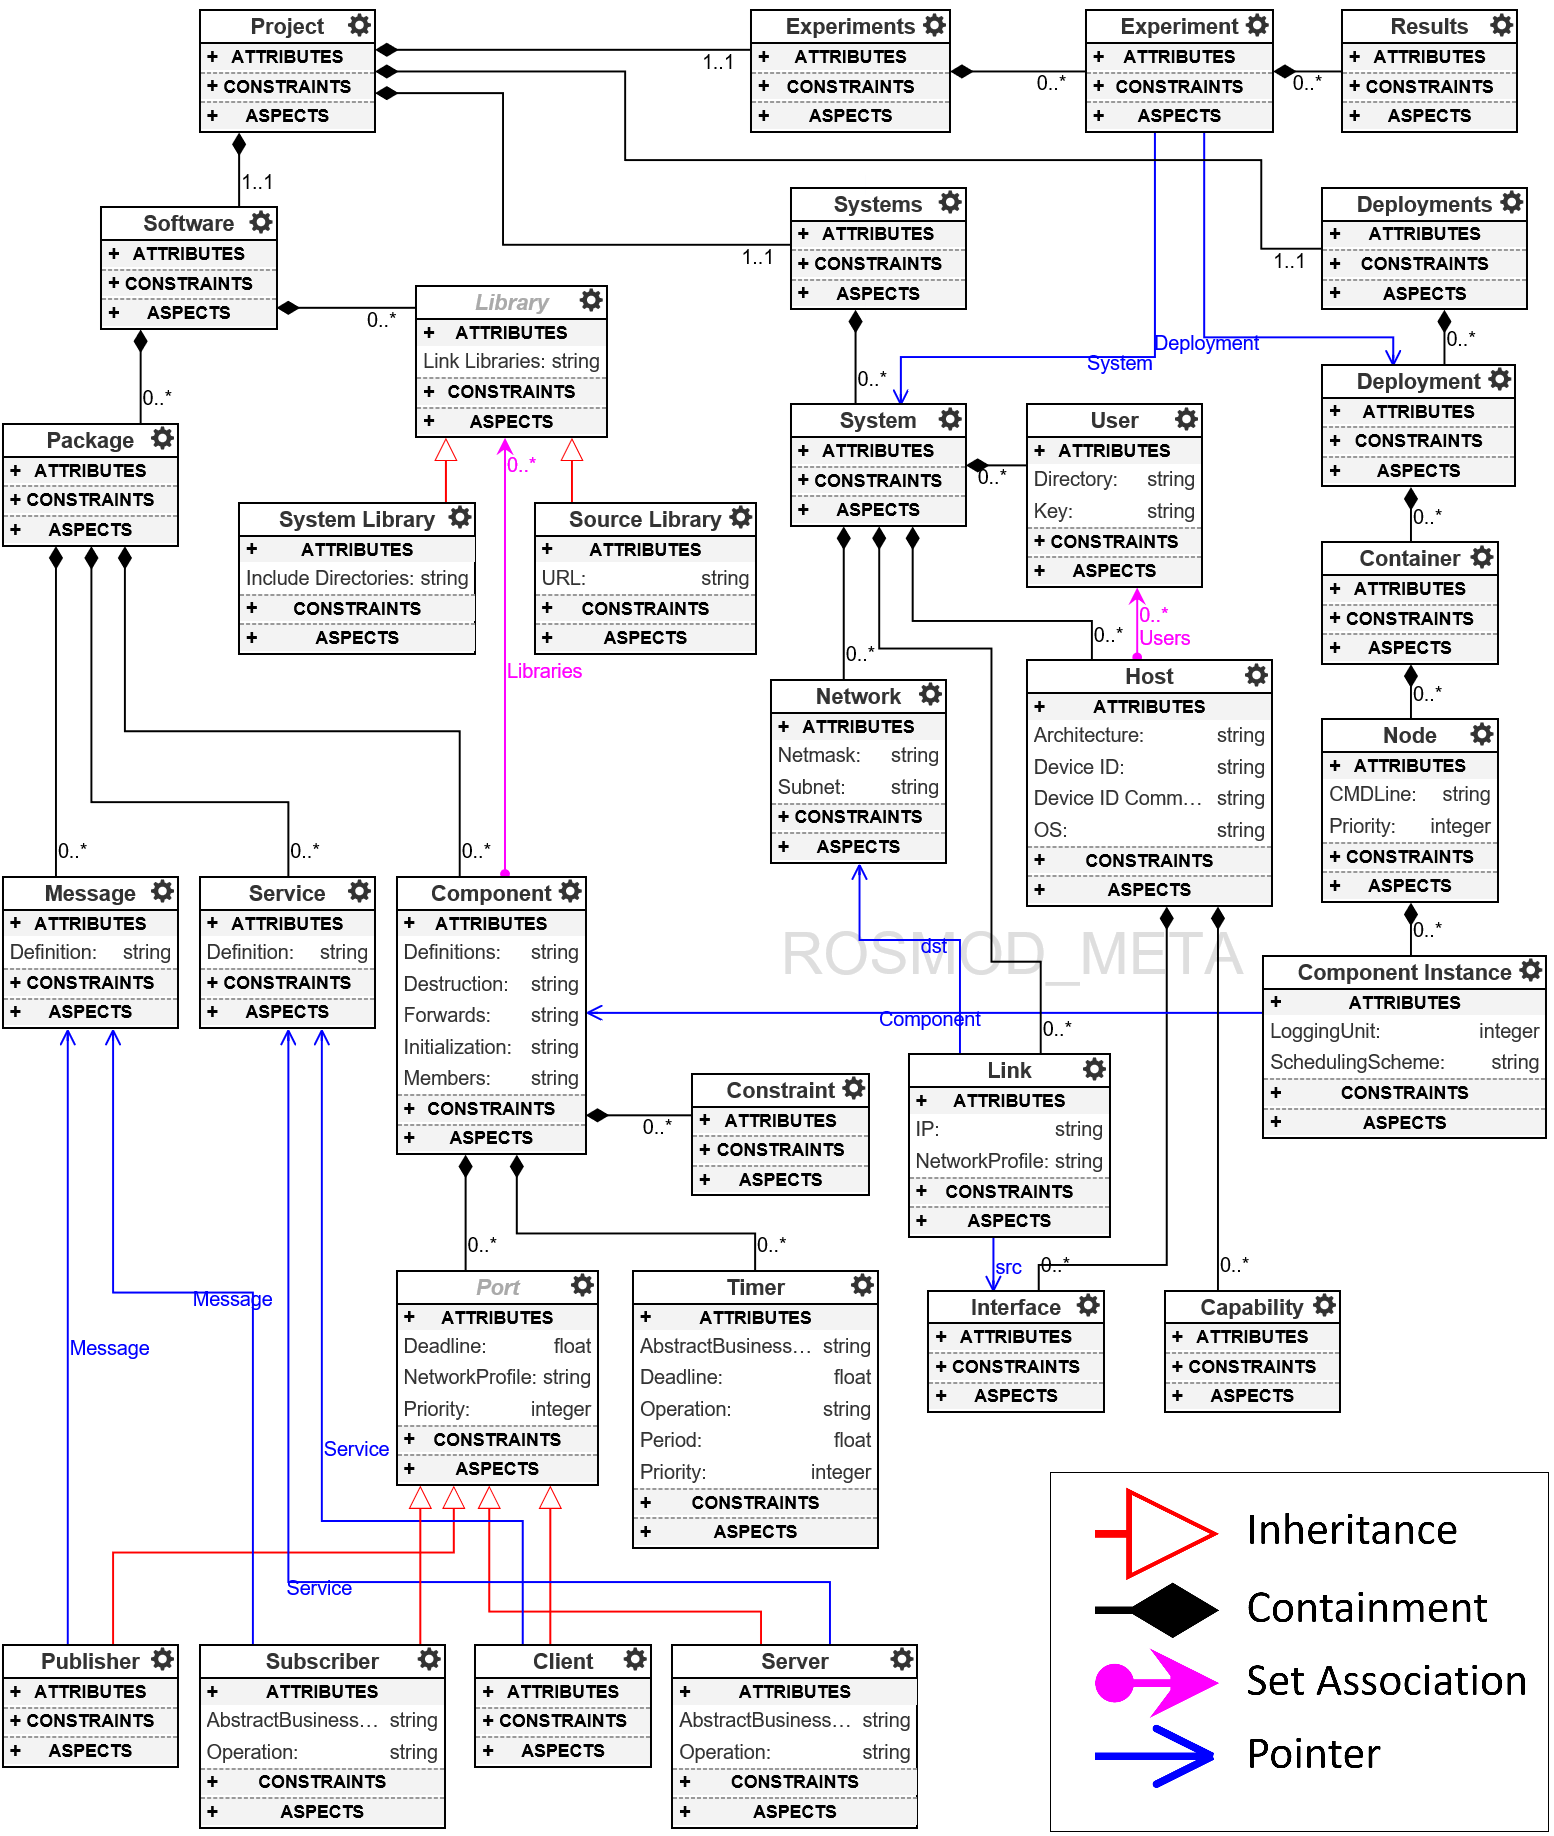
\includegraphics[width=\textwidth]{ROSMOD-Meta2.png}
	\caption{ROSMOD Metamodel.  Containment is specified from \emph{src} to \emph{dst} where the source has a containment attribute \emph{quantity}, meaning that \emph{quantity} objects of type \emph{src} can be contained in an object of type \emph{dst}. Pointers are specified as a one to one mapping from source to destination, using the name of the pointer. Sets allow for pointer containment. All objects contain a \emph{name} attribute of type \emph{string}, not shown for clarity.  Note: the metamodel is used to create the ROSMOD Modeling Language, but users do not see or interact with it; it is used to enforce proper model creation semantics.}
	\label{fig:ROSMOD_Project}	
\end{figure*}
\FloatBarrier

The top-level entity of RML is a \emph{Project}, which is shown in the upper left of Figure \ref{fig:ROSMOD_Project}.  The language supports a variety of modeling concepts that address structural and behavioral aspects for distributed embedded platforms. ROSMOD users can create models of software workspaces, required software libraries, embedded devices, network topologies, component constraints and hardware capabilities. The language also supports code development, particularly with regards to port interface implementations i.e. the execution code for operations owned and triggered by communication
ports or local timers. Below, we describe in detail the various aspects of this metamodel and how these concepts are integral to developing distributed CPS and rapid prototyping needs.

\subsubsection{Motivation for ROSMOD Software Model}

The goal of the ROSMOD software model is to provide a language to precisely model the application software. When using a DREMS-style component model, the software is primarily a collection of components, where each component is defined by its ports and timers. Building a precise model of the software has various benefits. Firstly, applying model-driven development techniques enables reuse of previously defined components i.e. a single component can be instantiated or copied or modified as required and executed on the runtime system. Secondly, the development time of the application can be reduced significantly as a large part of the runtime code can be fully generated based on templates. Lastly, a clear model of the software provides a canvas for design-time analysis. If the structural aspects of the software are captured in the model of the component assembly, and the behavioral properties of the components are encoded in the attributes of its ports and timers, then using translation rules, a design-time analysis model can be fully generated. 

\subsubsection{Software Model}

The \emph{Software} class in Figure \ref{fig:ROSMOD_Project} models a software workspace. A workspace, following ROS terminology, is a collection of applications that are developed and compiled together into binaries. Thus, each Software class can contain ROS applications, called \emph{Packages}, and \emph{Libraries} required for the applications. Packages consist of \emph{Messages}, \emph{Services} and \emph{Components}. Components contain a set of pointers to Libraries to establish dependence e.g. an \emph{ImageProcessor} component \emph{requires} OpenCV, an open-source computer vision library. Libraries are of two types: Source libraries and System libraries. Source libraries are standalone archives that can be retrieved, extracted and integrated into the software build system with no additional changes. System libraries are assumptions made by a software developer regarding the libraries pre-installed in the system. Here, system refers to the embedded device on which the component is intended to execute.

\emph{Messages} represent ROS message types used by publisher and subscriber ports for topic-based communication. Similarly, \emph{Services} describe the ROS peer-to-peer request-reply interaction pattern. Each service is characterized by a pair of messages, \emph{request} and \emph{response}. A client entity can call a service by sending a request message and awaiting a response. This interaction is presented to the user as a remote procedure call. Each ROSMOD component contains a finite set of communication ports. These ports refer to messages and services to concretize the communication interface. Components can also contain \emph{Timers} for time-triggered operation e.g. periodically sampling inertial measurement sensors while operating an unmanned aerial vehicle
(UAV).

\subsubsection{Motivation for ROSMOD System Model}

The goal of the ROSMOD system model is to provide a language to precisely model the network of computers capable of executing applications defined in the software model. The system model is necessary for both compilation and deployment. The software defined in the software model, and therefore the generated source code must be compiled down to a binary for runtime execution. An accurate model of the available runtime system provides necessary information for cross-compilation requirements and any integrated runtime load balancing features. The deployment framework can use the system model to find a suitable candidate device onto which the application processes are deployed. To automate this process, the system model must capture fine-grained details about each available device, including information such as the IP address, the user permissions, and means to access the device e.g. Secure Shell Protocol (SSH) \cite{ylonen2006secure}. As with the software model, this system model can be reused in all ROSMOD projects for a given hardware assembly, such as the RCPS tested. 

\subsubsection{System Model} 

A \emph{System Model} completely describes the hardware architecture of a system onto which the software can be deployed. A ROSMOD Project contains one or more \emph{Systems}. Each System contains one or more \emph{Hosts}, one or more \emph{Users}, one or more \emph{Networks}, and one or more \emph{Links}.  A host can contain one or more \emph{Network Interfaces}, which connect through a link to a network.  On this link the host's interface is assigned an IP address, which matches the subnet and netmask specification of the network. Additionally, a host has a set of references to users, which define the user-name, home directory, and ssh-key location for that user. The host itself has attributes which determine what kind of processor architecture it has, e.g. \emph{armv7l}, what operating system it is running, and lastly a combination of Device ID and Device ID Command which provide an additional means for specifying the type of host (and a way to determine it), for instance specifying the difference between a BeagleBone Black and an NVIDIA Jetson TK1 which both have armv7l architecture but can be separated by looking at the model name in the device tree.  Finally, a host may contain zero or more \emph{Capabilities} to which the component constraints (described in the previous section) are mapped.  The final relevant attribute is the \emph{Network Profile} attribute of a link. Using the network profile, which is specified as a time-series of bandwidth and latency values, we can configure the links of the network using the Linux TC to enforce time-varying bandwidth and latency. This network configuration is useful when running experiments on laboratory hardware for which the network is not representative of the deployed system's
network.

\subsection{Deployment Infrastructure}
\label{sec:Deployment_Infrastructure}

The workflow for software deployment is as shown Figure \ref{fig:workflow}. After the user has generated and compiled the software model into binary executables, they can run an experiment that has valid deployment model and system model references. Every ROSMOD workspace is generated with an additional \emph{node} package. This builds a generic node executable that can dynamically load libraries. When the software infrastructure generates and compiles the source code for the software model, the components are compiled into dynamically loadable libraries, one for each component definition along with a single executable corresponding to the generic node package. The first step the deployment infrastructure performs when running an experiment is generating the XML files which contain metadata about each ROS node modeled in the ROSMOD Deployment Model. This metadata includes the component instances in each node and the appropriate component libraries to be loaded. Based on the XML file supplied to the node executable, the node will behave as one of the ROS nodes in the deployment model. This allows for a reusable framework where a generic executable (1) loads an XML file, (2) identifies the component instances in the node, (3) finds the necessary component libraries to load and (4) spawns the executor threads bound to each component.

\begin{figure}[ht]
	\centering
	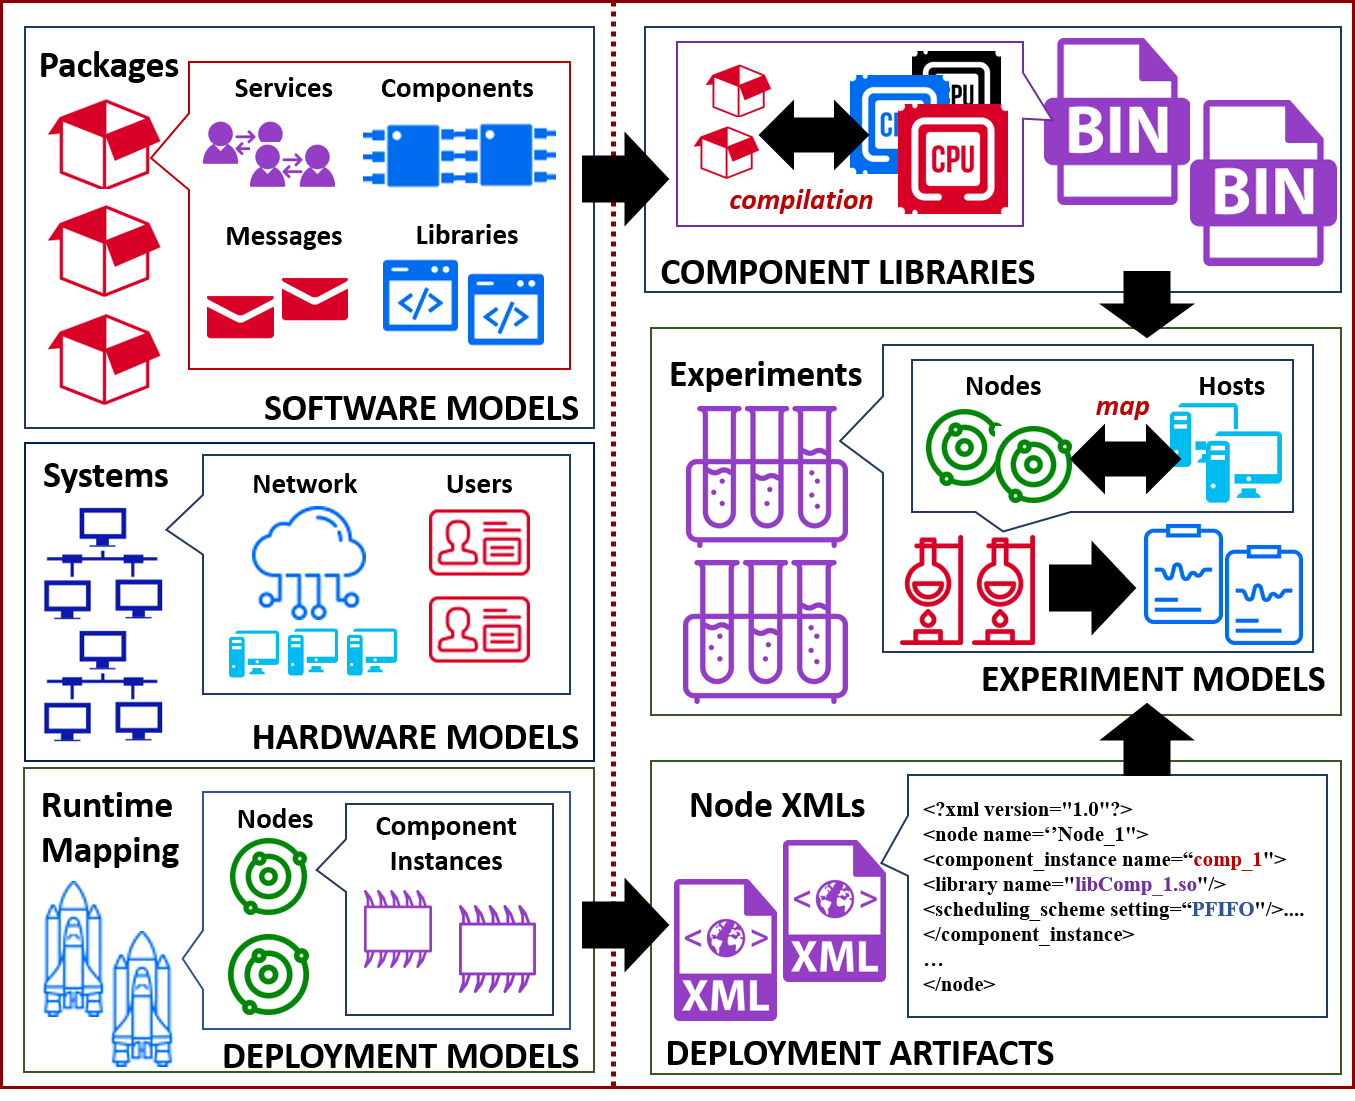
\includegraphics[width=\textwidth]{DeploymentInfrastructure.png}
	\caption{Software Deployment Workflow}
	\label{fig:workflow}
\end{figure}
\FloatBarrier

\section{Evaluation of Timing Analysis Results}

Experimental validation should demonstrate that online measurements of the real-time system match with the timing analysis results in a way that the timing analysis results are always close but conservative. The goal of the analysis is to obtain a fairly accurate estimation of the runtime behavior i.e. estimates of component timing behavior that isn't so conservative that the results are useless. If the real execution of a specific operation takes 100 milliseconds and the timing analysis is 135 milliseconds, then this is close but conservative. On the other hand, if the design-time analysis predicts the execution time to be in the order of seconds or tens of seconds, then the analysis is conservative but grossly over-estimate. One of the biggest assumptions in our CPN work is the knowledge of worst-case execution times of the individual steps in the component operations. We have previously designed \cite{SEUS} a business-logic modeling grammar that captures the temporal behavior of component operations, especially WCET metrics for the different code blocks inside an operation. For example, consider a simple client-server example as shown in Figure \ref{fig:rmi_application}. The client component is periodically triggered by an internal timer and executes a synchronous remote method invocation to a remote server component. The interaction here demands that the client component be blocked for the duration of time it takes the server to receive the operation, process its message queue, execute the relevant callback, and respond with output. 

Note that in Figure \ref{fig:rmi_application}, we only annotate isolated code blocks that take a fixed amount of execution time on a specific hardware architecture. These are the only measurements that we can reliably make with repeated testing and instrumentation. The client-side blocking delay is not measured because the number of factors responsible for this delay are numerous e.g. server's message queue state, scheduling non-determinism, network delays etc. In order to be able to predict this delay, we need to use state space analysis and search through the tree of possible executions to identify the worst-case blocking delay. This also means that our CPN model must capture and account for such delay-causing factors. 

The remainder of this section presents various primitive interaction patterns and assemblies that have been evaluated. The results are restricted to simple cases, though we have tested on medium-to-large scale examples spanning 25-30 computing nodes, and with up to a 100 components. The scalability of our model, however, is not within the scope of this paper as we have previously evaluated this metric \cite{SEUS}. As mentioned earlier, in all of our tests, we use the ROS \cite{ROS} middleware and our ROSMOD \cite{kumarROSMOD} component model. 

\subsection{Understanding the CPN Analysis Plots}

By performing state space analysis, we are analyzing a bounded tree of possible component behaviors. By identifying the worst-case execution trace in this tree, we're able to obtain a suitable conservative candidate execution that represents a possible behavior. Once this trace is identified, we plot the response time behavior of all components in this trace. This pattern is followed in all of the following plots. Figure \ref{fig:understanding-the-plots} describes the analysis plots presented later in this chapter. Each subplot in this figure represents the execution of a component operation. The x axis of this plot represents the analysis time, and the y axis represents the response time of the operation. Each execution is shown as a rectangular pulse, the amplitude of which is the worst-case response time (WCRT) of the operation i.e. the time taken for the operation to complete (response) from when the executor thread was released for execution (trigger). The rising edge of the pulse represents the enqueue time stamp of the operation i.e. the time instant when a request for this operation was enqueued onto the component message queue. The falling edge of the pulse represents the completion time stamp i.e. the time instant when the component executor thread has completed execution of the operation and is ready to service the next request waiting in the queue. Since the response time of the operation is calculated from the enqueue time instant, the plot can have intersecting pulses, as shown in the second subplot. Here a new operation request is enqueued onto the message queue while an existing instance of the operation request is being executed by the component executor thread. 

\begin{figure}[h]
	\centering
	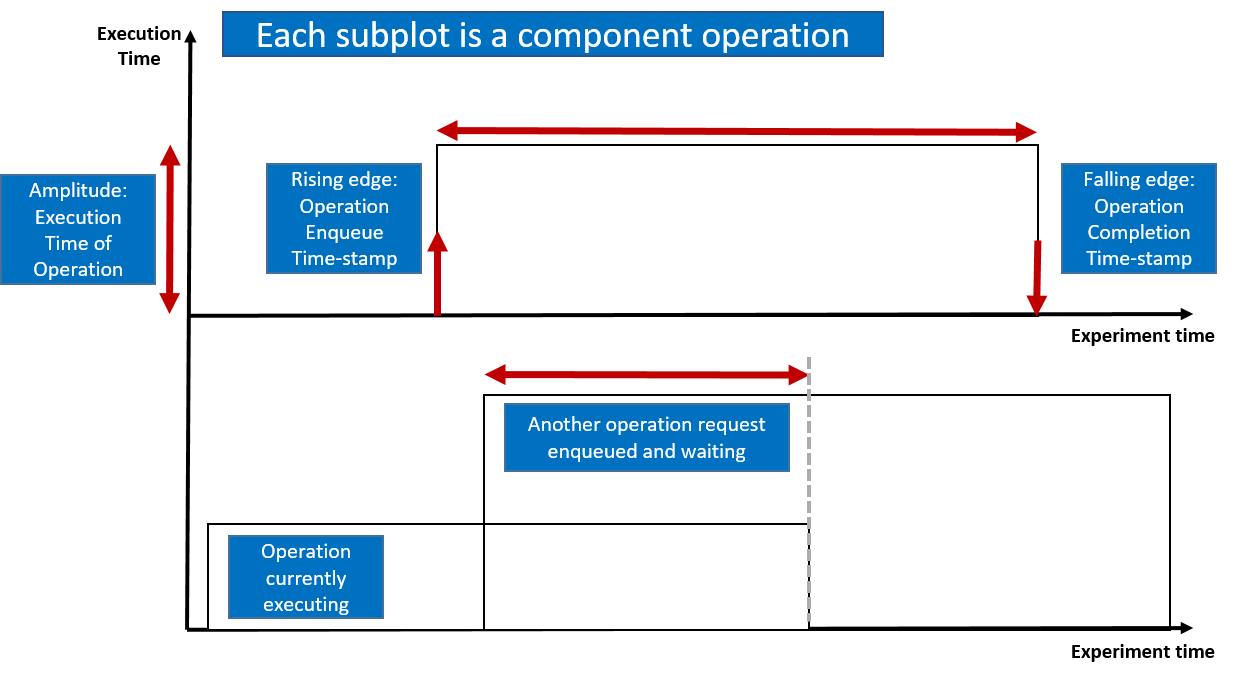
\includegraphics[width=\textwidth]{understanding-the-plots}
	\caption{Interpreting Execution Time Plots}
	\label{fig:understanding-the-plots}
\end{figure}
\FloatBarrier


\subsection{Client-Server Interactions}

As shown in Figure \ref{fig:rmi_application}, a simple client server example involves a periodically triggered client component that fetches data from a remote server. Figure \ref{fig:client-server} shows our experimental trace of a simple distributed client-server sample. The client (client\_timer\_operation) is triggered every 500 ms, and performs floating-point calculations in a loop requiring the services of a remote operation.  %The loop bound is a random variable having a uniform distribution between some peak iteration count and 60\% of this peak. 
The server (Power\_operation) periodically receives this operation request and responds to it, taking about 1.2s to complete each operation instance. In this experiment, these component threads are running at high uninterrupted real-time priorities. 

\begin{figure}[h]
	\centering
	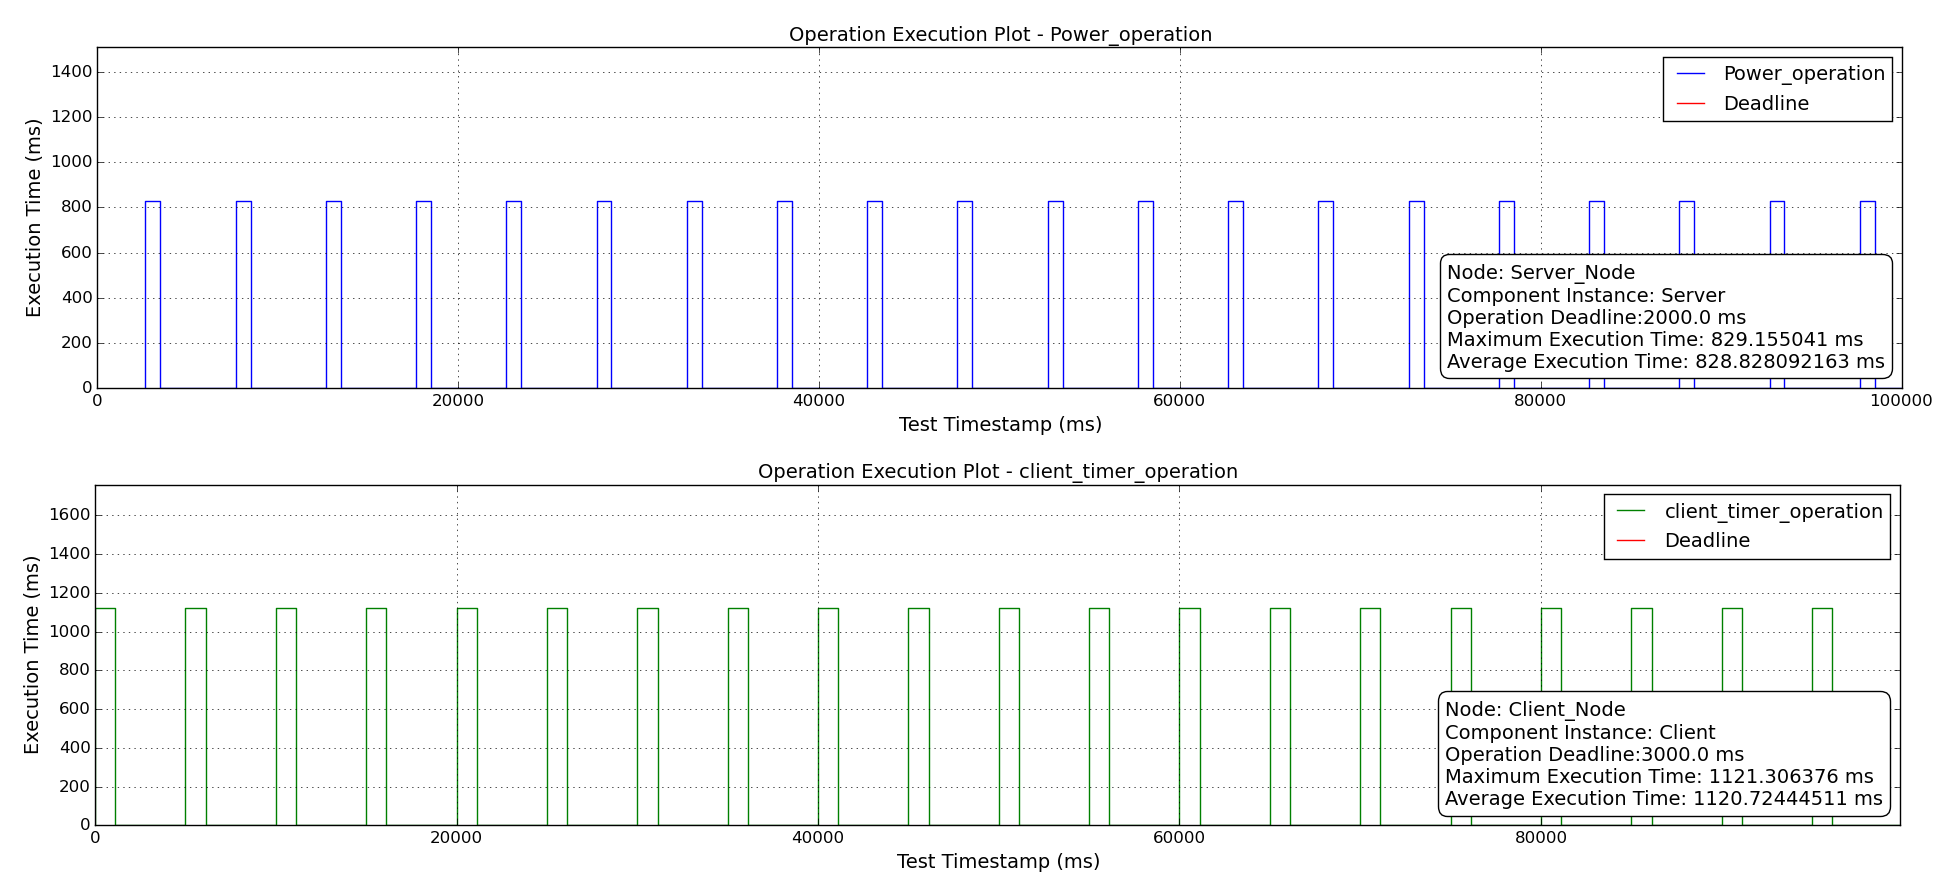
\includegraphics[width=\textwidth]{client-server}
	\caption{Experimental Observation: Client-Server Interactions}
	\label{fig:client-server}
\end{figure}
\FloatBarrier

Figure \ref{fig:client-server-cpn} shows the execution time plot derived from our CPN. As expected, since there are no other interruptions on the server side, the server is able to promptly respond to the client.

\begin{figure}[h]
	\centering
	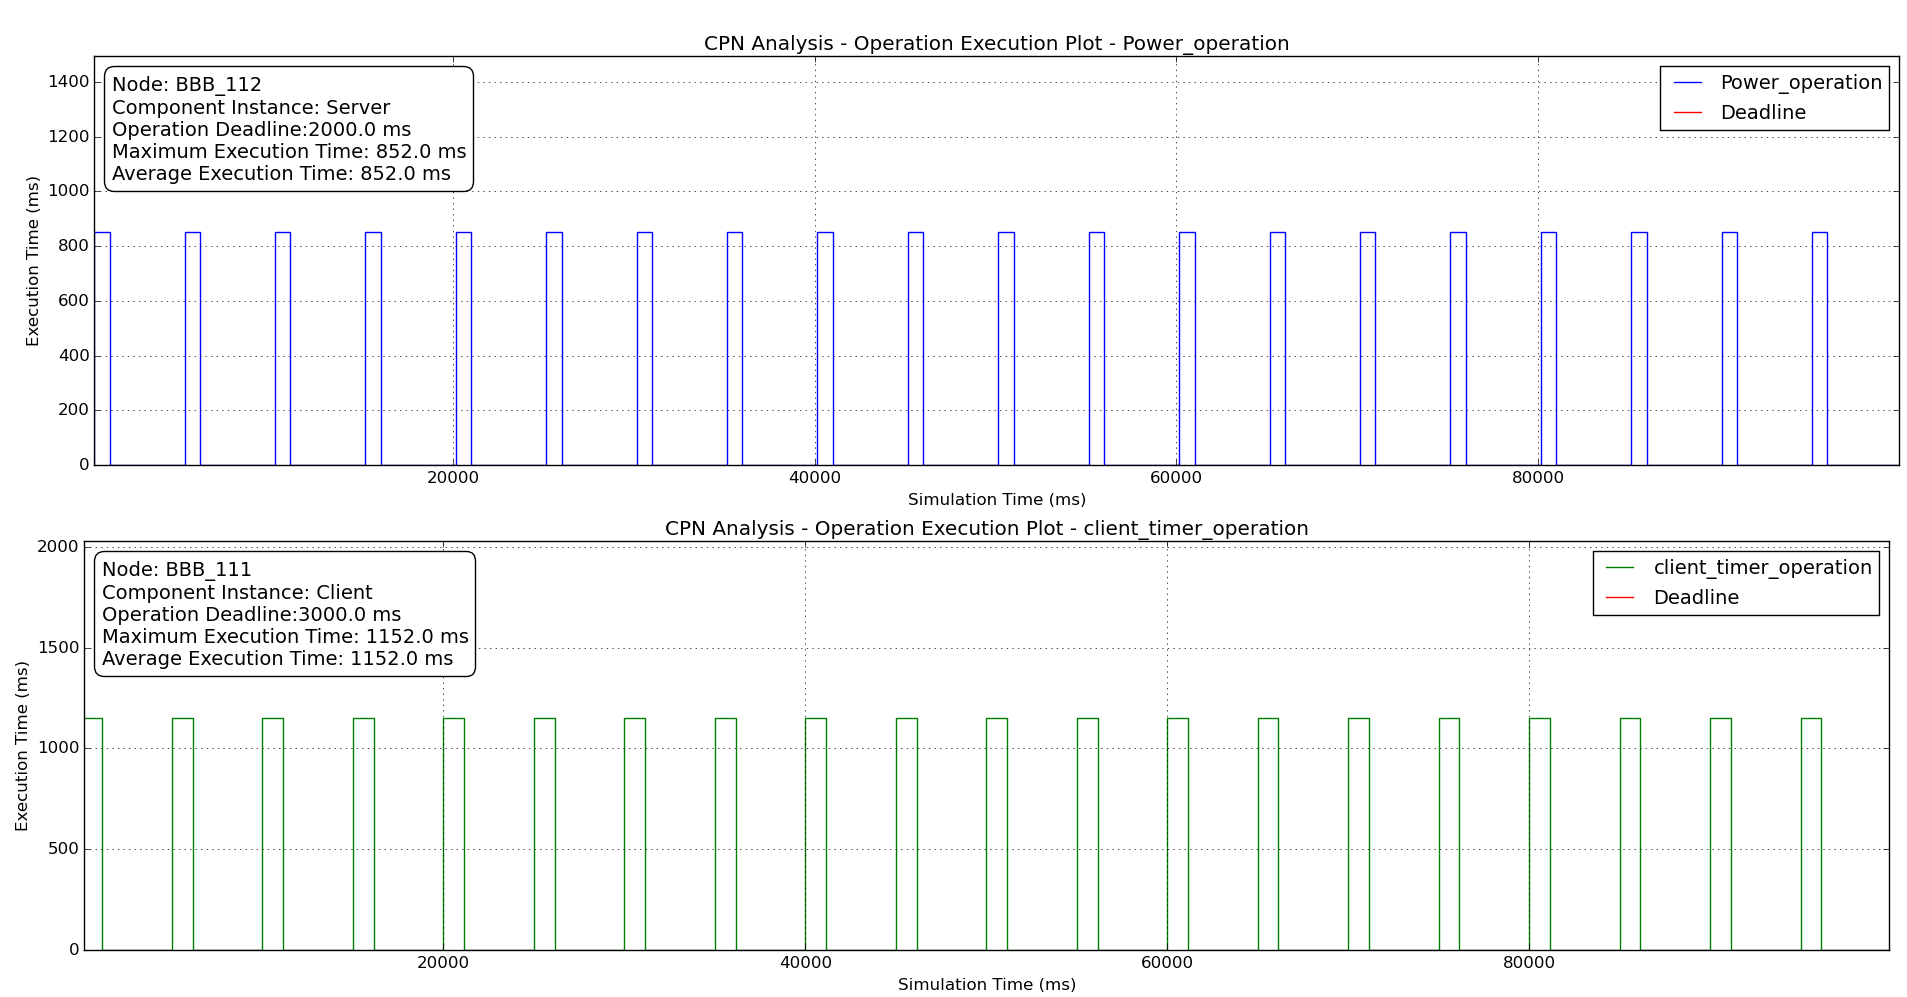
\includegraphics[width=\textwidth]{client-server-cpn}
	\caption{CPN Analysis Results: Client-Server Interactions}
	\label{fig:client-server-cpn}
\end{figure}
\FloatBarrier

Table \ref{tbl:client-server} shows a summary of these results. Similar tables are included as part of all other experiments in this section. 

\begin{table}[]
\centering
\caption{Client Server Example - Summary of Results}
\label{tbl:client-server}
\begin{tabular}{|c|c|c|c|c|}
\hline
\textbf{\begin{tabular}[c]{@{}c@{}}Operation\\ Name\end{tabular}}  & \textbf{\begin{tabular}[c]{@{}c@{}}Component\\ Name\end{tabular}} & \textbf{\begin{tabular}[c]{@{}c@{}}Experimental \\ WCRT (ms)\end{tabular}} & \textbf{\begin{tabular}[c]{@{}c@{}}Timing Analysis\\ WCRT (ms)\end{tabular}} & \textbf{\begin{tabular}[c]{@{}c@{}}Deadline\\ (ms)\end{tabular}} \\ \hline
\begin{tabular}[c]{@{}c@{}}Power\\ Operation\end{tabular}          & Server                                                            & 829.155041                                                                                  & 852.0                                                                                                & 2000                                                             \\ \hline
\begin{tabular}[c]{@{}c@{}}Client\\ Timer\\ Operation\end{tabular} & Client                                                            & 1121.306376                                                                                 & 1152.0                                                                                               & 3000                                                             \\ \hline
\end{tabular}
\end{table}

\subsubsection{Bad Designs}

The goal of our CPN timing analysis is to identify bad component designs, unacceptable execution times, response times etc. There are various ways in which we can accidentally design a poorly performing client-server interaction. In the above case, the server operation takes 852 ms in its worst-case before responding to the client and unblocking the client executor thread. If instead, the server operation took 8.5 seconds, the client component will stay blocked for 10 times longer and the client timer expiries will not be serviced faster than the timer periods. This shows a simple use-case where the currently blocked client timer operation is starving subsequent timer expiries from being handled promptly. Figure \ref{fig:client-server-bad-case} shows our CPN predictions after simply changing this server execution time. 

\begin{figure}[h]
	\centering
	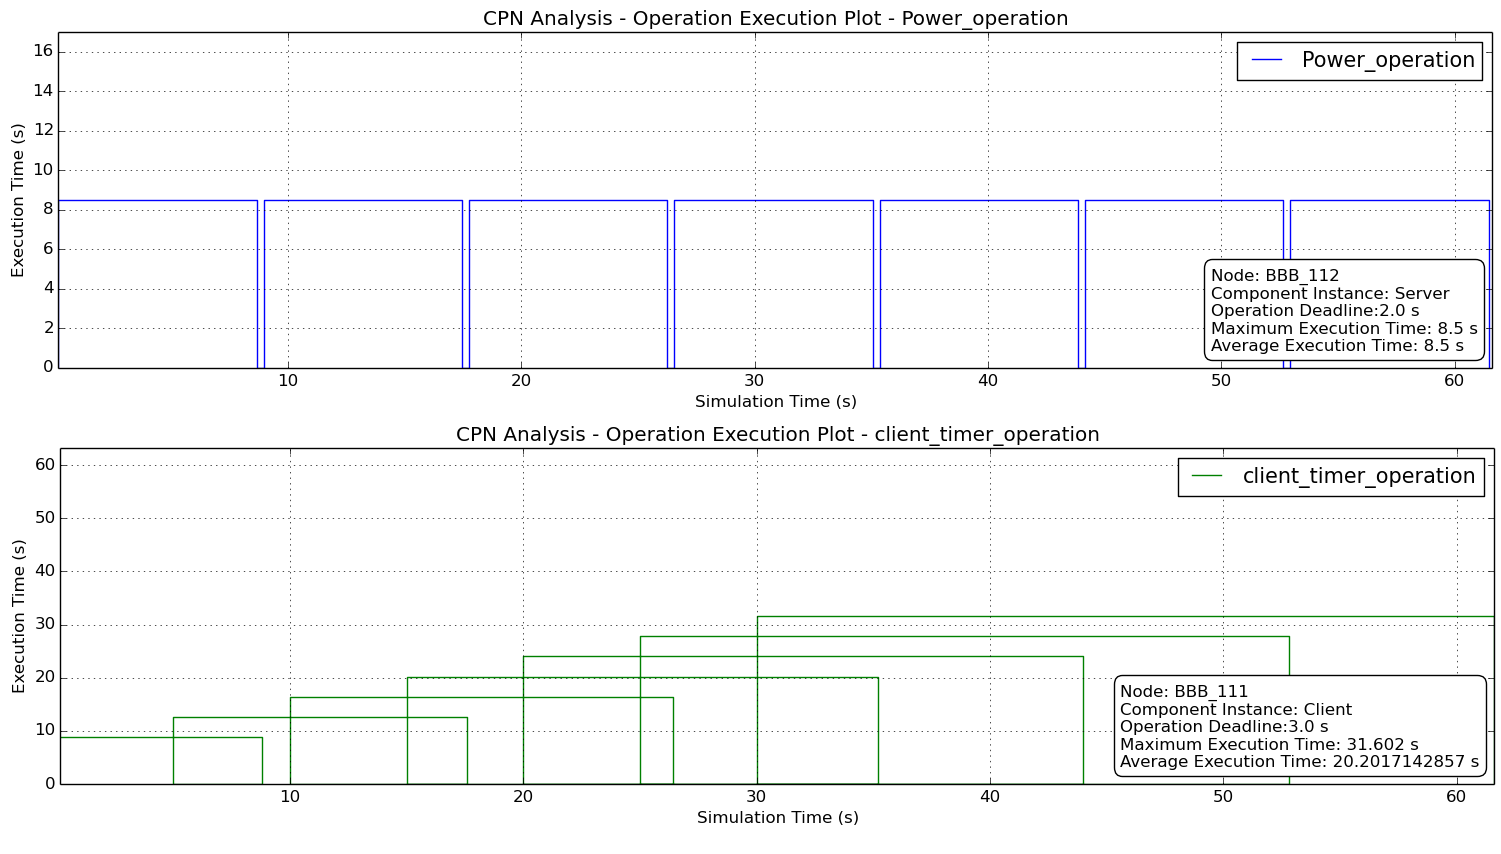
\includegraphics[width=\textwidth]{client-server-bad-case}
	\caption{CPN Analysis Results: Client-Server Response Times in Bad Designs}
	\label{fig:client-server-bad-case}
\end{figure}
\FloatBarrier

The execution time of the each new client-side timer operation is worse than the previous since the operation is spending much longer waiting in the queue. Recall that the execution time of a component operation includes the waiting time in the message queue. Even with a bounded state space that spans just 1 minute, it is clear that the client component message queue size is monotonically increasing. This is a use case where a client component execution is affected by delays caused on a remote server. Each client-server interaction delay will only be worsened when the server component has other operations to tend to aside from the client requests. 

\subsection{Publish-Subscribe Interactions}

Similar to the earlier example, consider the ROSMOD publish-subscribe interaction. A publisher is periodically triggered by a timer when this component broadcasts a message on a topic. A subscribing component receives this message and performs some computation. In this case, the timer period is set to 2 seconds i.e. every 2 seconds, these two component interact via publish-subscribe messaging passing. 

\begin{figure}[h]
	\centering
	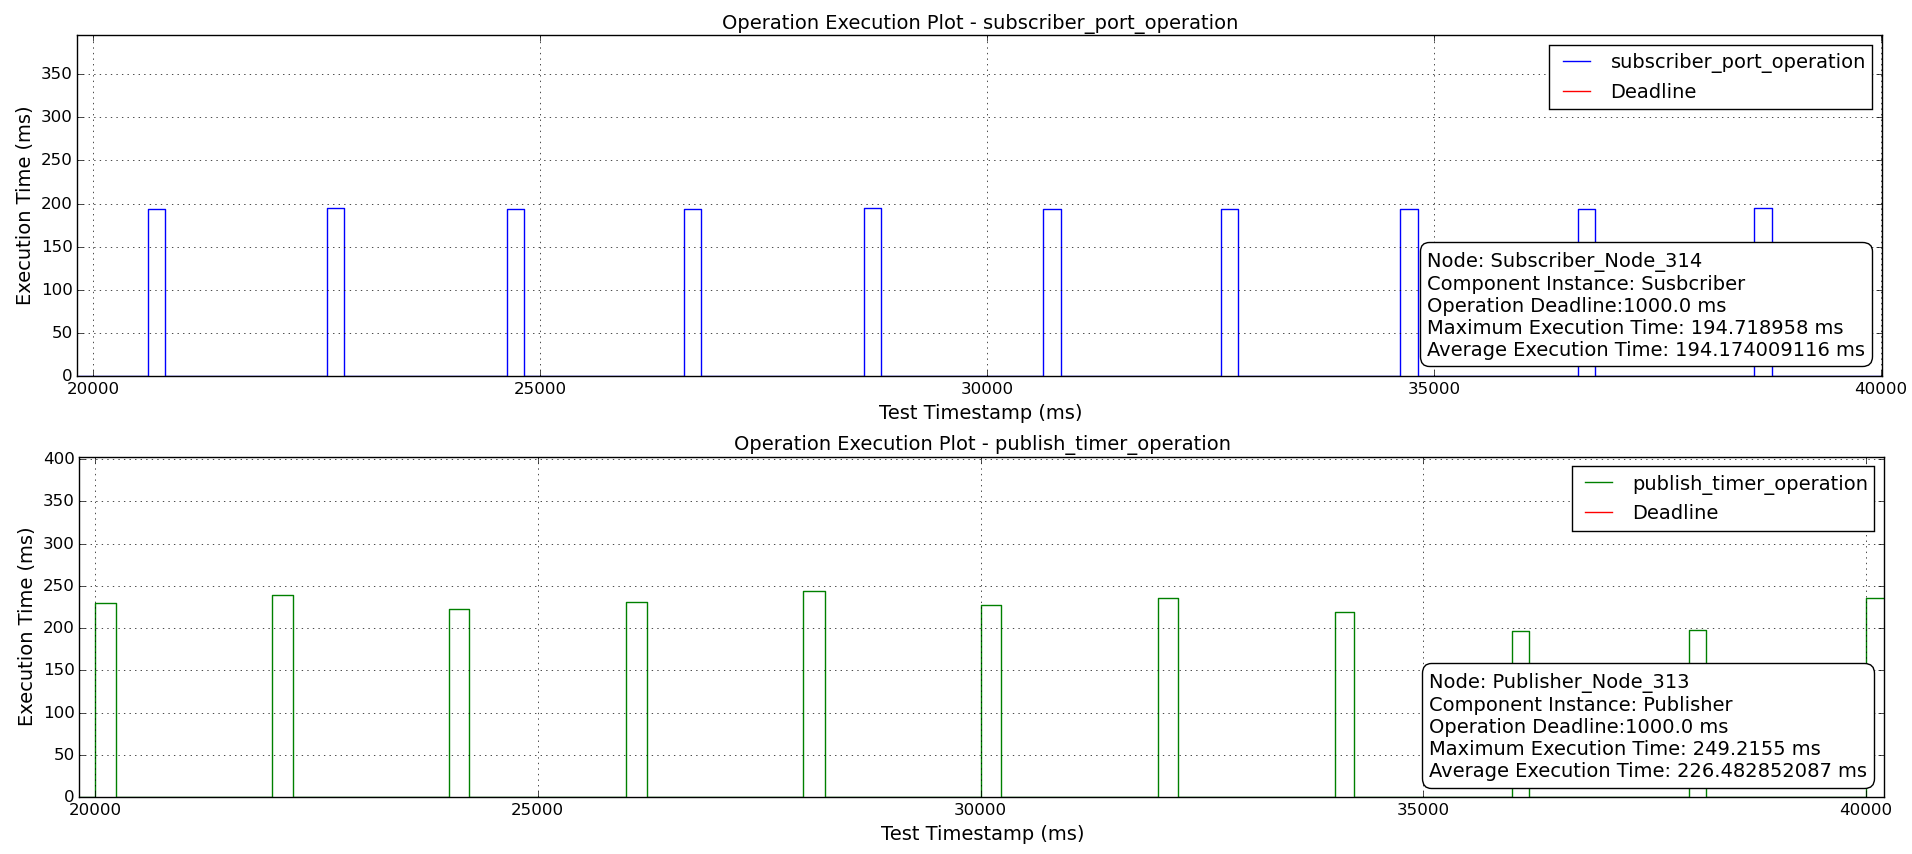
\includegraphics[width=\textwidth]{publish-subscribe}
	\caption{Experimental Observation: Publish-Subscribe Interactions}
	\label{fig:publish-subscribe}
\end{figure}
\FloatBarrier

Figure \ref{fig:publish-subscribe} shows our testbed observations and Figure \ref{fig:publish-subscribe-cpn} shows our CPN analysis results. As evident, the CPN results closely match and validate this sample. Table \ref{tbl:publish_subscribe} summarizes the results.

\begin{figure}[h]
	\centering
	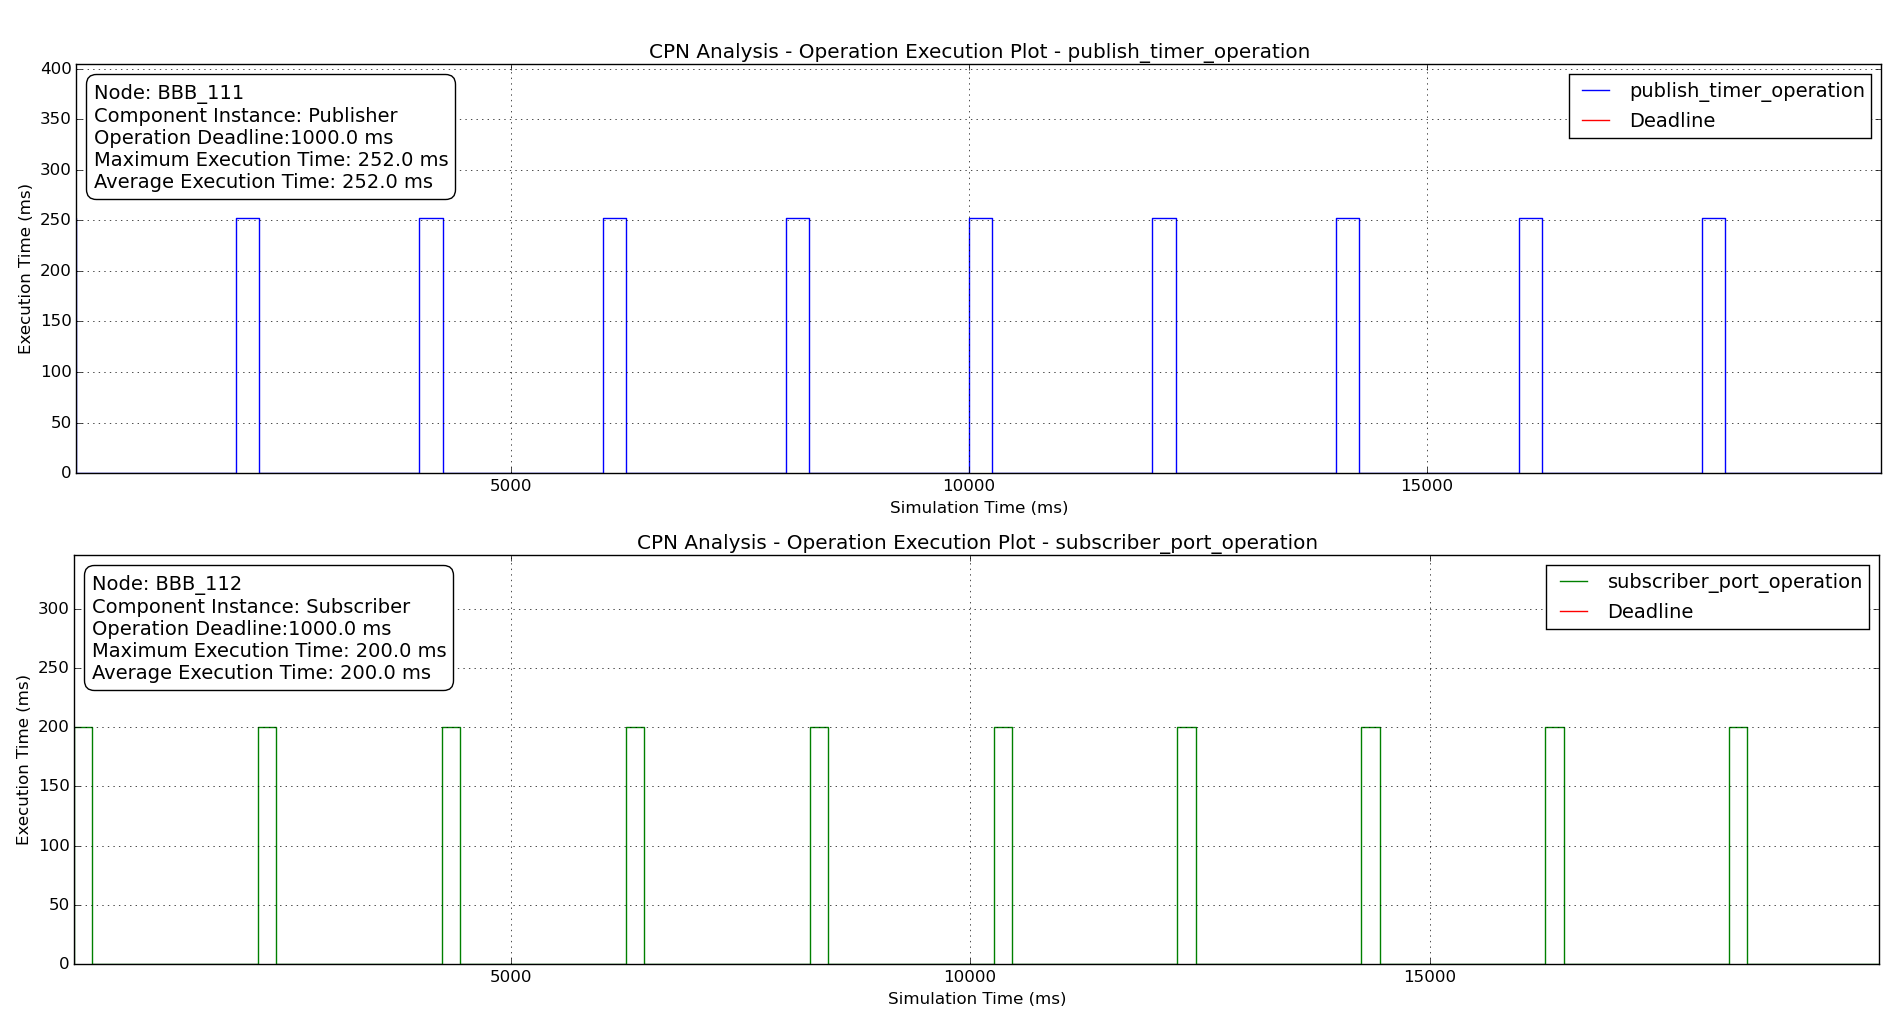
\includegraphics[width=\textwidth]{publish-subscribe-cpn}
	\caption{CPN Analysis Results: Publish-Subscribe Interactions}
	\label{fig:publish-subscribe-cpn}
\end{figure}
\FloatBarrier

\begin{table}[]
\centering
\caption{Publish Subscribe Example -- Summary of Results}
\label{tbl:publish_subscribe}
\begin{tabular}{|c|c|c|c|c|}
\hline
\textbf{\begin{tabular}[c]{@{}c@{}}Operation\\ Name\end{tabular}} & \textbf{\begin{tabular}[c]{@{}c@{}}Component\\ Name\end{tabular}} & \textbf{\begin{tabular}[c]{@{}c@{}}Experimental\\ WCRT (ms)\end{tabular}} & \textbf{\begin{tabular}[c]{@{}c@{}}Timing Analysis\\ WCRT (ms)\end{tabular}} & \textbf{\begin{tabular}[c]{@{}c@{}}Deadline\\ (ms)\end{tabular}} \\ \hline
\begin{tabular}[c]{@{}c@{}}Subscriber\\ Port\\ Operation\end{tabular} & Subscriber & 194.718958 & 200.0 & 1000 \\ \hline
\begin{tabular}[c]{@{}c@{}}Publisher\\ Timer\\ Operation\end{tabular} & Publisher & 249.2155 & 252.0 & 1000 \\ \hline
\end{tabular}
\end{table}

\subsubsection{Bad Designs}

Similar to the client-server example, we can explore another accidental bad design that may become hard to track. In a publish-subscribe interaction, the publisher and the subscriber are completely detached from each other i.e. delays in the subscriber operation do not affect the publisher. So, the only way the publisher component can affect its own behavior is how it is triggered. Periodically triggered data dissemination is the most commonly used streaming pattern aside from event-driven messaging. Here, if the period of the timer is decreased from 2 s to 10 ms, the publisher gets triggered too frequently and is seriously affected by a local design flaw.  

\begin{figure}[h]
	\centering
	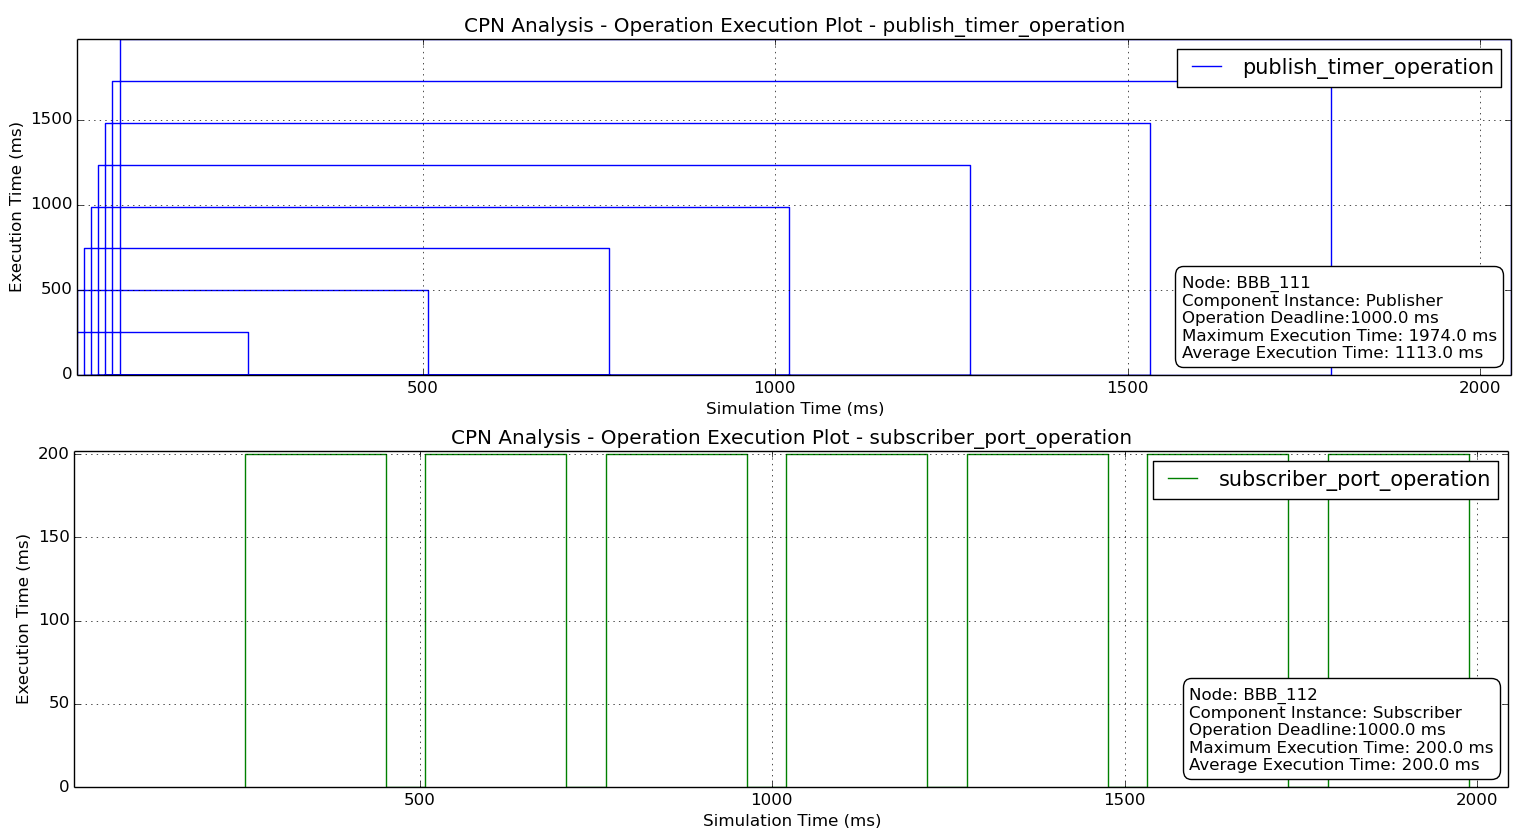
\includegraphics[width=\textwidth]{publish-subscribe-bad-case}
	\caption{CPN Analysis Results: Time-triggered Publisher -- Periodicity Issues}
	\label{fig:publish-subscribe-bad-case}
\end{figure}
\FloatBarrier

Figure \ref{fig:publish-subscribe-bad-case} shows the CPN results for this design. The subscriber still performs as expected taking 200 ms to process each incoming message. But the publishing component is affected by the periodicity of its trigger. The publish\_timer fires every 10 ms, and at each expiry enqueues a timer operation request onto the publisher component's message queue. Each timer operation itself takes about 250 ms i.e. 25 times of the periodicity of its trigger. The inevitable result of this design is the monotonically rising execution times of each subsequent timer operation due to progressively delayed response. Here, the $t\_response\_time$ = $t\_dequeue$ - $t\_enqueue$ becomes progressively worse and eventually the publisher's message queue overflows. In the real experiment, we were unable to access the publisher component's device via remote shell as the device CPU was saturated. 

\subsection{Trajectory Planner}

In the past \cite{kumar2014colored}, we have used a \emph{Trajectory Planner} deployment to illustrate the utility of our state space analysis. As shown in Figure \ref{fig:trajectory-planner-components}, a Sensor component is periodically triggered every second by the \emph{sensor\_timer} at which point it publishes a notification to the Trajectory Planner, alerting the planner of new sensor state. The planner component receives this notification on its \emph{state\_subscriber}. On receiving this message, the planner executes a remote method invocation to the \emph{compute} server located in the Sensor, blocked and waiting for a response. At this point, the \emph{compute\_operation} is executed on the Sensor which returns the updated sensor state. This unblocks the planner component which uses the new sensor state to perform trajectory planning tasks. 

\begin{figure}[h]
	\centering
	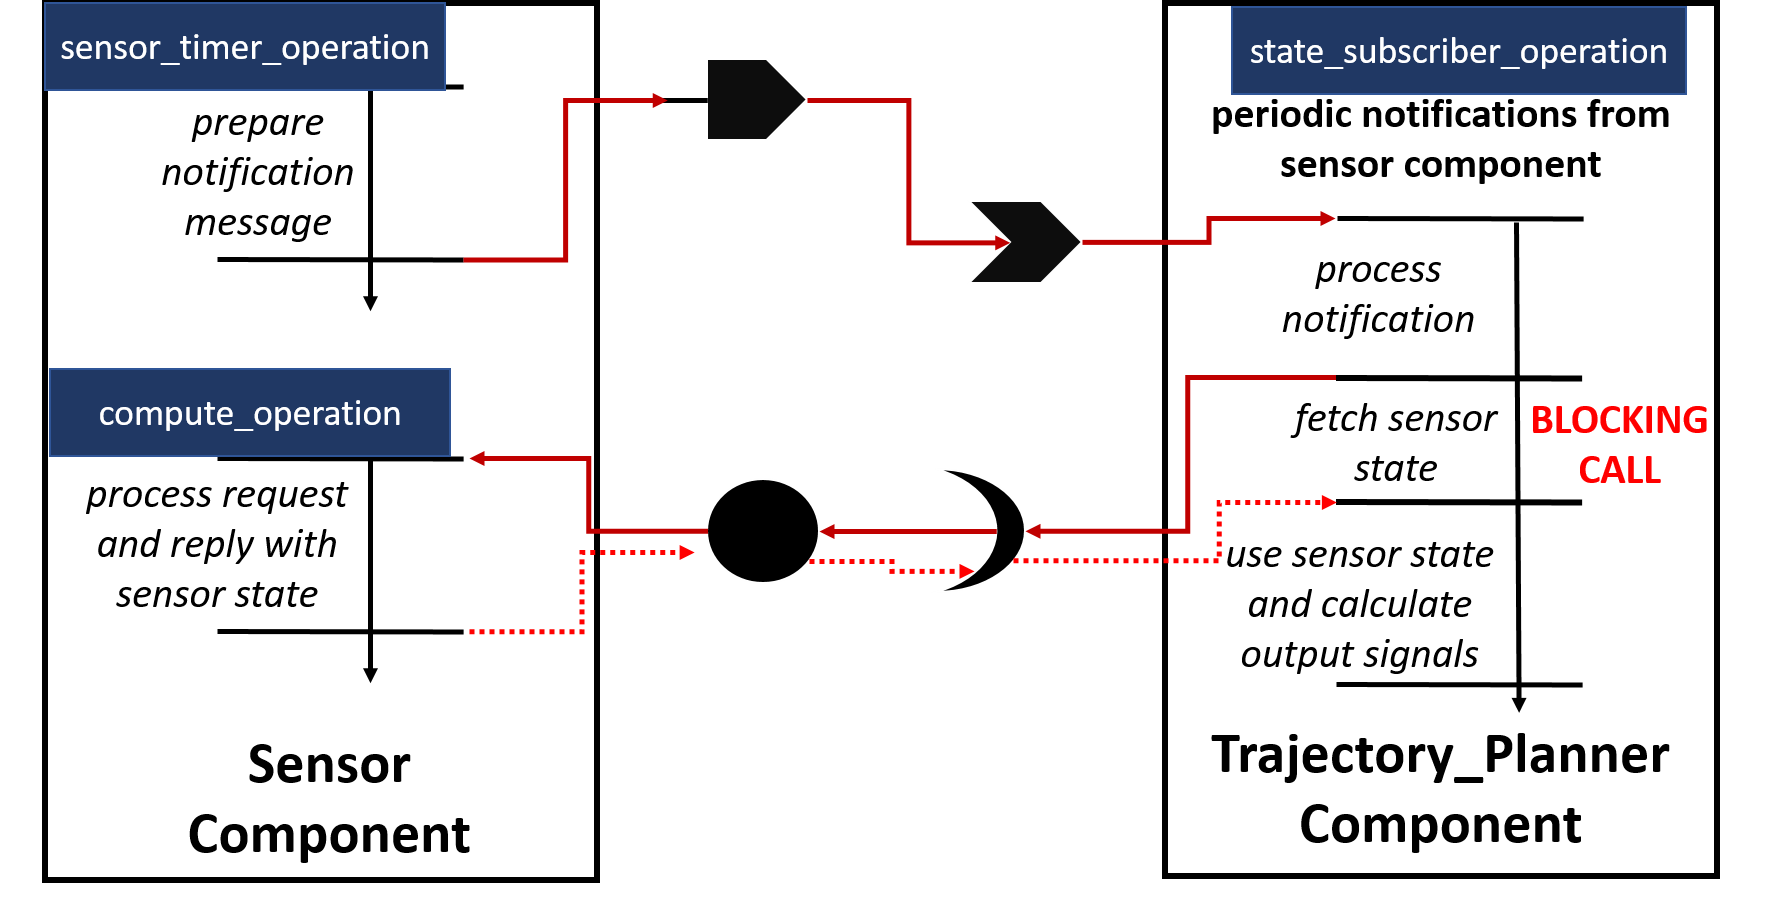
\includegraphics[width=\textwidth]{trajectory-planner-components}
	\caption{Trajectory Planner Test}
	\label{fig:trajectory-planner-components}
\end{figure}
\FloatBarrier

Figure \ref{fig:trajectory-planner} shows the execution time plot of this sample where the sensor updates happen once a second. Figure \ref{fig:trajectory-planner-cpn} presents the CPN analysis plot and Table \ref{tbl:trajectory-planner} summarizes the results.

\begin{figure}[h]
	\centering
	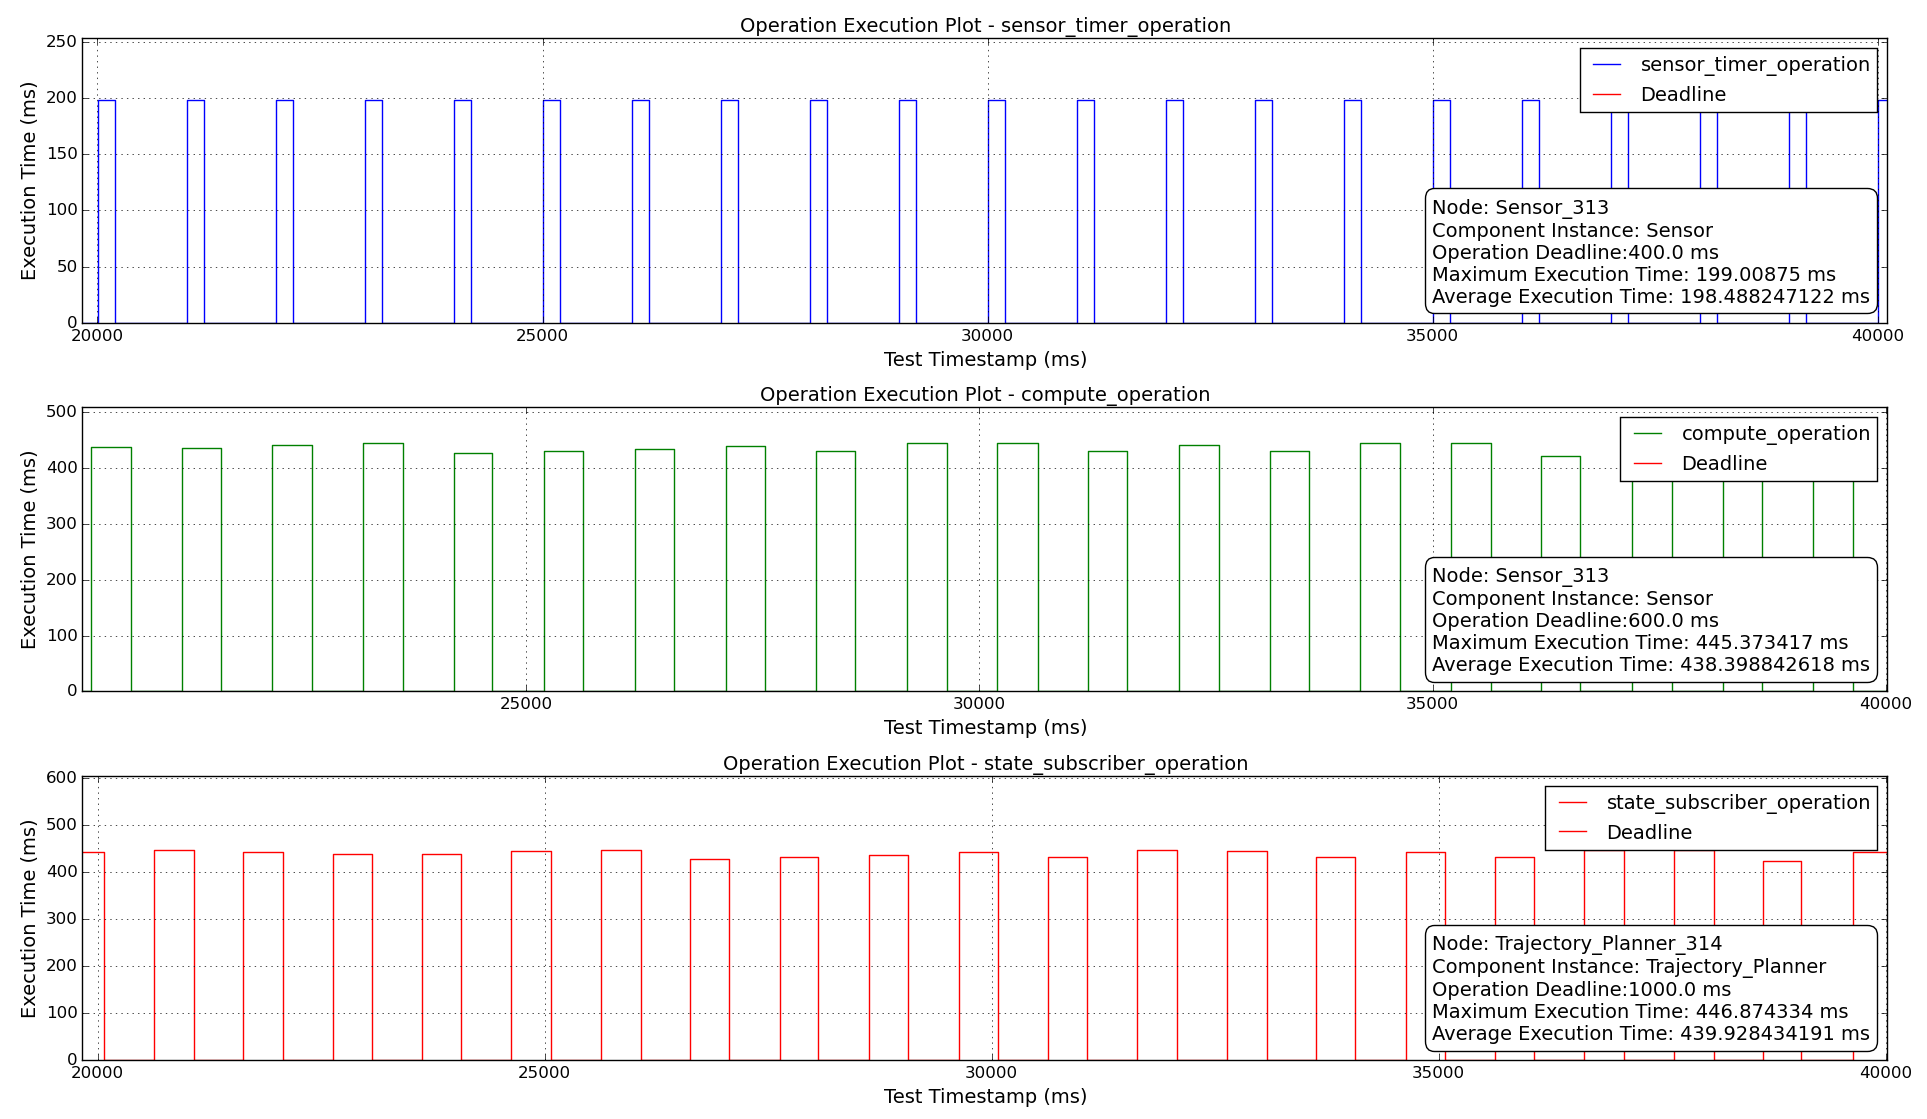
\includegraphics[width=\textwidth]{trajectory-planner}
	\caption{Experimental Observation: Trajectory Planner}
	\label{fig:trajectory-planner}
\end{figure}
\FloatBarrier

This is a common interaction pattern in Cyber-Physical systems since embedded sensors are updated at a much higher frequency than a path planning entity. Thus, the planner can query the sensor at a lower rate to sample the sensor state. In this example, the planner is matching the frequency of the sensor since the execution cost is low. However, when more components are added to this deployment, the planner would have to fetch sensor state less frequently so as to not affect other system-level deadlines. 

\begin{figure}[h]
	\centering
	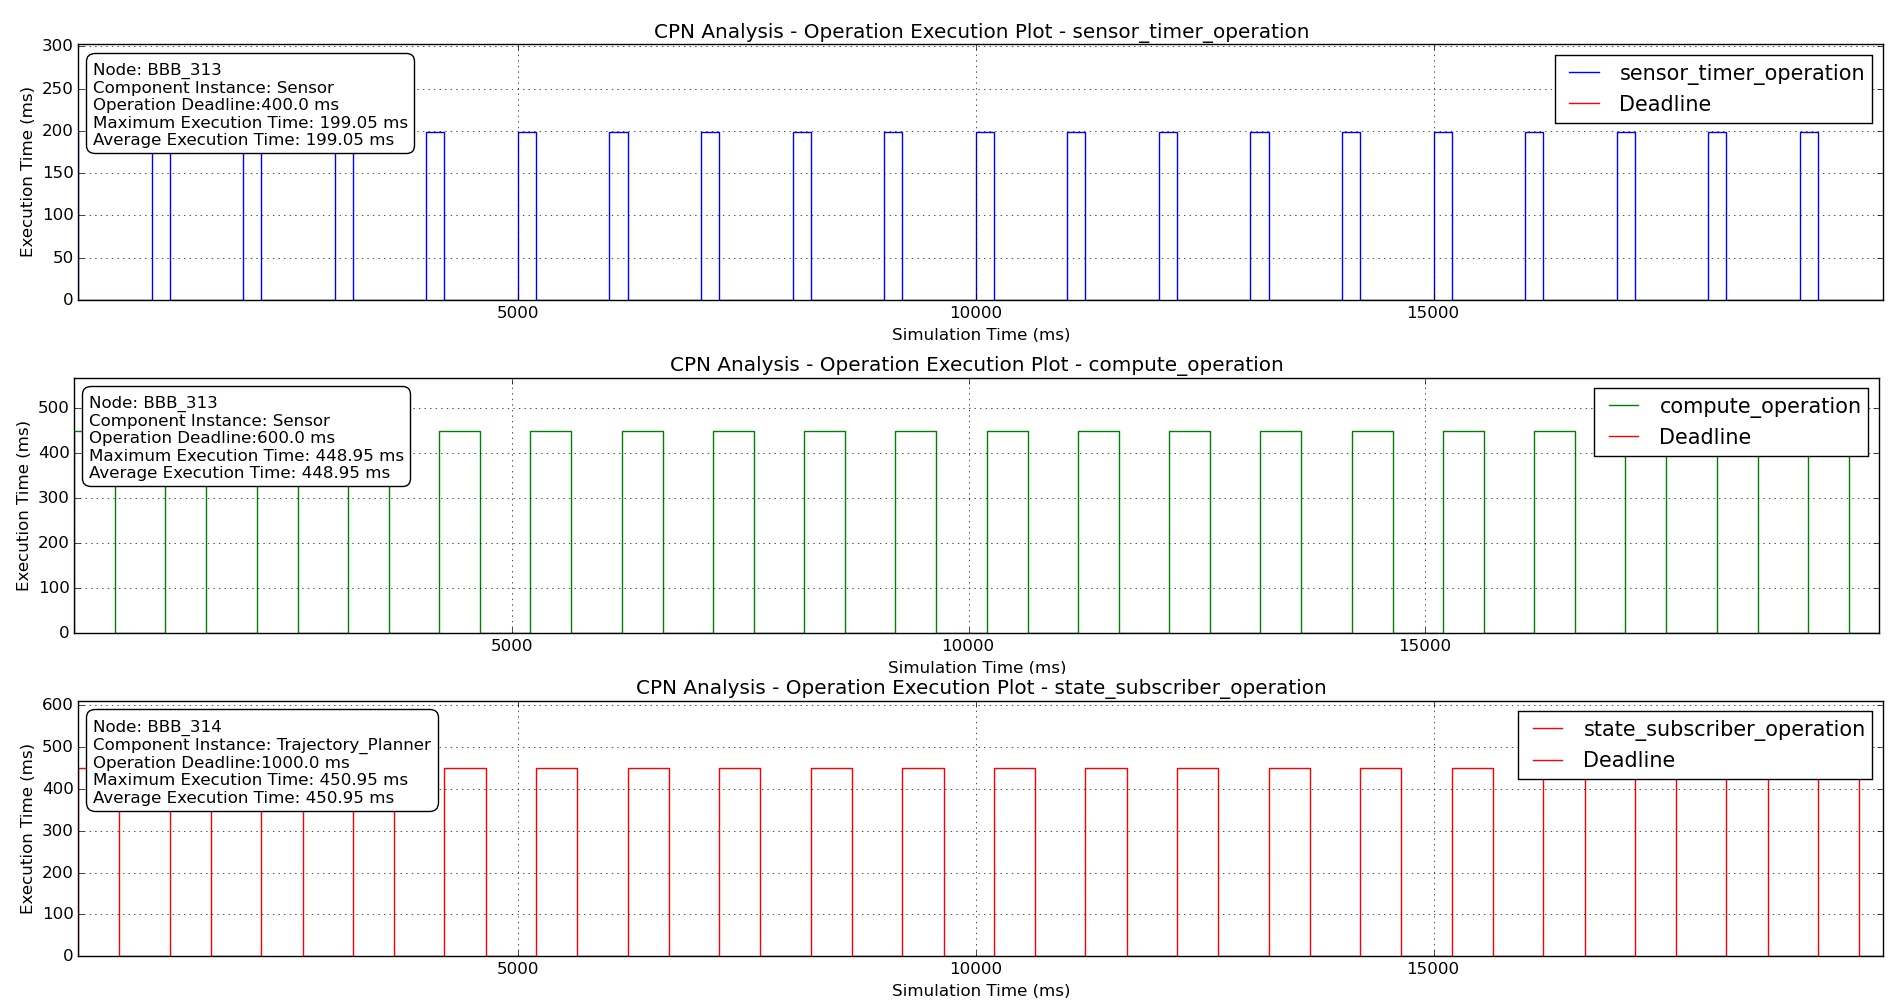
\includegraphics[width=\textwidth]{trajectory-planner-cpn}
	\caption{CPN Analysis Results: Trajectory Planner}
	\label{fig:trajectory-planner-cpn}
\end{figure}
\FloatBarrier

\begin{table}[]
	\centering
	\caption{Trajectory Planner Example -- Summary of Results}
	\label{tbl:trajectory-planner}
	\begin{tabular}{|c|c|c|c|c|}
		\hline
		\textbf{\begin{tabular}[c]{@{}c@{}}Operation\\ Name\end{tabular}} & \textbf{\begin{tabular}[c]{@{}c@{}}Component\\ Name\end{tabular}} & \textbf{\begin{tabular}[c]{@{}c@{}}Experimental\\ WCRT (ms)\end{tabular}} & \textbf{\begin{tabular}[c]{@{}c@{}}Timing Analysis\\ WCRT (ms)\end{tabular}} & \textbf{\begin{tabular}[c]{@{}c@{}}Deadline\\ (ms)\end{tabular}} \\ \hline
		\begin{tabular}[c]{@{}c@{}}Sensor\\ Timer\\ Operation\end{tabular} & Sensor & 199.00875 & 199.05 & 400 \\ \hline
		\begin{tabular}[c]{@{}c@{}}Compute\\ Operation\end{tabular} & Sensor & 445.373417 & 448.95 & 600 \\ \hline
		\begin{tabular}[c]{@{}c@{}}State\\ Subscriber\\ Operation\end{tabular} & \begin{tabular}[c]{@{}c@{}}Trajectory\\ Planner\end{tabular} & 446.874334 & 450.95 & 1000 \\ \hline
	\end{tabular}
\end{table}

If the sensor update frequency is increased to 100 ms, the sensor begins to notify the planner at a much higher frequency than expected. If there is no down-sampling on the planner's side, every single update will be handled by the planner, leading to dangerous queue size growth on the planner. Figure \ref{fig:trajectory-planner-bad-case} shows this deployment, as observed in the CPN analysis. 

\begin{figure}[h]
	\centering
	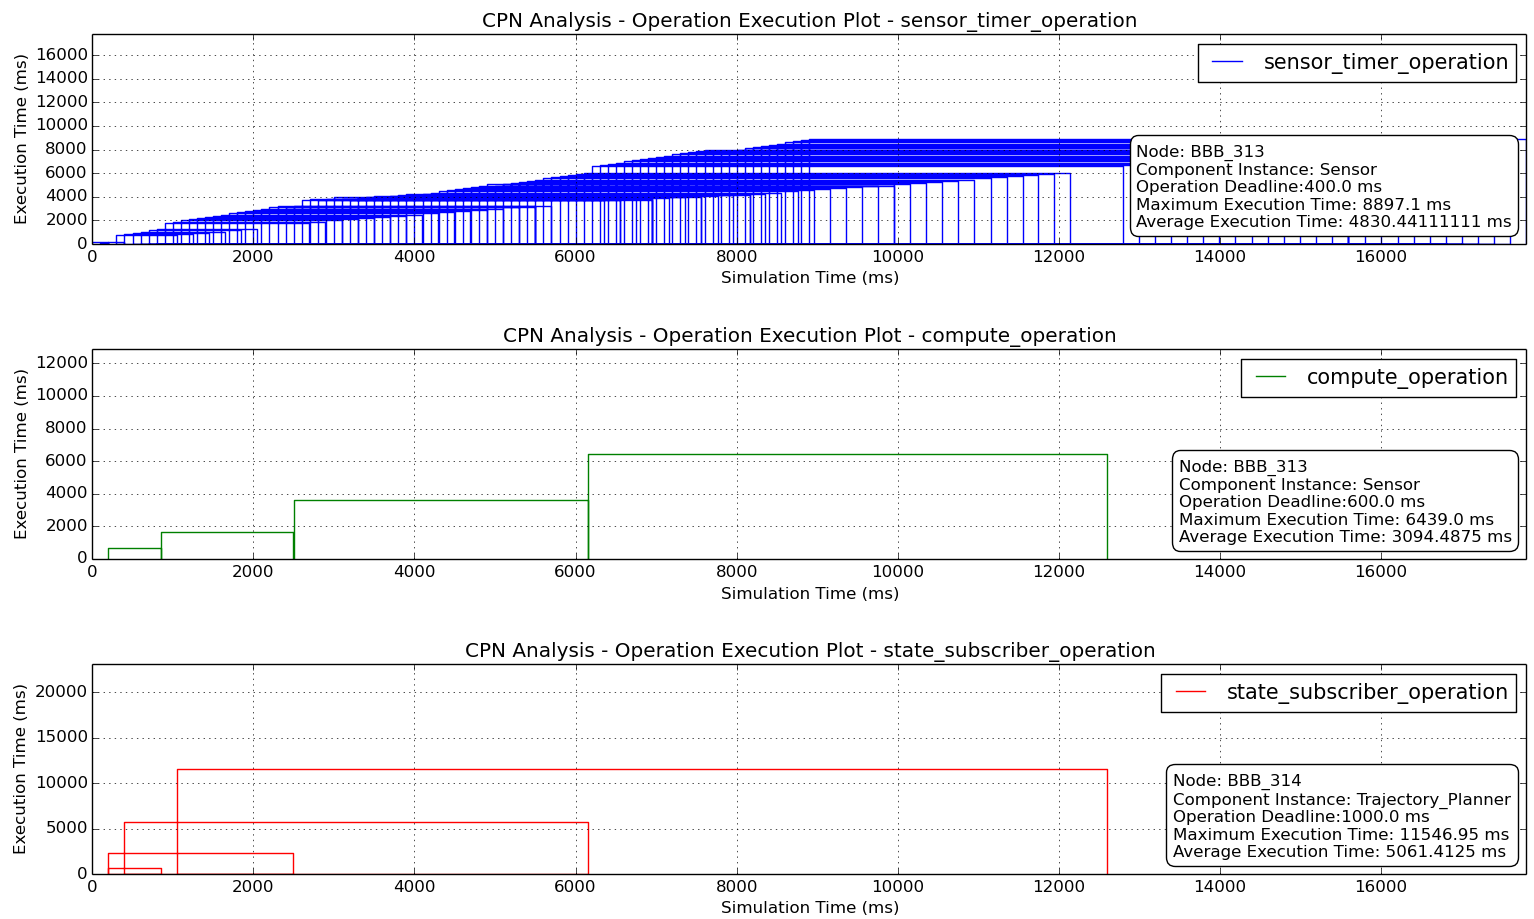
\includegraphics[width=\textwidth]{trajectory-planner-bad-case}
	\caption{CPN Analysis - Sensor firing too frequently}
	\label{fig:trajectory-planner-bad-case}
\end{figure}
\FloatBarrier

\subsection{Time-triggered Operations}

Time-triggered operations are an integral part of our component model. DREMS components are dormant by default. A timer has to trigger a inactive component for all subsequent interactions to happen. Since the DREMS component model supports various scheduling schemes on a single component message queue, this following test evaluates a priority first-in first-out (PFIFO) scheme. Multiple timers are created in a single component, each with a unique priority and period. A timer with a high frequency is assigned a high priority. Figure \ref{fig:periodic-timers} shows our experimental observations on a 5-timer example. 

Since ROSMOD components are associated with a single executor thread and component operations are also non-preemptive, a low-priority operation could theoretically run forever, starving a higher priority operation from ever executing, leading to deadline violations e.g. \emph{Timer\_1\_operation} can affect all other higher priority timers. Figure \ref{fig:periodic-timers-cpn} shows our CPN prediction where such a scenario is evident. It can be seen that \emph{Timer\_5\_operation}, the timer with the highest priority is periodically seeing spikes in execution time, courtesy of other lower priority operations consuming CPU without preemption. Table \ref{tbl:periodic-timers} summarizes the results.

\begin{figure}[h]
	\centering
	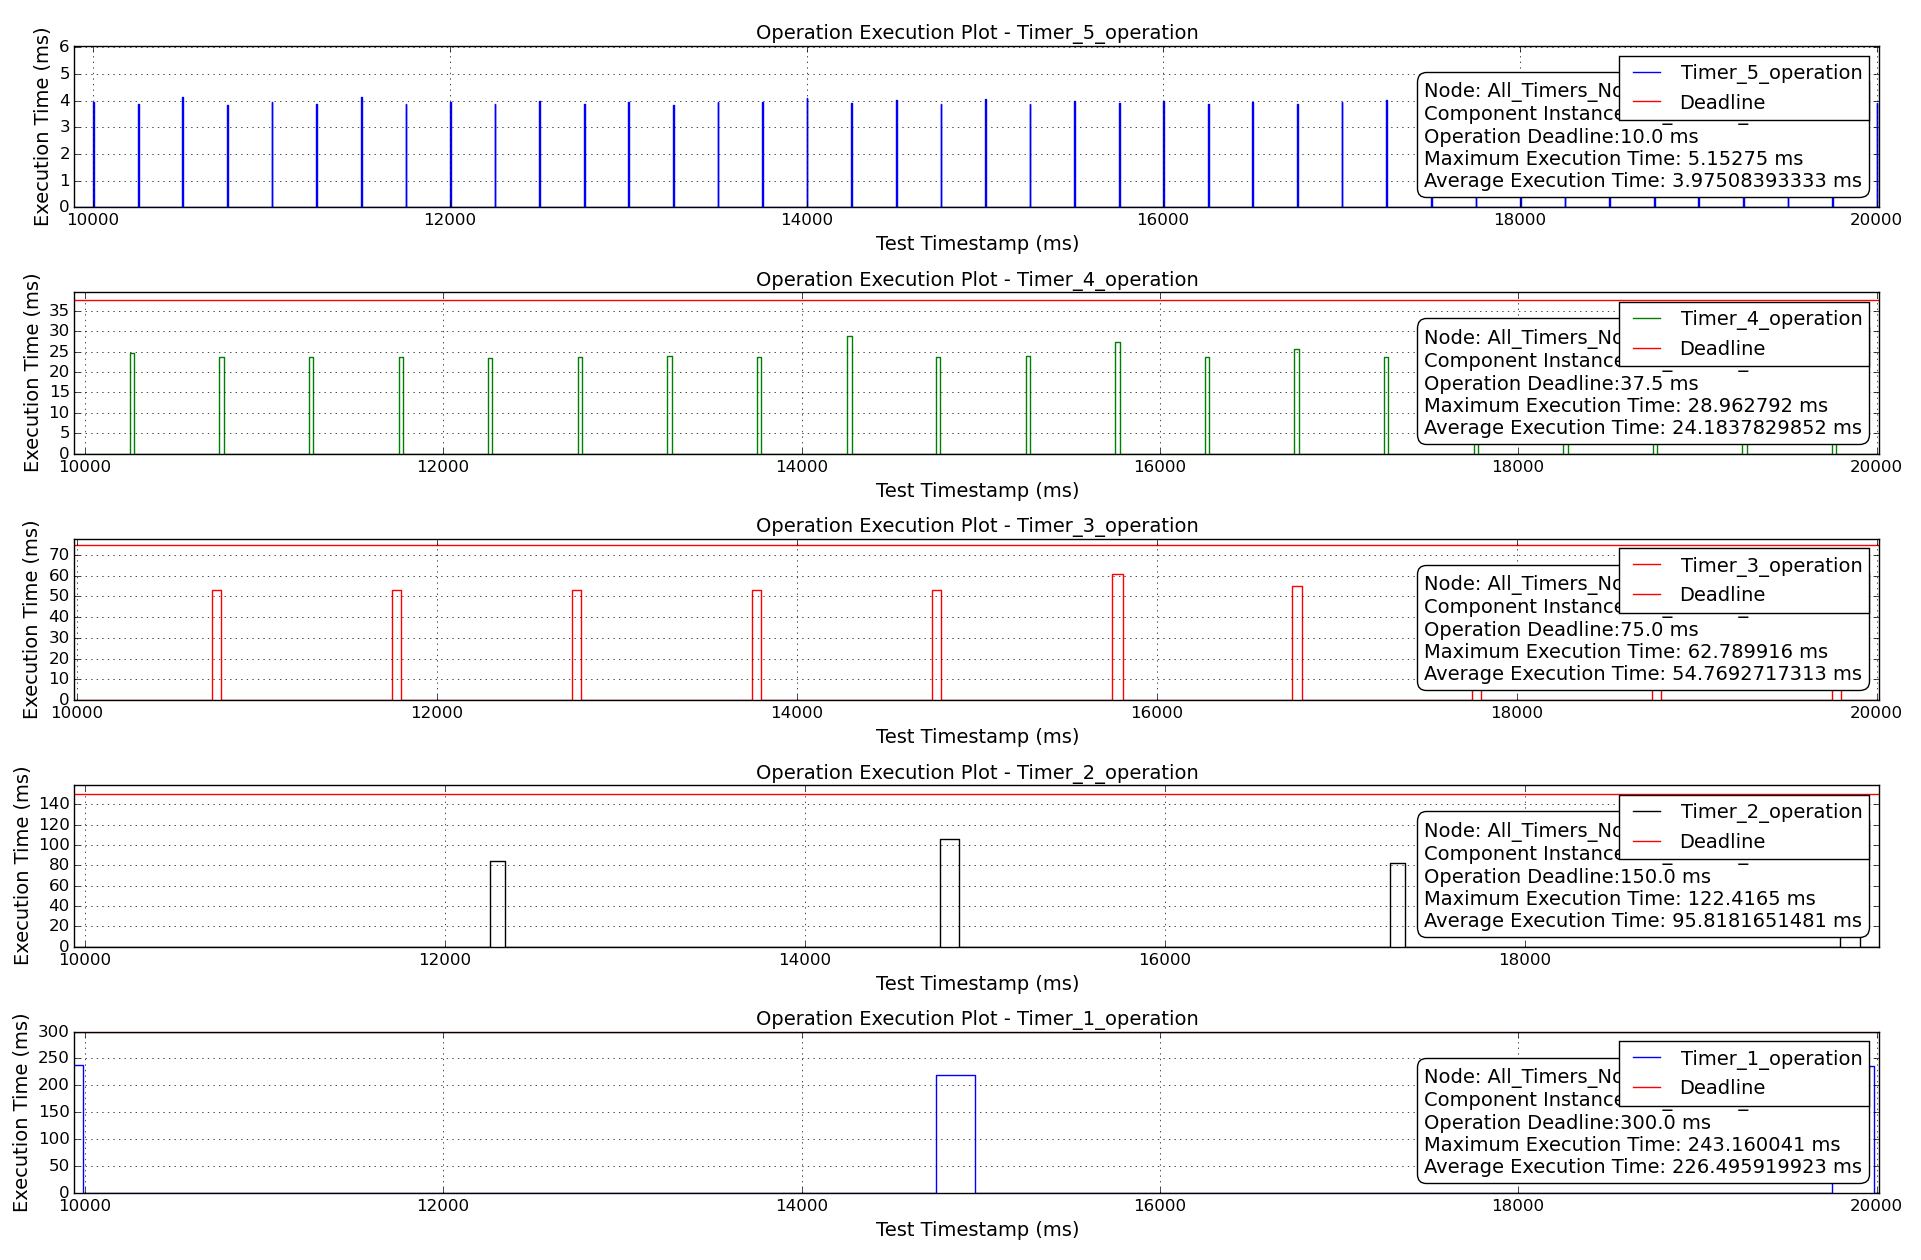
\includegraphics[width=\textwidth]{periodic-timers}
	\caption{Experimental Observation: Periodic Timers}
	\label{fig:periodic-timers}
\end{figure}
\FloatBarrier

\begin{figure}[h]
	\centering
	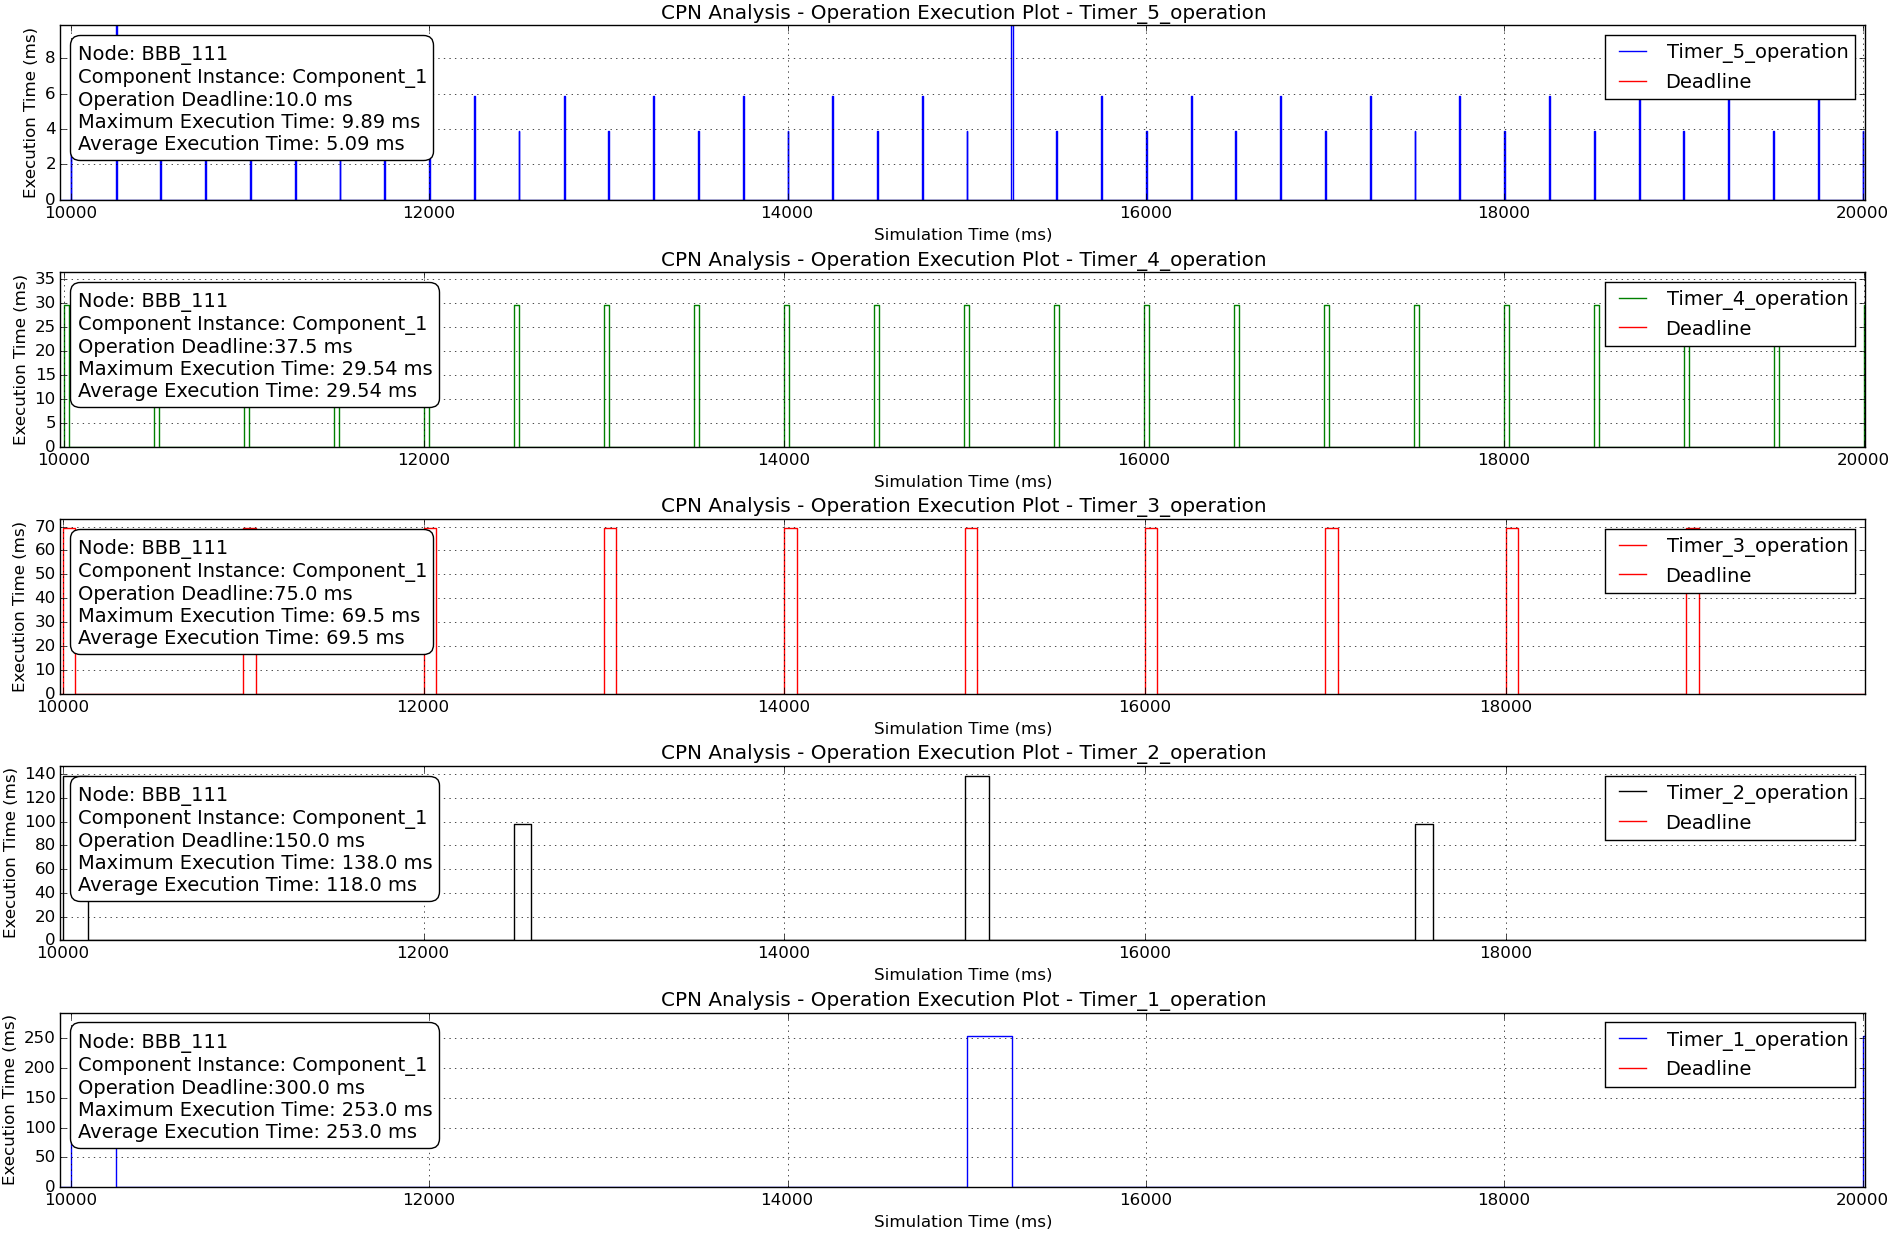
\includegraphics[width=\textwidth]{periodic-timers-cpn}
	\caption{CPN Analysis Results: Periodic Timers}
	\label{fig:periodic-timers-cpn}
\end{figure}
\FloatBarrier

\begin{table}[]
	\centering
	\caption{Periodic Timers -- Summary of Results}
	\label{tbl:periodic-timers}
	\begin{tabular}{|c|c|c|c|c|}
		\hline
		\textbf{\begin{tabular}[c]{@{}c@{}}Operation\\ Name\end{tabular}} & \textbf{\begin{tabular}[c]{@{}c@{}}Component\\ Name\end{tabular}} & \textbf{\begin{tabular}[c]{@{}c@{}}Experimental\\ WCRT (ms)\end{tabular}} & \textbf{\begin{tabular}[c]{@{}c@{}}Timing Analysis\\ WCRT (ms)\end{tabular}} & \textbf{\begin{tabular}[c]{@{}c@{}}Deadline\\ (ms)\end{tabular}} \\ \hline
		Timer\_1                                                          & Component\_1                                                      & 243.160041                                                                & 253.0                                                                        & 300                                                              \\ \hline
		Timer\_2                                                          & Component\_1                                                      & 122.4165                                                                  & 138.0                                                                        & 150                                                              \\ \hline
		Timer\_3                                                          & Component\_1                                                      & 62.789916                                                                 & 69.5                                                                         & 75                                                               \\ \hline
		Timer\_4                                                          & Component\_1                                                      & 28.962792                                                                 & 29.54                                                                        & 37.5                                                             \\ \hline
		Timer\_5                                                          & Component\_1                                                      & 5.15275                                                                   & 9.89                                                                         & 10                                                               \\ \hline
	\end{tabular}
\end{table}

\subsection{Long-Running Operations}
\label{sec:long_running_operations}

Our ROSMOD component model implements a non-preemptive component operation scheduling scheme. A component operation that is in the queue, regardless of its priority, must wait for the currently executing operation to run to completion. This is a strict rule for operation scheduling and does not work best in all system designs e.g. in a long-running computation-intensive application, rejuvenating the executing operation periodically and restarting it at a previous checkpoint increases the likelihood of successfully completing the application execution. In applications executing long-running artificial intelligence (AI) search algorithms e.g. flight path planning algorithms, the computation should not hinder the prompt response requirements of highly critical operation requests such as sudden maneuver changes. Our ROSMOD component model does not support the \emph{cancellation} of long-running component operations to service other highly critical operations waiting in the queue. With a few minor modifications to our scheduling schemes, long running operations can, however, be suspended if a higher priority waiting operation requires service. With these additions, we are able to model and analyze component-based systems that support long-running operations, with checkpoints, enabling the novel integration of AI-type algorithms into our design and analysis framework. 

\subsubsection{Challenges}

One of the primary challenges here is to identify the semantics of a long-running component operation i.e. the scenarios under which the component operations scheduler suspends a cooperating long-running operation in favor of some other operation waiting in the queue. If a long-running computation is modeled as a sequence of execution steps with bounded checkpoints, then the operation would execute one step at a time and suspend at such checkpoints if necessary. An important challenge here is accurately identifying the priority difference between the long-running operation and the waiting operation. If the long-running operation is one checkpoint away from completion e.g. 100-200 ms of execution time, then strictly following our suspension rules would not be the most prudent choice since this operation is almost complete. However, if the waiting operation is a critical one, then regardless of the state of the long-running operation, the executing operation must be suspended. Secondly, the modeled long-running computation semantics must be incorporated into our component model so that any analysis results obtained can be suitably validated. 

\begin{figure}[h]
	\centering
	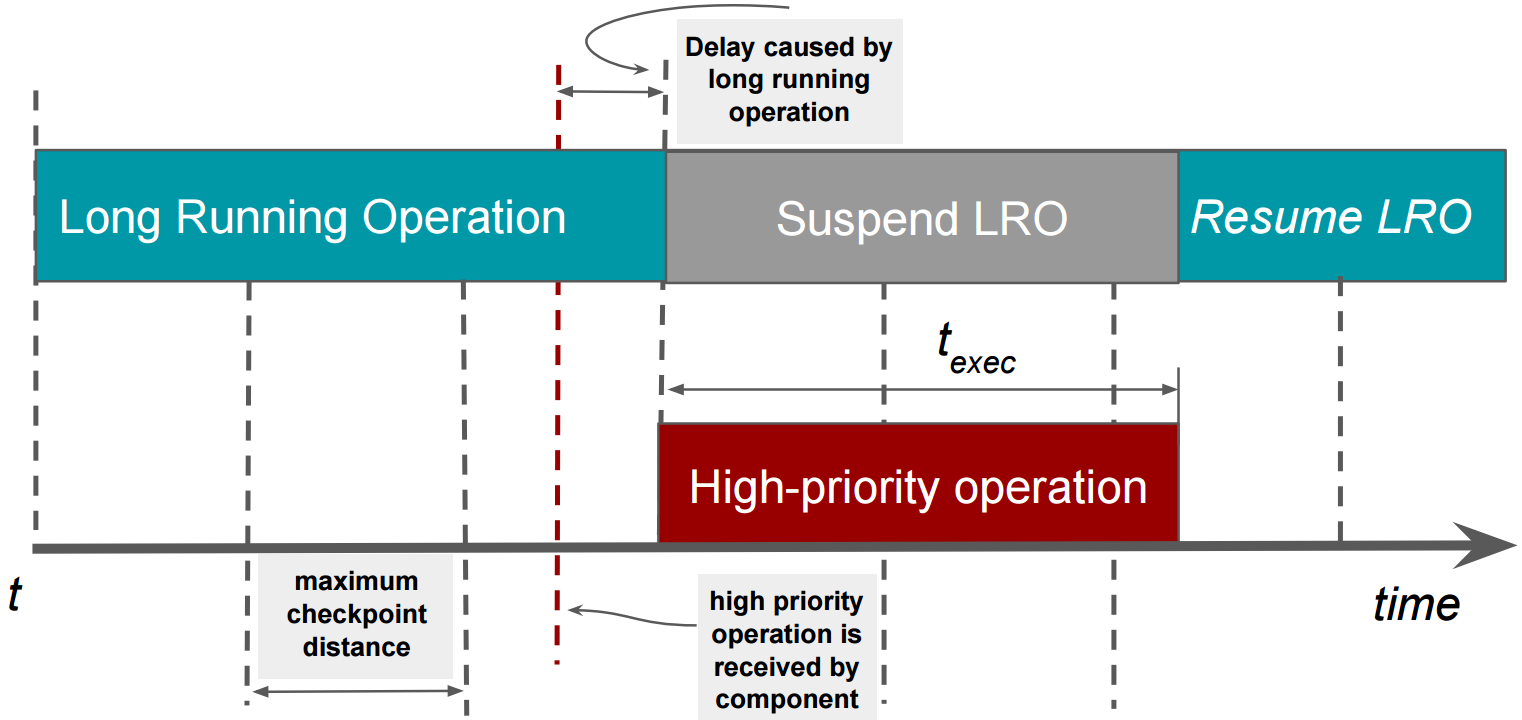
\includegraphics[width=\textwidth]{lro-semantics}
	\caption{Long Running Operations - Timing Diagram}
	\label{fig:lro-semantics}
\end{figure}
\FloatBarrier

\subsubsection{Implementation and Results}

In each long-running operation, we, therefore, include a synchronous \emph{checkpoint step}, as shown in Figure \ref{fig:lro-semantics}. The only assumption we make about this long-running operation is the periodicity of these checkpoint steps i.e. we know how frequently a new checkpoint is reached and we assume that the search algorithm used by the long-running operation is capable of reaching a safe state (the checkpoint) before suspending itself if required. If a higher priority operation is ready and waiting in the queue, the long-running operation runs till the next checkpoint is reached, then suspends. The higher priority operation is then processed. Figure \ref{fig:three-components-lro-rosmod} shows the \emph{Software Model} for a component assembly with long running operations.

\begin{figure}[h]
	\centering
	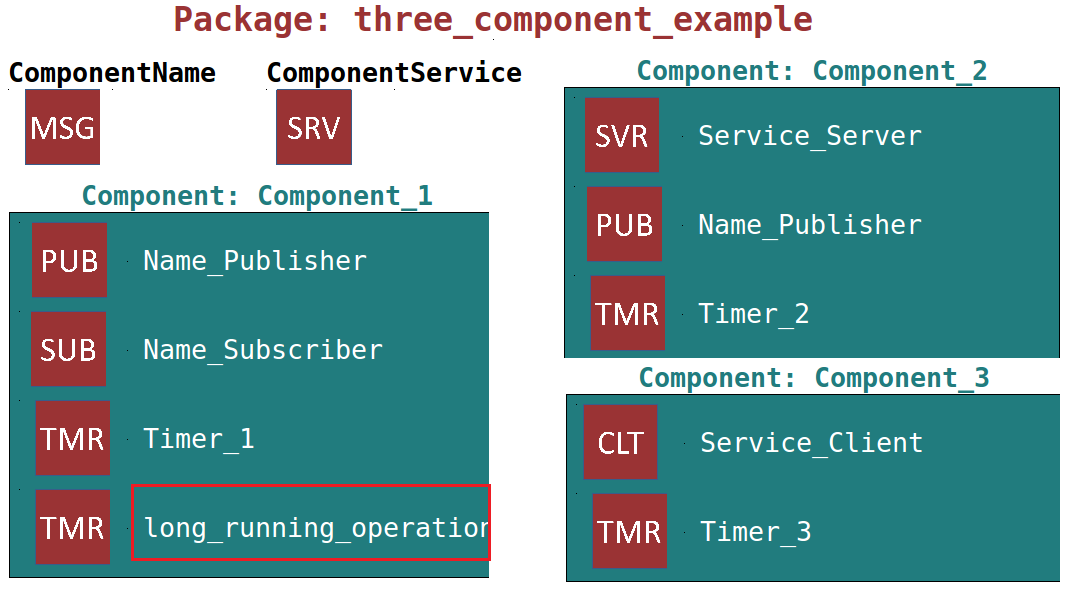
\includegraphics[width=\textwidth]{three-components-lro-rosmod}
	\caption{Long Running Operation - Software Model}
	\label{fig:three-components-lro-rosmod}
\end{figure}
\FloatBarrier

The assembly consists of three components. Components \emph{Component\_1} and \emph{Component\_2} periodically publish on the \emph{ComponentName} message. \emph{Component\_3} periodically queries the server in \emph{Component\_2}. During these interactions, \emph{Component\_1} is performing a long running operation, the duration of which, is magnitudes larger than the average execution time of all other operations. Figure \ref{fig:three-components-lro} shows the execution time plot of this scenario, as measured on our testbed. 

\begin{figure}[h]
	\centering
	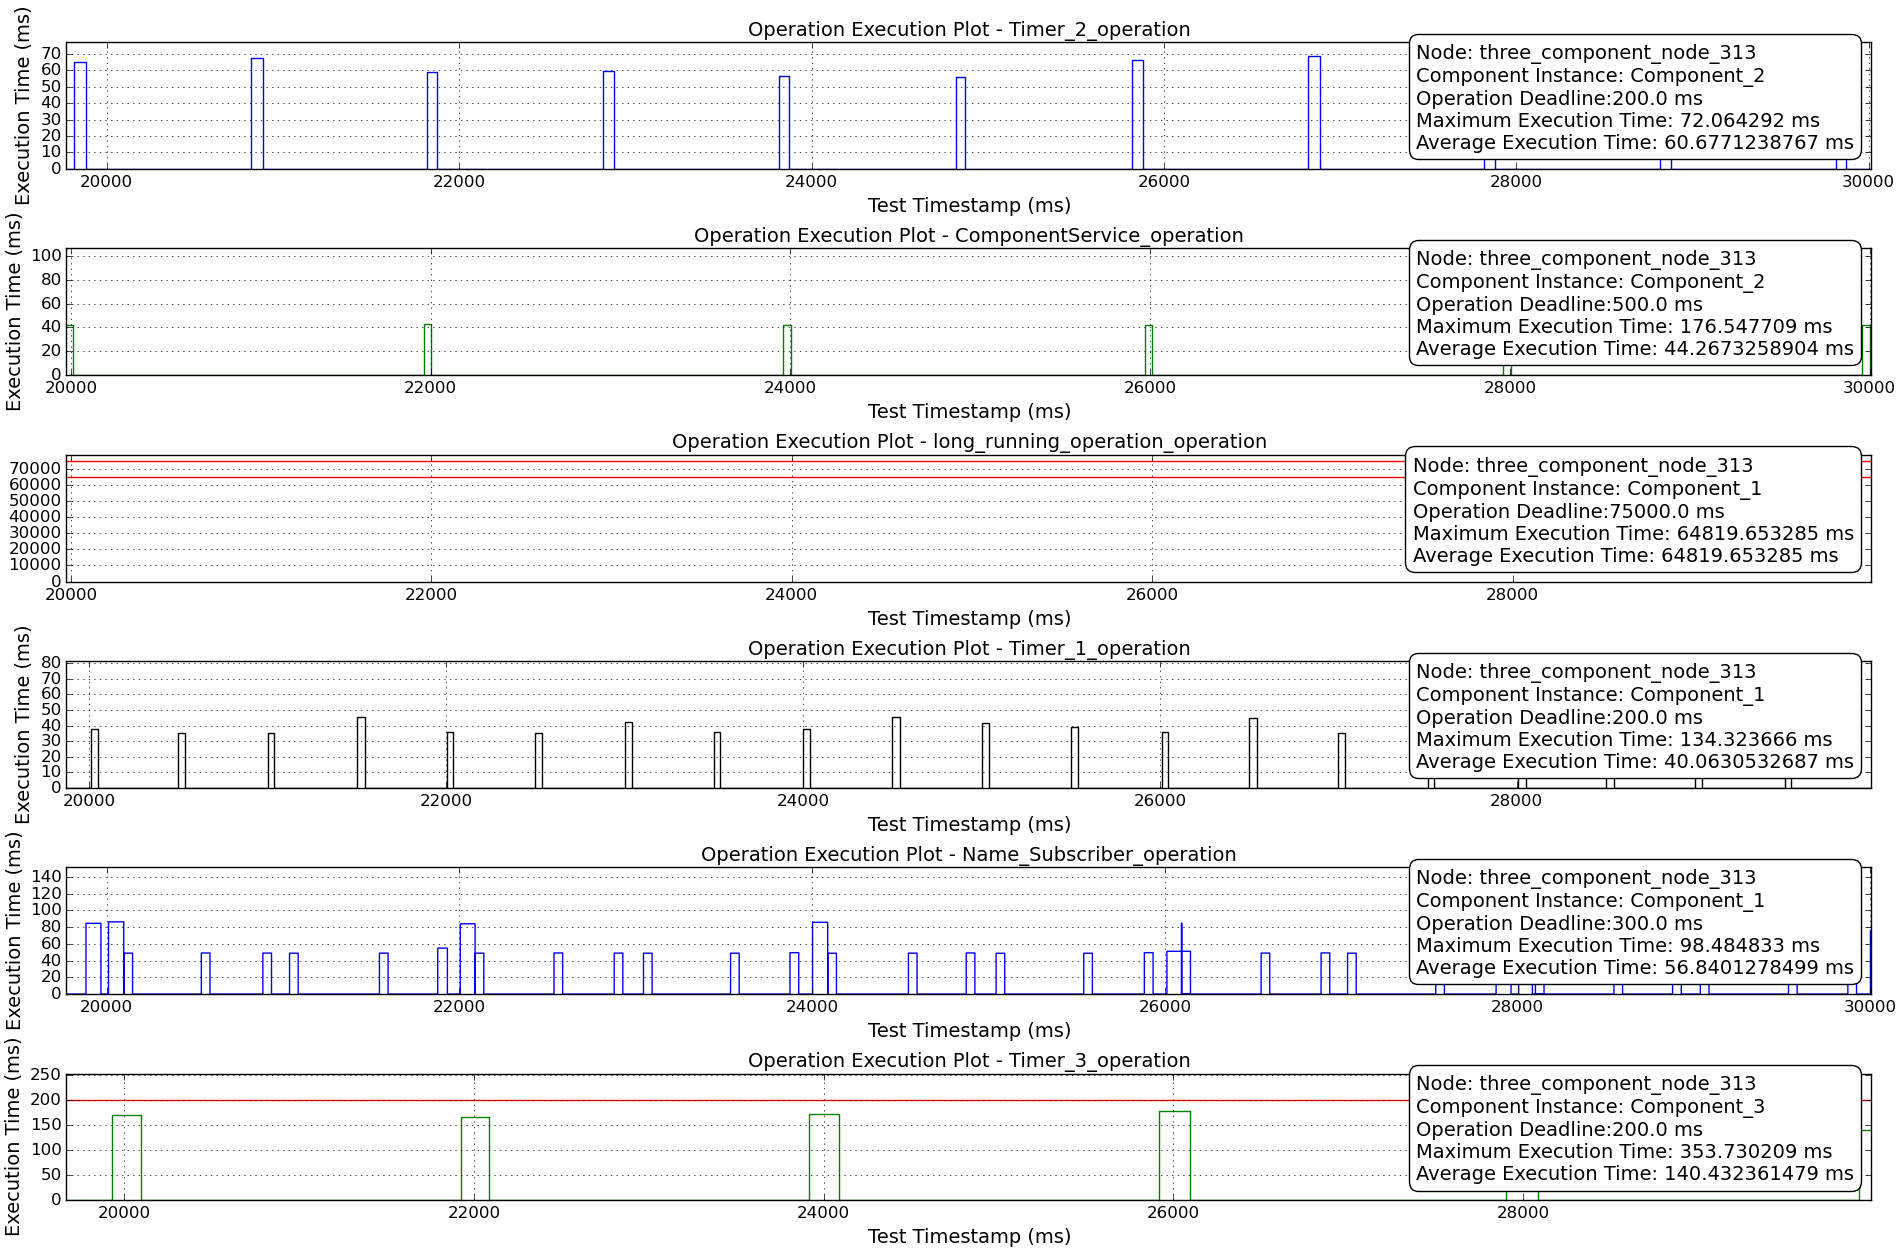
\includegraphics[width=\textwidth]{three-components-lro}
	\caption{Experimental Observation: Composed Component Assembly}
	\label{fig:three-components-lro}
\end{figure}
\FloatBarrier

For the CPN analysis, in order to obtain pure execution times of all these operations, each operation on each component is executed as a stand-alone function on the hardware. This way, we know the average and worst-case execution times of all operational steps with minimal interruptions. These numbers are injected into our generated CPN and state space analysis is performed. Figure \ref{fig:three-components-lro-cpn} shows our CPN analysis results for the same assembly.


\begin{figure}[h]
	\centering
	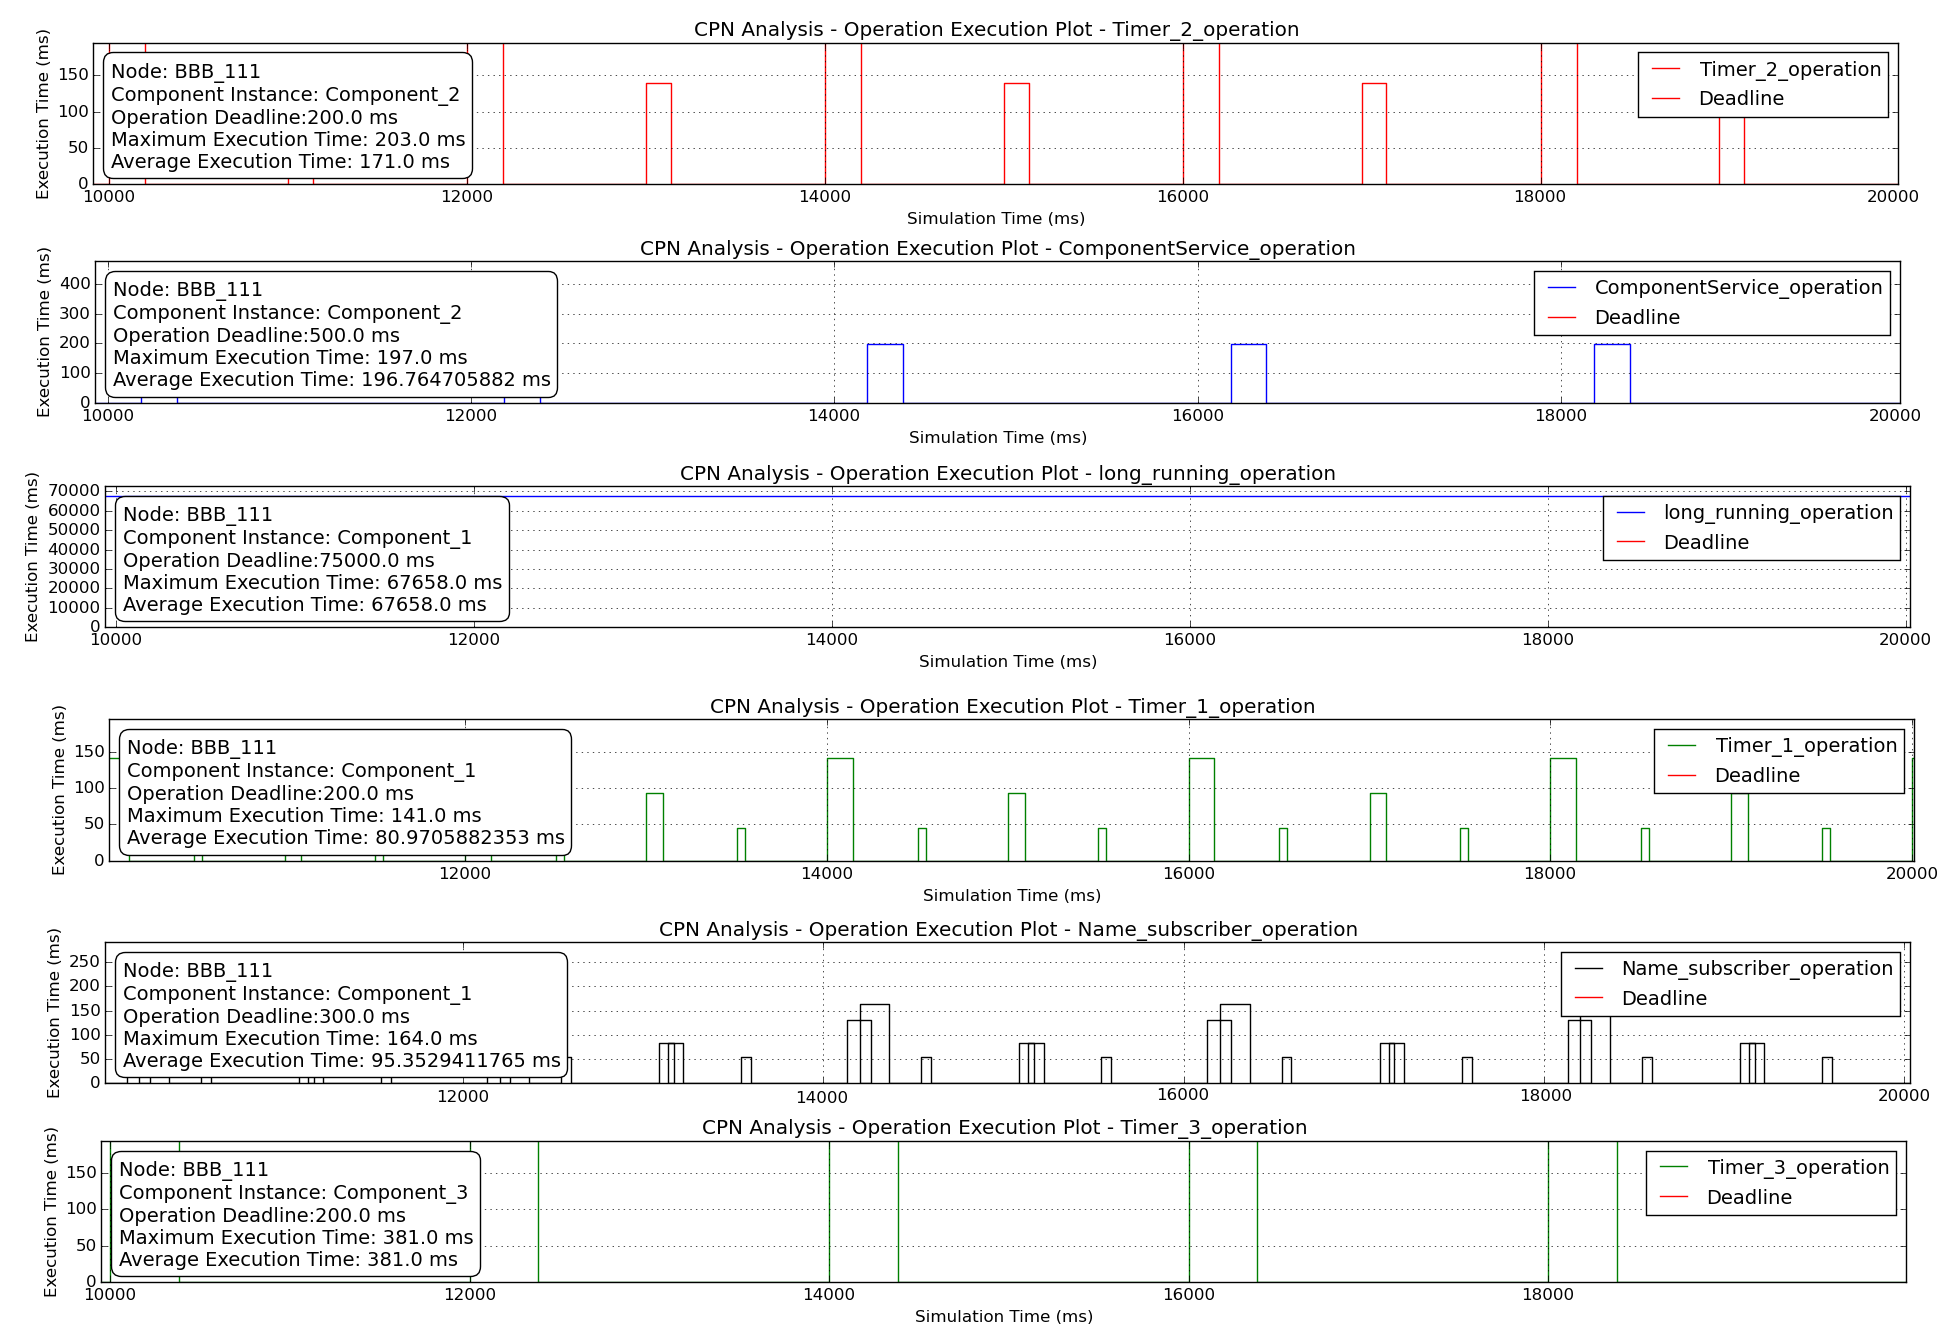
\includegraphics[width=\textwidth]{three-components-lro-cpn}
	\caption{CPN Analysis Results: Composed Component Assembly}
	\label{fig:three-components-lro-cpn}
\end{figure}
\FloatBarrier

\subsection{Integration with Physics Simulators - Cyber-Physical Systems Scenarios}

\subsubsection{Kerbal Space Program}

Kerbal Space Program \cite{KSP} (KSP) is a widely popular space flight simulator for a variety of platforms including Linux, OS X and Windows. In this game, players get to manage a space program, designing and building spacecrafts and exploring celestial bodies. 

While KSP does not provide a perfect simulation of reality, it has been widely praised for its component-based design and development process coupled with aerodynamic, gravitational, and rigid-body interaction and simulation. In this simulation, every man-made object follows Newtonian dynamics. Rocket thrust and aerodynamic forces are accurately applied to the vehicles based on the directions and precise positions in which the force-affected elements are mounted on the vessel. Using KSP, we have modeled scenarios for a variety of flight missions including interplanetary travel. In this section, we briefly describe an aircraft flight controller that was designed and tested using the RCPS testbed and KSP.

This CPS scenario is a flight controller application used to completely control a KSP aircraft from the primary space-plane hanger to a destination airport. The application processes require inputs from KSP e.g. sensor data about pitch, roll, yaw, mean altitude etc. and interfaces to control the flight dynamics e.g. thrust, pitch and heading. If these interfaces are setup, then the processes can periodically retrieve flight telemetry and provide commands for course correction and feedback control.


Using an open source project called kRPC \cite{kRPC} (Kerbal Remote Procedure Call Server), the BBB nodes running CPS processes are provided with an interface to the simulation. Figure \ref{fig:ksp} shows the Stearwing A300 aircraft taking off from the space-plane hanger and stabilizing at a cruising altitude of 2000 meters. Each control unit in the aircraft is simulated by a BBB. It is critical to incorporate redundancy in all components and connections to assure that the system can survive runtime failures, especially in airborne software \cite{airborne_software} \cite{kornecki2004approaches}. So, many of the RCPS nodes in our testbed act as redundant sensors, all connected to KSP, receiving and periodically publishing messages. If one of the nodes in the testbed fails, either due to a hardware anomaly or a software fault, then the rest of the nodes are used to arrive at a general agreement regarding the sensor value to be considered for control.

\begin{figure}[h]
	\centering
	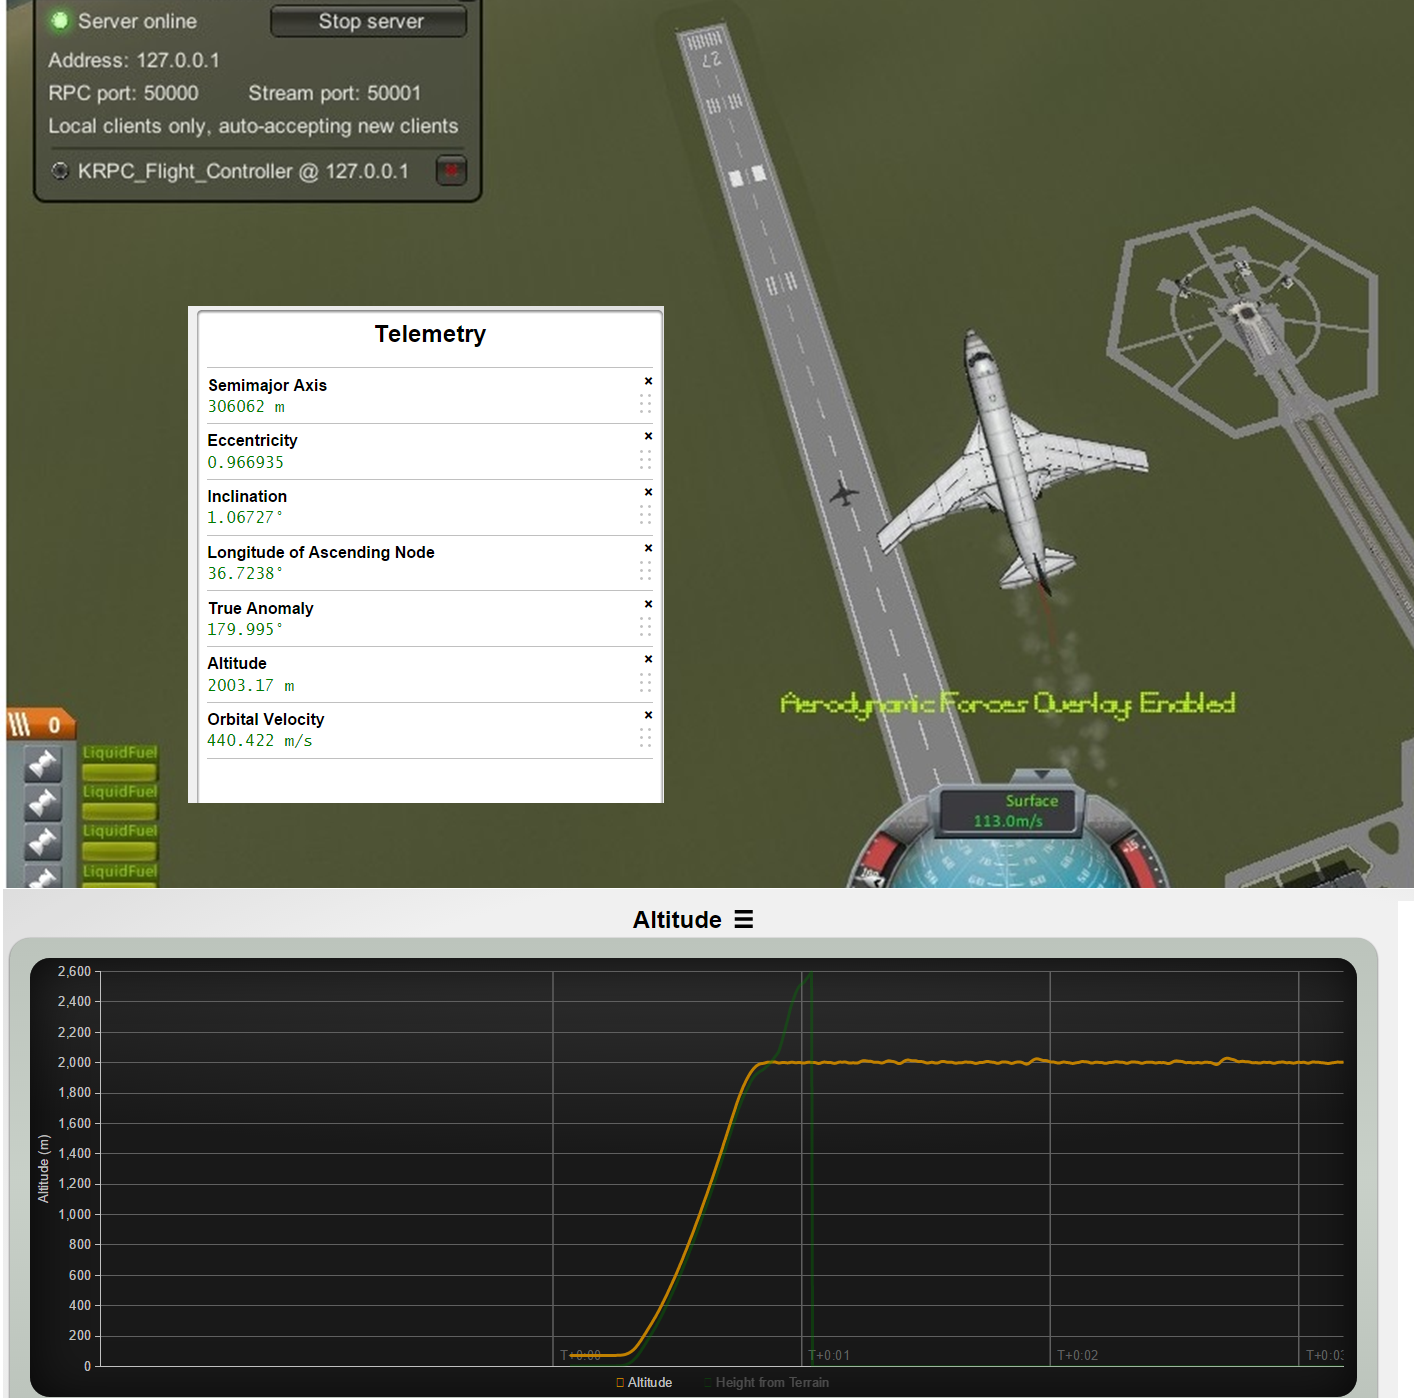
\includegraphics[width=\textwidth]{ksp}
	\caption{Stearwing A300 PID Control}
	\label{fig:ksp}
\end{figure} 
\FloatBarrier 

\subsubsection{Experimental Observations - Physics simulation on Server}

\begin{figure}[h]
	\centering
	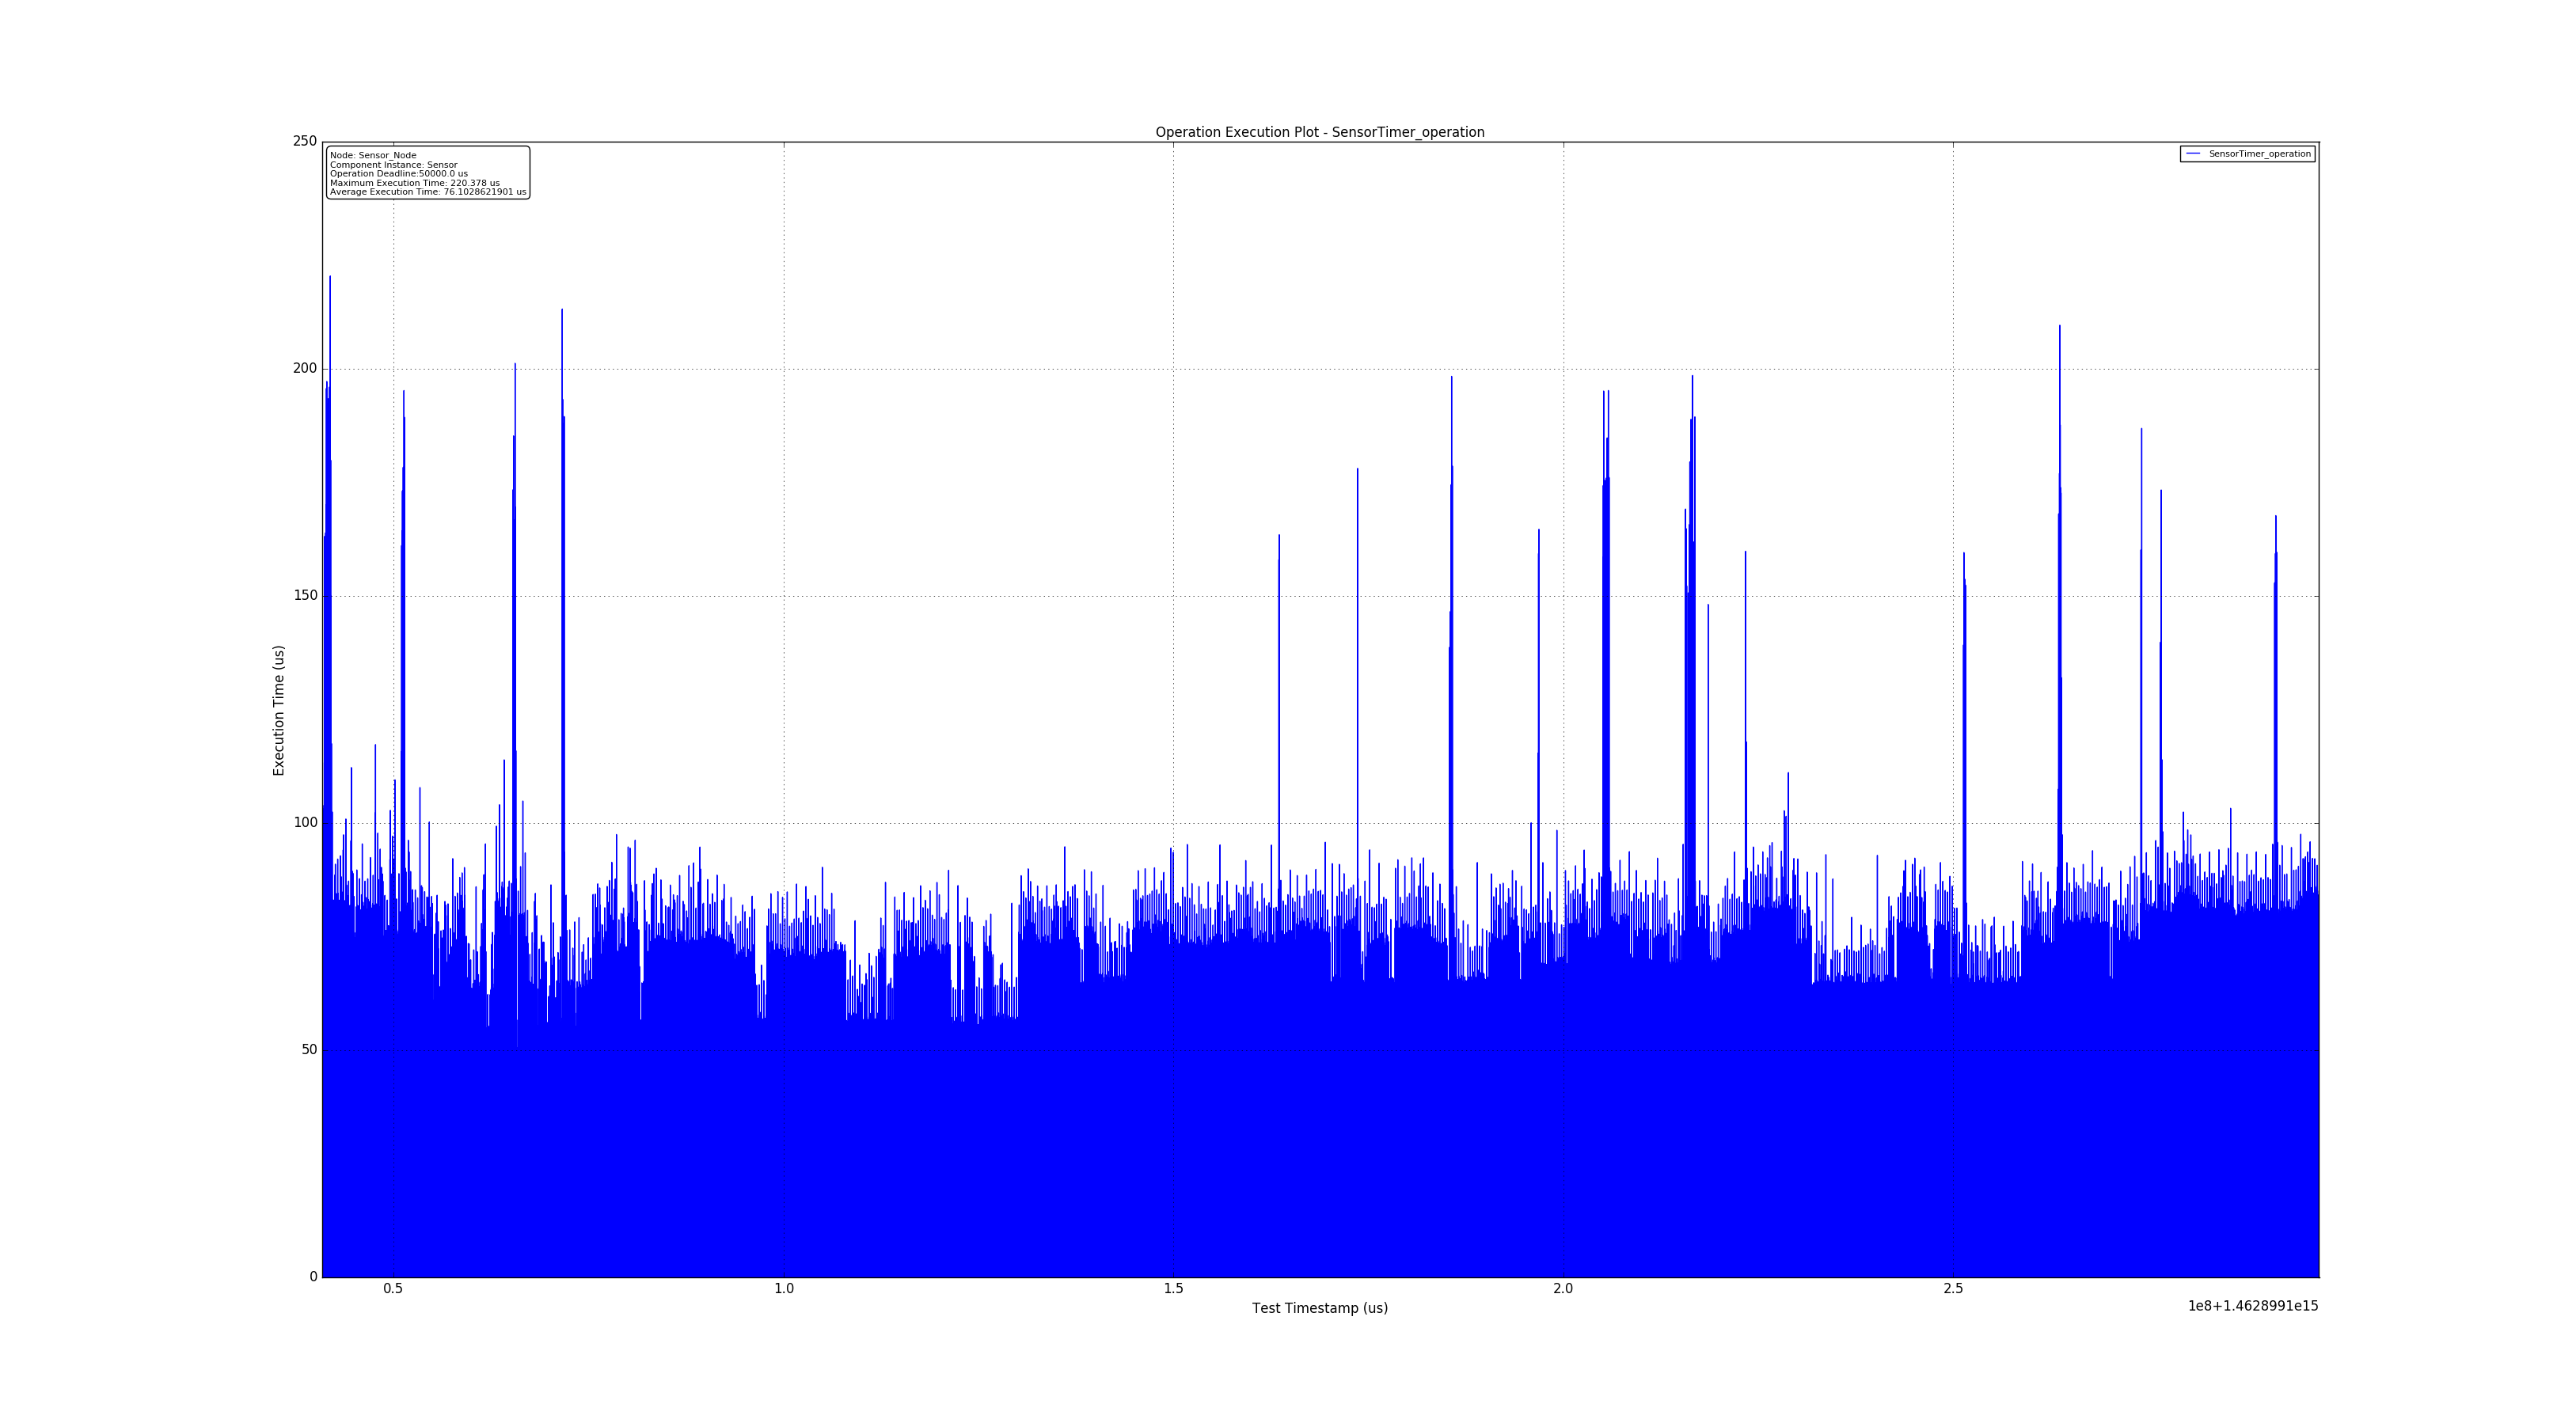
\includegraphics[width=\textwidth]{ksp_sensor}
	\caption{Stearwing Control - Sensor Component}
	\label{fig:sensor}
\end{figure} 
\FloatBarrier 

\begin{figure}[h]
	\centering
	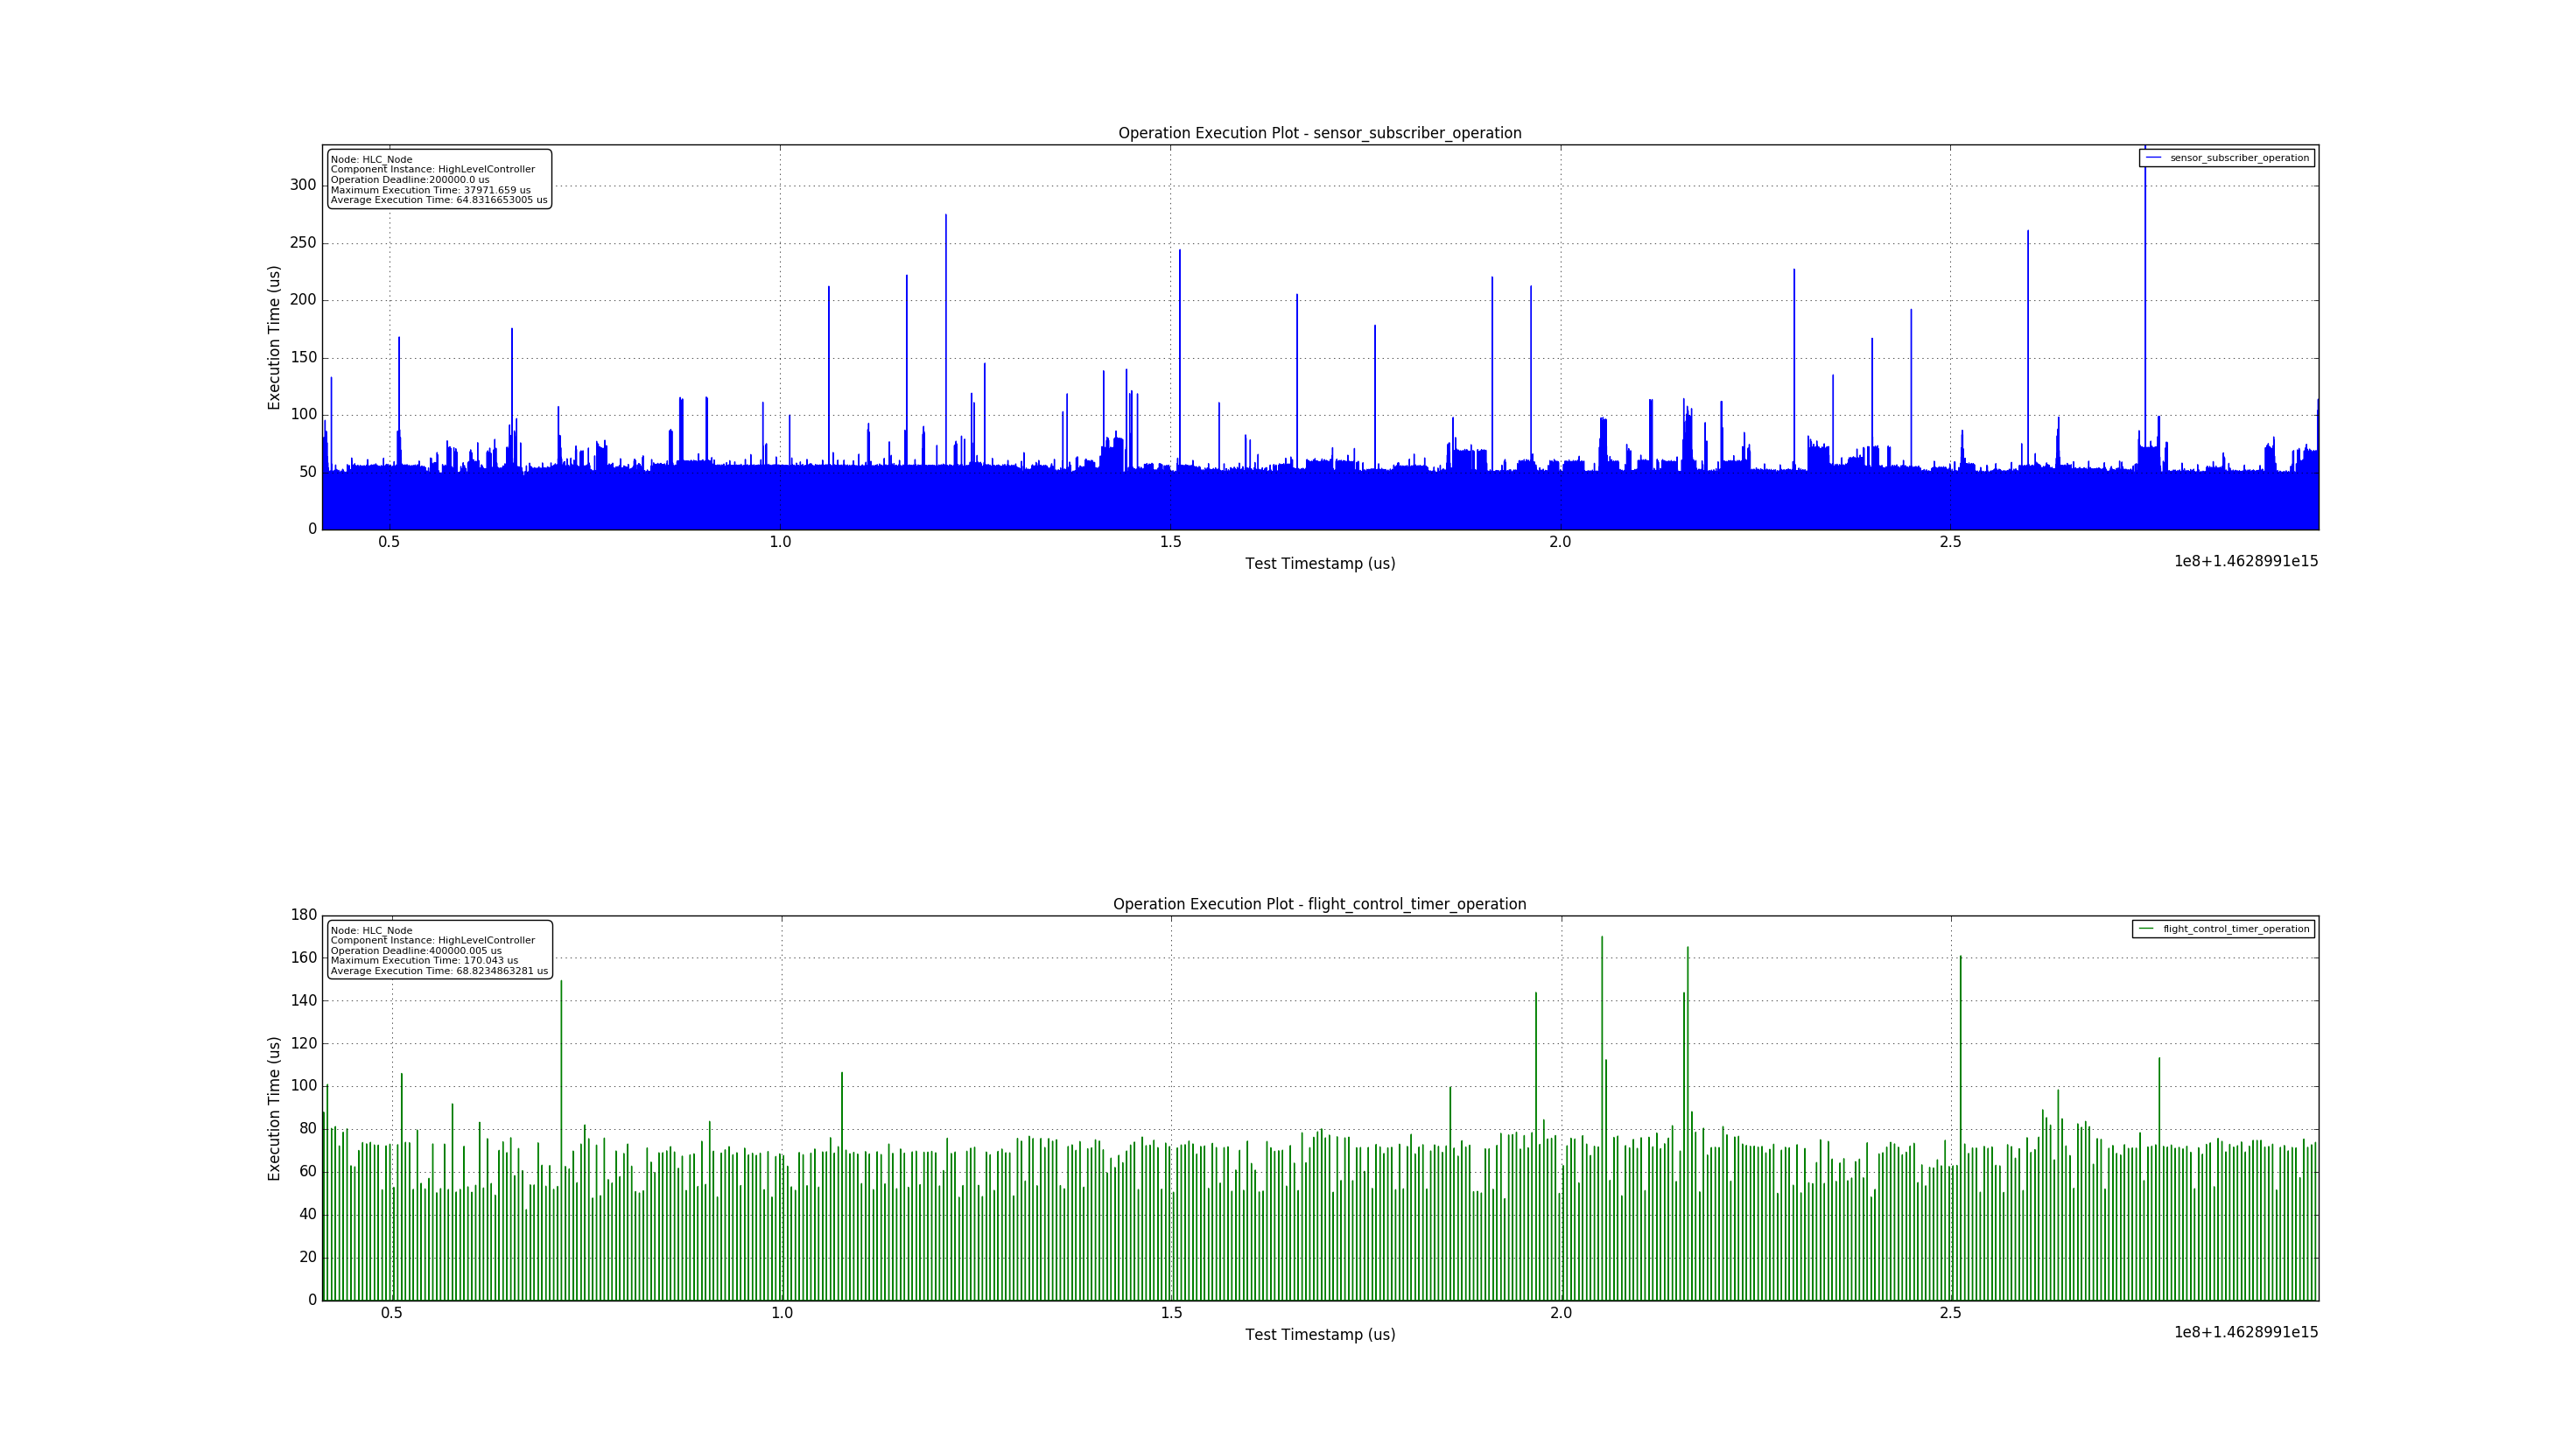
\includegraphics[width=\textwidth]{ksp_hlc}
	\caption{Stearwing Control - High-level Controller Component}
	\label{fig:ksp_hlc}
\end{figure} 
\FloatBarrier 

\begin{figure}[h]
	\centering
	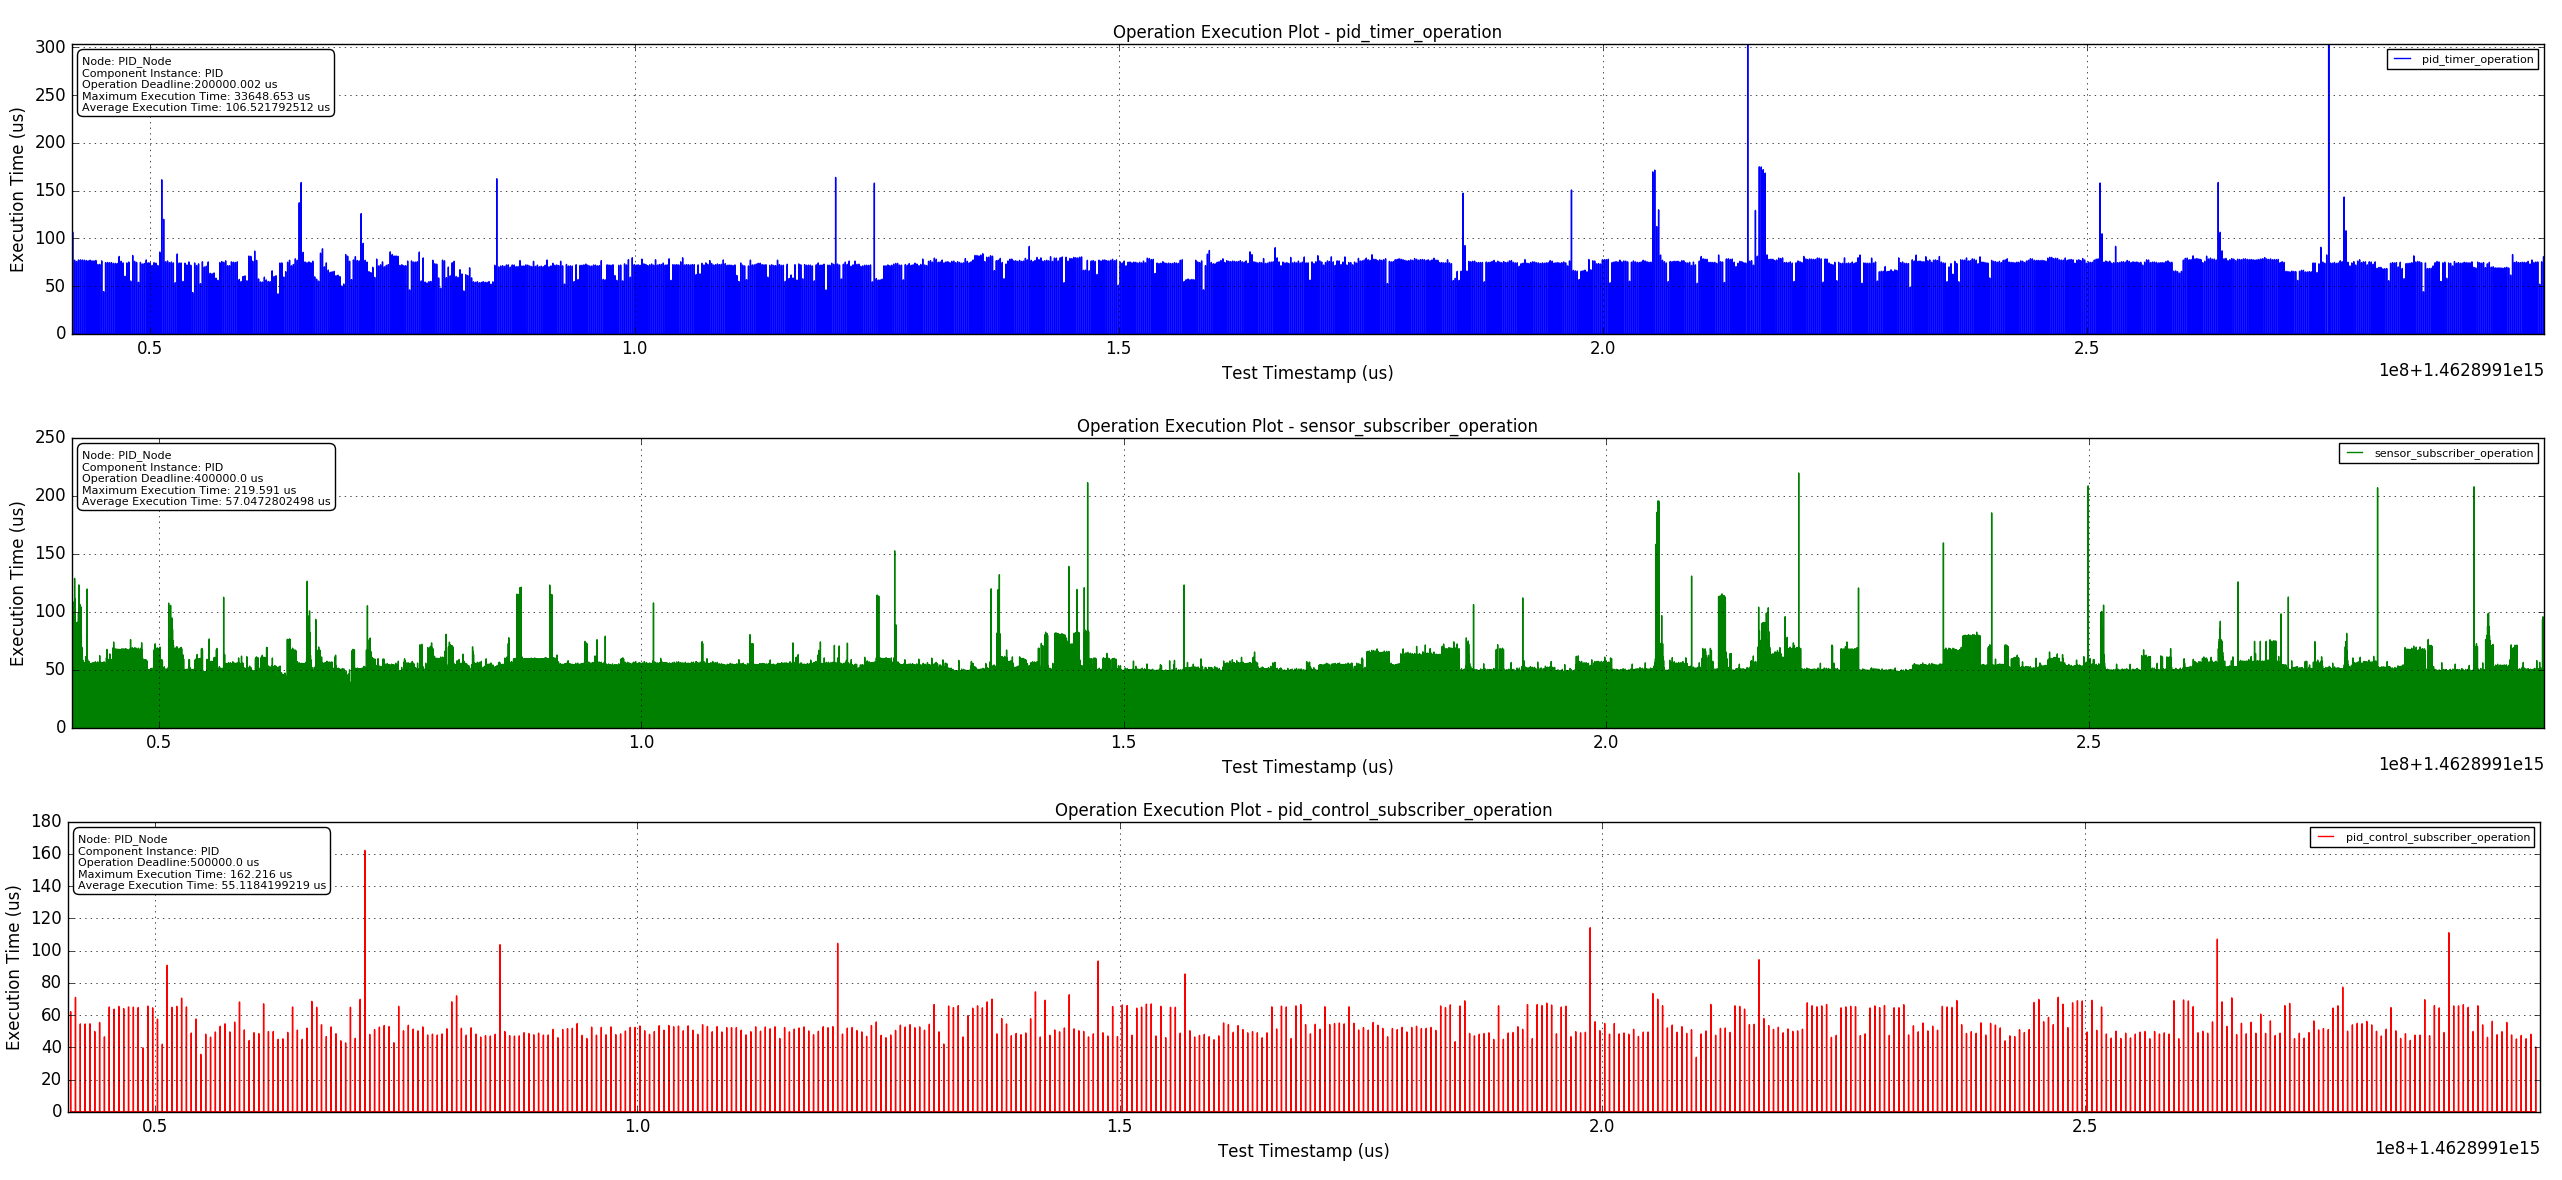
\includegraphics[width=\textwidth]{ksp_pid}
	\caption{Stearwing Control - PID Component}
	\label{fig:ksp_pid}
\end{figure} 
\FloatBarrier 

\begin{figure}[h]
	\centering
	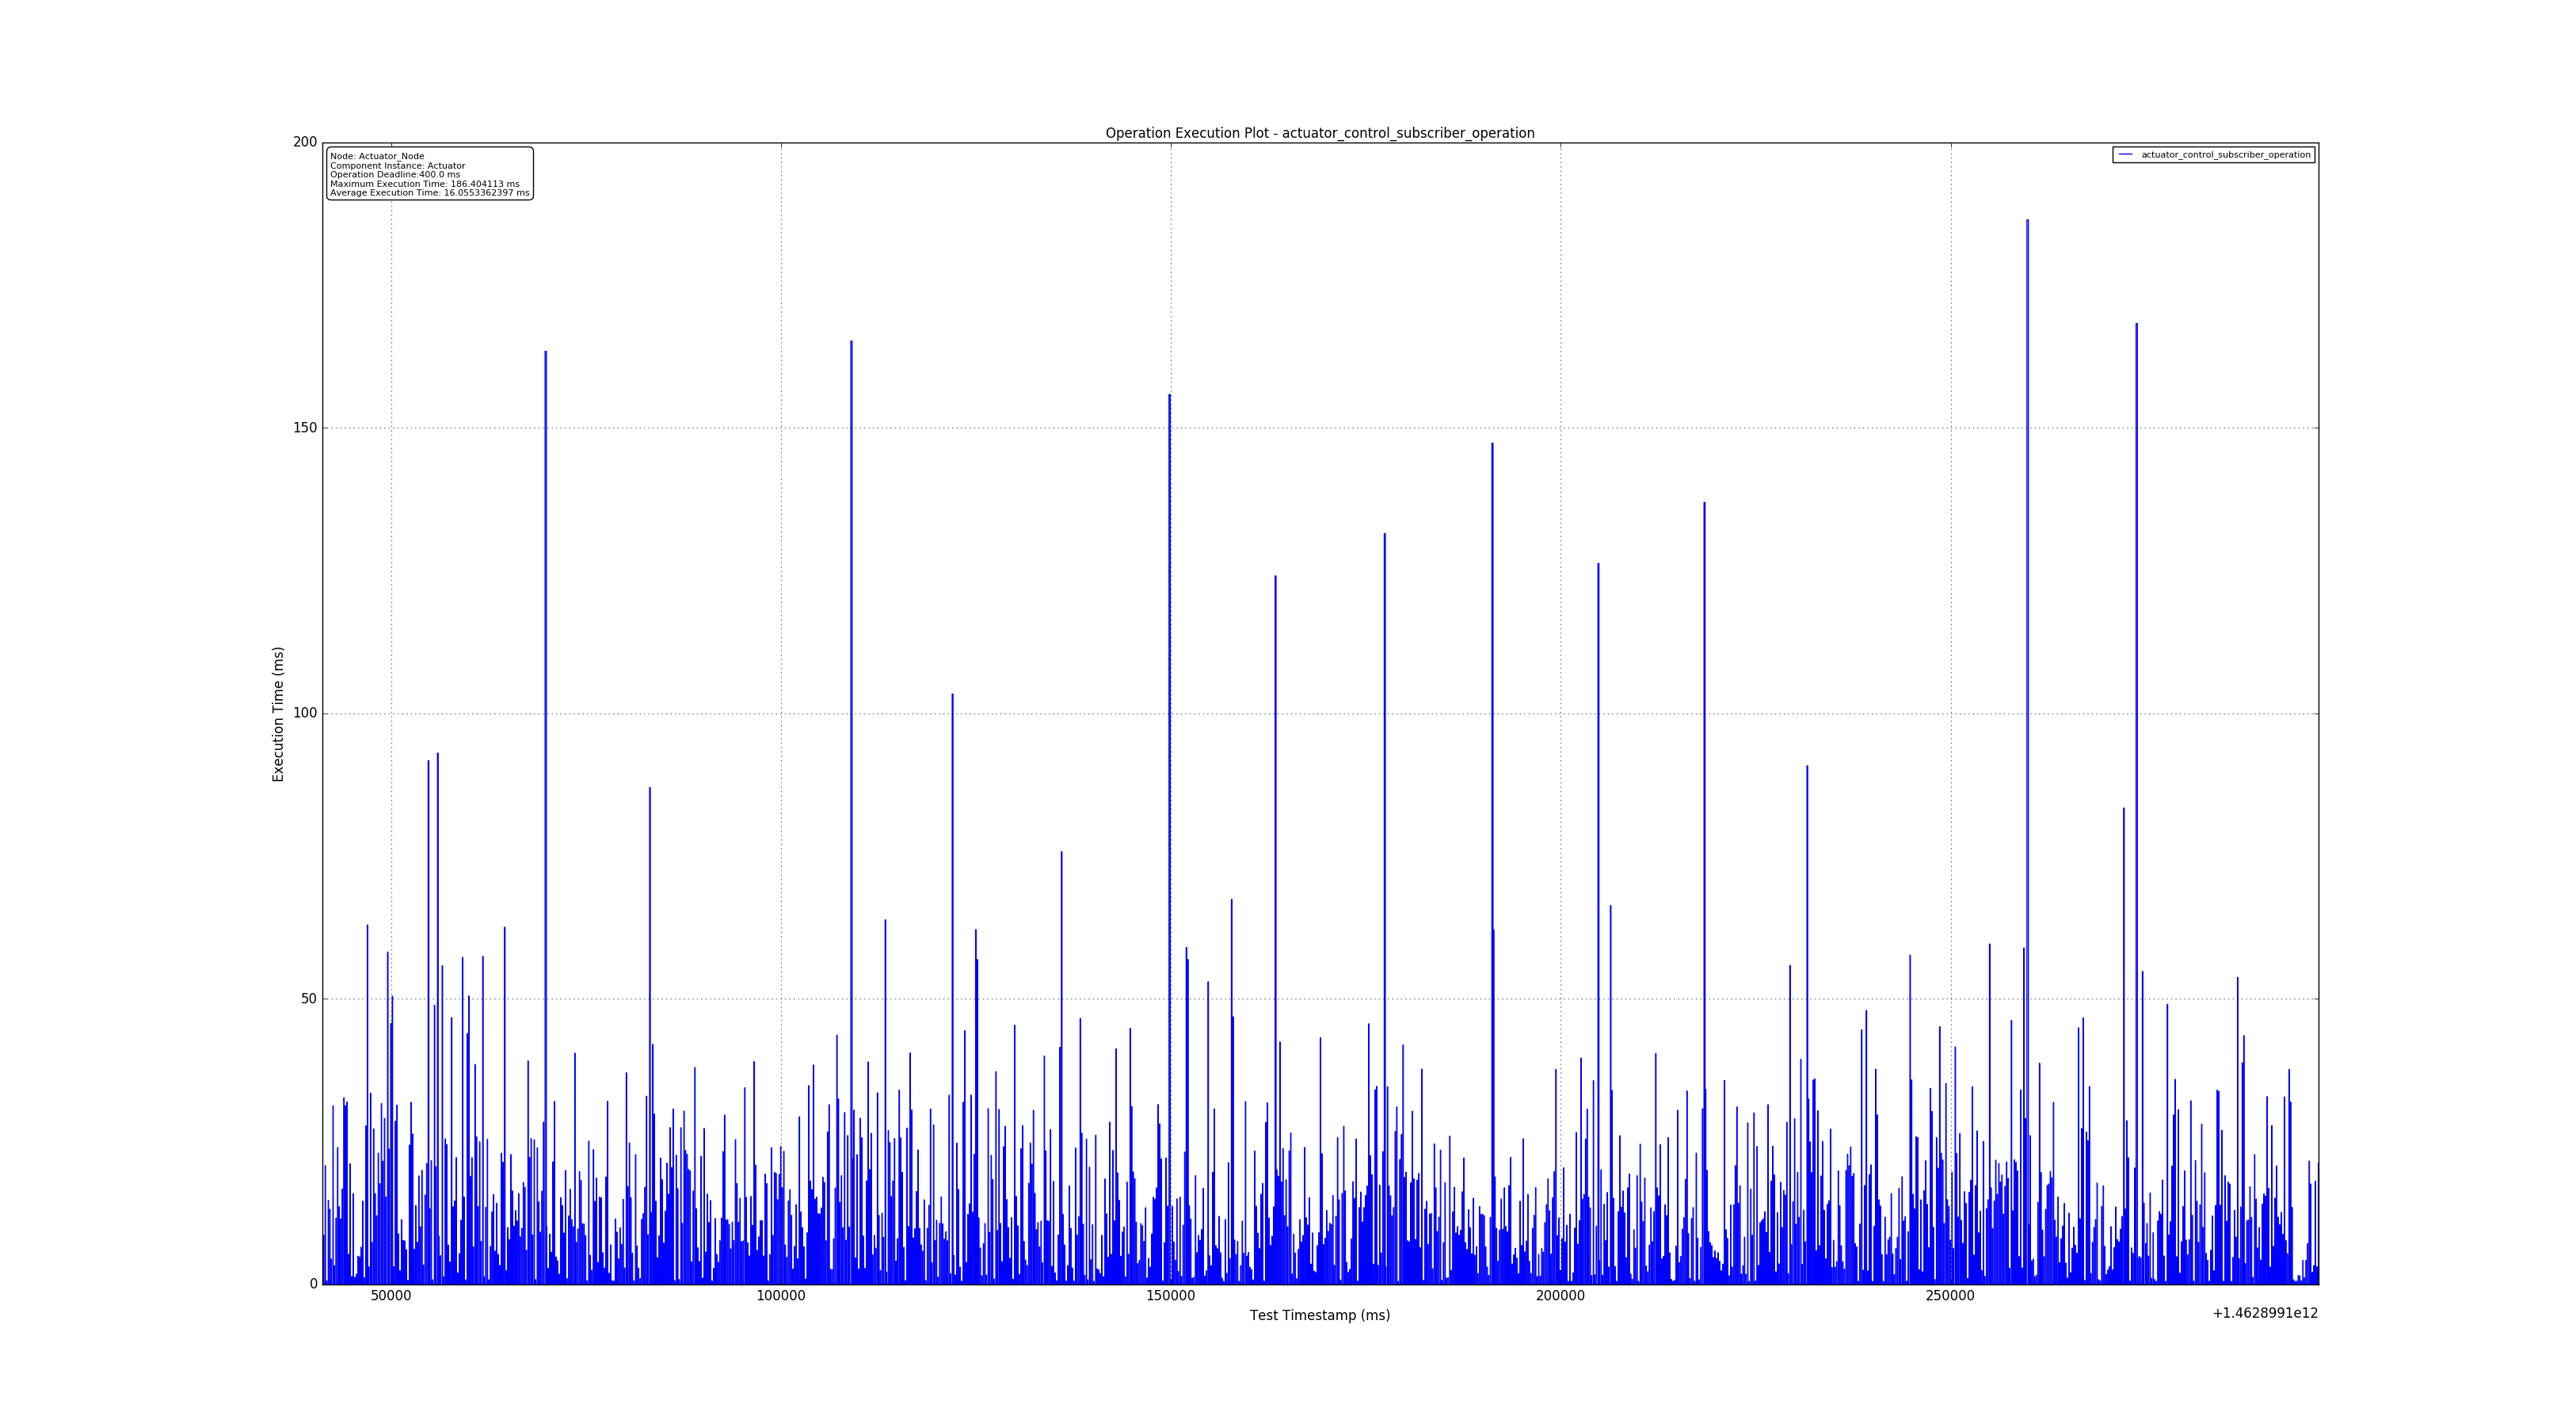
\includegraphics[width=\textwidth]{ksp_actuator}
	\caption{Stearwing Control - Actuator Component}
	\label{fig:ksp_actuator}
\end{figure} 
\FloatBarrier 


\subsubsection{Implementation and Results}

\begin{figure}[h]
	\centering
	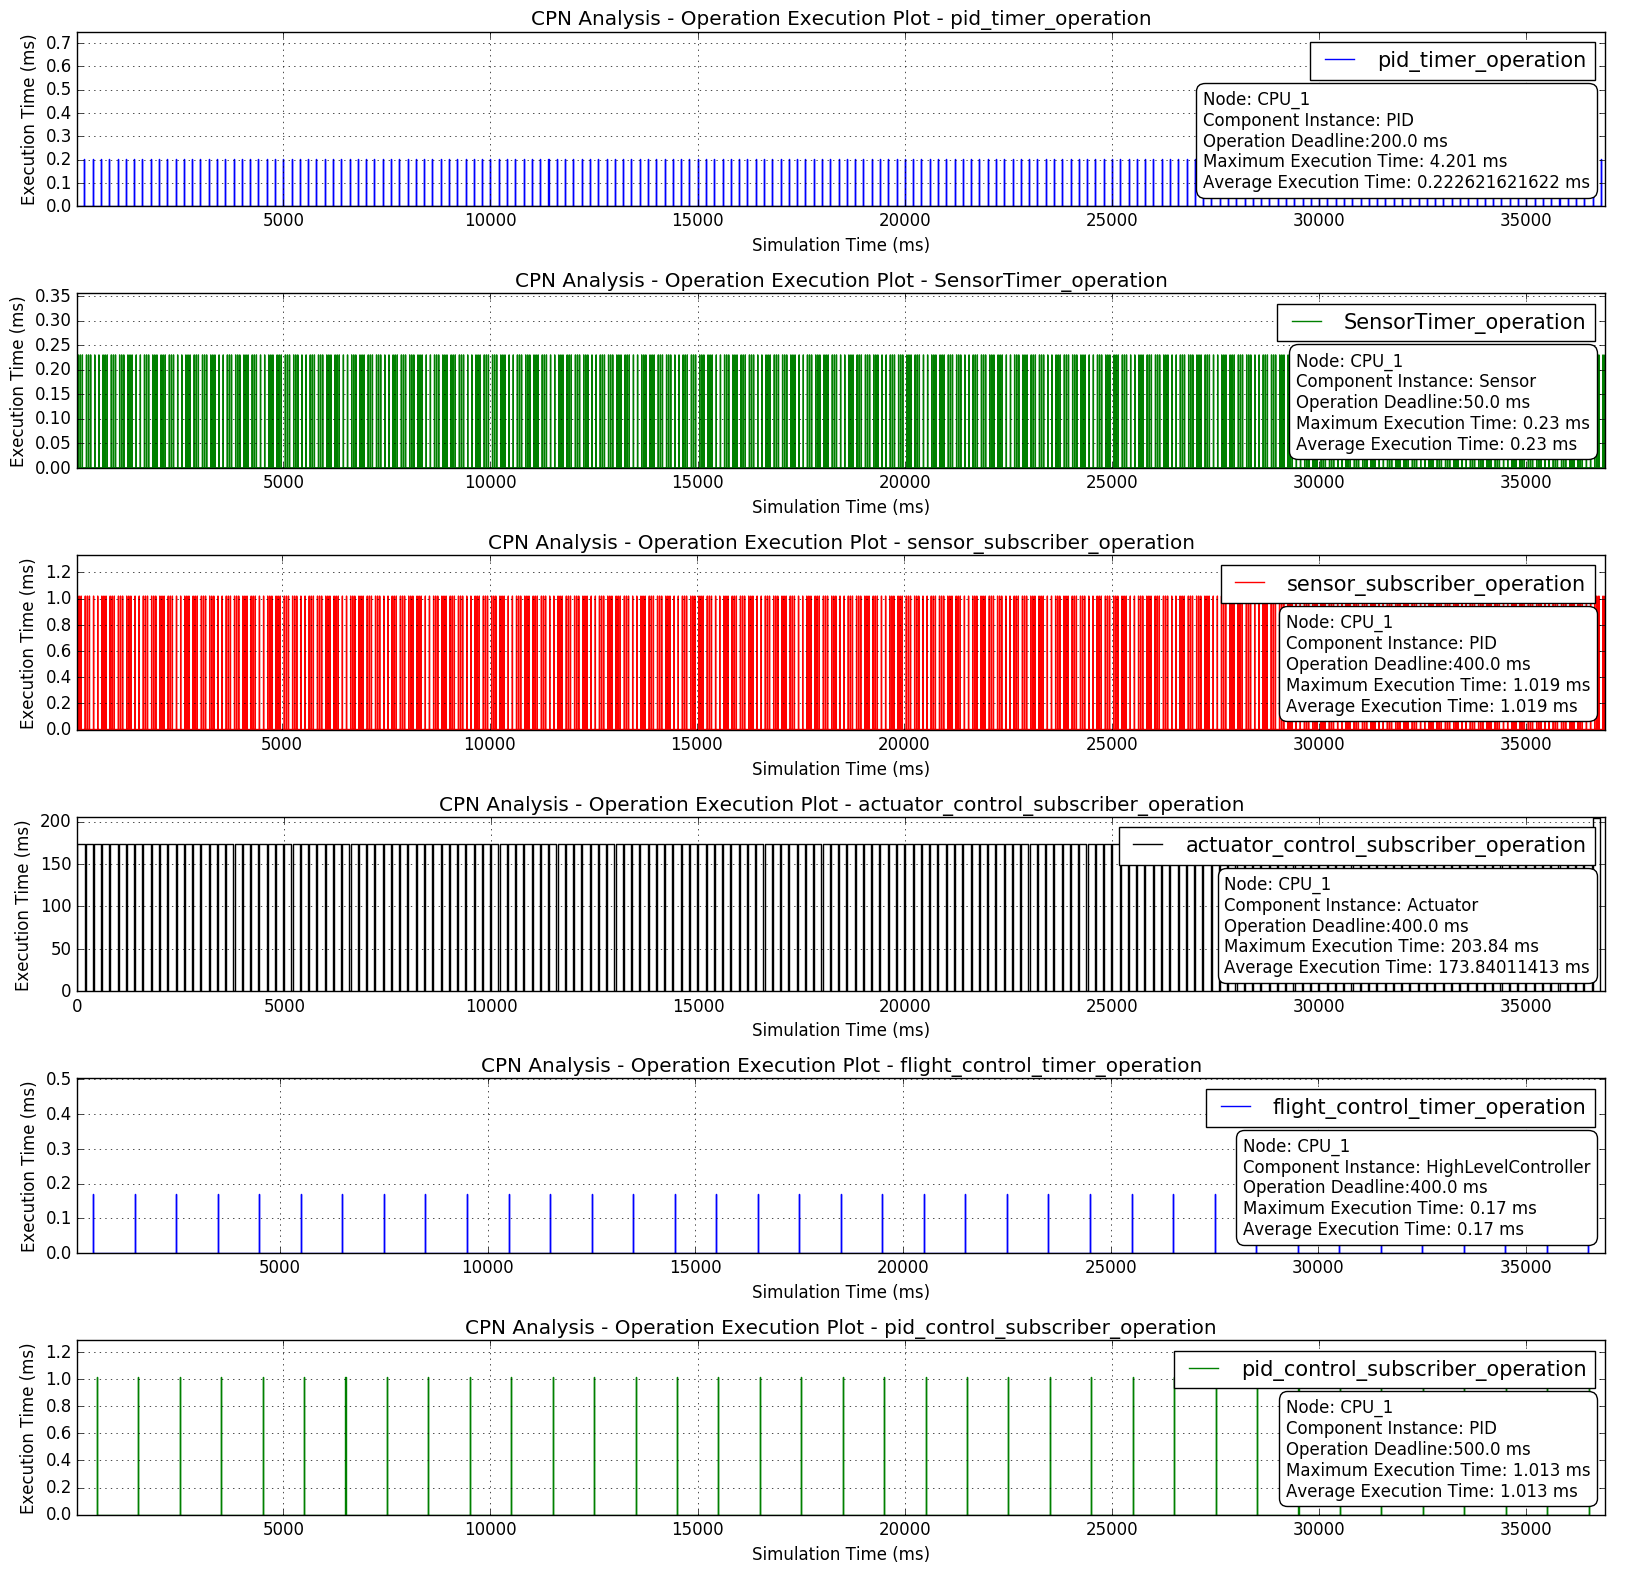
\includegraphics[width=\textwidth]{ksp_cpn}
	\caption{Stearwing Control - CPN Analysis Results}
	\label{fig:ksp_cpn}
\end{figure} 
\FloatBarrier 

\section{Analysis Limitations}

The business logic abstraction, as presented in Section \ref{sec:BL_Model}, is quite simple. This model represents abstractly how long the different blocks of code in an operation take, but does not fully model its behavior e.g. each non-blocking local code block is represented by a single WCET and no other properties. Since variables local to these functional code blocks are not modeled, this grammar also does not model conditional behavior. So, a high-level controller component that executes an event-driven state machine cannot be sufficiently modeled with the current model. Moreover, depending on the local state of such code blocks, different interaction patterns may be invoked e.g. if this high-level controller was responsible for performing periodic image processing to identify an object, the image processing (and all the associated image processing) would stop once the object was identified. Since this conditional interaction is not modeled in the CPN business logic grammar, the abstraction would assume that the image processing interactions always happen, instead of conditionally. Such abstractions can lead to gross over-estimation of the worst-case execution times of component operations. The primary reason for keeping the business logic grammar to this level of simplicity is to reduce the level of state space explosion i.e. modeling all local variables of an operation, and consequently the state changes for each of these variables would exponentially increase the size of the state space to be analyzed. Also, modeling the local variable state would also require (1) modeling the semantics of language with which the operation code was written, (2) evaluating all expressions using these local variables, and (3) calculating the result of all conditionals used in the business logic at all possible times. Such an analysis would be too refined, hard to implement and susceptible to semantic errors. 




\chapter{Summary and Future Work}
\label{chapter:conclusion}

% Summarize Contributions first
This thesis has presented an integrated timing analysis methodology for component-based distributed real-time embedded systems. The approach works by translating a design model of the target system i.e. a precise model of the software, hardware, and deployment into a Colored Petri net (CPN) and evaluating the system by performing state space analysis on the net. In the thesis, the DREMS component model is chosen as the target model for analysis. Aspects of the DREMS component e.g. the execution semantics of the component operation scheduler, the semantics of port interactions etc. are encoded as functions in Standard ML and integrated into the CPN model. User-defined properties of a DREMS component e.g. the component definition, the properties of component timers and ports, the connections between components etc. are parsed and translated into CPN tokens and injected into the generic model. Once injected, the complete CPN model is then analyzed using state space analysis queries. A state space is a directed graph, where the nodes represent states of existence of the system, and the edges between nodes represent transitions between the states of existence. State space analysis is the process of searching through the possible states of existence of the system to identify a state or a set of states where some system property is violated e.g. response time of some component operation has violated its timing specification. Not only is the CPN analysis model completely generated from the system design model, it is also capable of analyzing a variety of different system properties such as deadline violations, trigger-to-response times, deadlock freedom and CPU utilization. Scalability studies indicate that the model is capable of analyzing medium-to-large scale systems and experimental evaluation shows that the predicted execution time bounds for component operations are conservative but close approximations of the real execution.

All of the results presented in this thesis make an important assumption about the network -- the network resources available to each component is much larger than the requirements of the application i.e. there are no buffering delays on the network queues when components periodically produce data. The current analysis model, in this respect, is quite lacking. When a component publishes a message on a topic, the analysis immediately generates a reception message that waits to enqueue on the receiver's message queue. In reality, this interaction could be a lot more involved -- the published message is sent to the kernel network queue on the sender's side and removed from this queue following a data production \emph{profile} i.e. available bandwidth as a function of time. When dequeued, the packets take a finite worst-case transmission time before being noticed on the receiver's side. The buffering delays on the sender's side and the transmission time on the network are completely ignored by the timing analysis model. In order to improve on this design, we have attempted to integrate existing Network Calculus-based analysis methods \cite{ISIS_F6_CYPHY:14} into our CPN. Specifically, a place is added to model the \emph{Network Queue} and a \emph{Dequeue} transition fires when the network is ready to transport more packets from the sender. The dequeuing follows a strict network profile and ceases transmission when the data production rate is larger than the available bandwidth. 

Also, the business logic model i.e. the model of execution code in a component operation is quite simplistic. This model is able to represent local non-blocking code blocks, DREMS-style interaction patterns, and bounded loops of either. The model is however, unable to represent conditional statements that rely on local variables. This is a disadvantage as the resultant analysis is unable to accurately represent the execution behavior of the runtime code. Many if not most distributed real-time embedded scenarios in real-life exhibit conditional behavior that are driven by runtime state e.g. robotic applications that transition from one state of operation to another at runtime. The business logic of such operations cannot be fully represented by the current model and this has lead to gross overestimates in execution time behavior. Such over-estimation makes the analysis results useless as no operation scheduling may be calculated as feasible. Thus, the business logic model, and its integration into the analysis model both require improvement in order to support a wider range of execution scenarios. 


\chapter{Conclusions}

In this proposal, we have described the class of distributed real-time embedded software systems we are addressing. We have provided detailed descriptions and reviews of relevant related work, covering a wide range of analysis tool suites. We have also briefed about the DREMS infrastructure, the backbone of the proposed research and development. We have elaborated on the Colored Petri net-based timing analysis methodology, describing both the modeling aspects and analysis results. The subsequent sections describe some interesting  heuristics and modeling changes that greatly improved our analysis results, especially for distributed deployment scenarios. The remaining challenges within this scope include an experimental validation of the presented work and potential extensions to model and analyze Cyber-Physical systems. 
\begin{appendices}

\chapter{Publications}

\label{ch:publications}

The full text in each of the following papers was reviewed by at least 3 reviewers.

\section{Workshop Papers}
\nobibliography*{}
\begin{itemize}
	\item \bibentry{kumar2014colored}
	\item \bibentry{SEUS}
	\item \bibentry{SEUS2016}	
\end{itemize}

\section{Conference Papers}
\begin{itemize}
	
	\item P. Kumar, W. Emfinger, A. Kulkarni, G. Karsai, D. Watkins, B. Gasser, C. Ridgewell, and A. Anilkumar. ROSMOD: A Toolsuite for Modeling, Generating, Deploying, and Managing Distributed Real-time Component-based Software using ROS. In \textit{Proceedings of the IEEE Rapid System Prototyping}, RSP 2015, Amsterdam, Netherlands, 2015. IEEE	
	
	\item P. Kumar, W. Emfinger, and G. Karsai. A Testbed to Simulate and Analyze Resilient Cyber-Physical Systems. In \textit{Proceedings of the IEEE Rapid System Prototyping}, RSP 2015, Amsterdam, Netherlands, 2015. IEEE	
	
	\item W. Emfinger, P. Kumar, A. Dubey, W. Otte, A. Gokhale, G. Karsai. DREMS: A Toolchain for the Rapid Application Development, Integration, and Deployment of Managed Distributed Real-time Embedded Systems. In \textit{Proceedings of the IEEE Real-Time Systems Symposium}, RTSS@Work 2013, Vancouver, Canada, 2013. IEEE
	
	\item Balasubramanian, D., W. Emfinger, P. S. Kumar, W. Otte, A. Dubey, and G. Karsai. An application development and deployment platform for satellite clusters.  In \textit { Proceedings of the Workshop on Spacecraft Flight Software}, 2013
	
	\item Balasubramanian, D., A. Dubey, W. R. Otte, W. Emfinger, P. Kumar, and G. Karsai. A Rapid Testing Framework for a Mobile Cloud Infrastructure.  In \textit{Proceedings of the IEEE International Symposium on Rapid System Prototyping}, RSP, 2014. IEEE
	
\end{itemize}

\section{Journal Papers}
\begin{itemize}
	\item \bibentry{balasubramanian2015drems}
	
	\item Levendovszky, T., A. Dubey, W. R. Otte, D. Balasubramanian, A. Coglio, S. Nyako, W. Emfinger, P. Kumar, A. Gokhale, and G. Karsai. DREMS: A Model-Driven Distributed Secure Information Architecture Platform for Managed Embedded Systems. In \textit{IEEE Software}, vol. 99: IEEE Computer Society, 2014. IEEE	
\end{itemize}

\subsection{Awaiting Reviews}
\begin{itemize}
	\item P. Kumar, W. Emfinger, G. Karsai, D. Watkins, B. Gasser, and A. Anilkumar. ROSMOD: A Toolsuite for Modeling, Generating, Deploying, and Managing Distributed Real-time Component-based Software using ROS. In special issue of \textit{Journal of Electronics} on Rapid System Design with Dedicated Architectures and Specific Software Tools, 2016.
\end{itemize}

\end{appendices}



\bibliographystyle{abbrv}
\begin{spacing}{1}
  \bibliography{00-Dissertation}
\end{spacing}
	
\end{document}
